% Author: Brandon Patterson
% Description: Paper about acoustically perturbed liquid-gas interfaces
% 
% 
% Use the article class.
\documentclass{article}
% 
% Title of the paper
\title{Acoustically accelerated liquid-gas interfaces}
% 
% Author name
\author{Brandon Patterson}
% 
% Year of completion
\year=\the\year
% 
%% Load packages
\usepackage{fullpage}
\usepackage{hyperref}
\usepackage{graphicx}
\usepackage{natbib}
\usepackage{pdflscape}
\usepackage{mathrsfs}
\usepackage{rotating}
\usepackage[usenames,dvipsnames]{xcolor}
\usepackage{tikz}
\usepackage{pgfgantt}
\usepackage{typearea}
\usepackage{abstract}
\usepackage{verbatim}
\usepackage{tabularx}
\usepackage{caption}
\usepackage{subcaption}
\usepackage{embedfile}
\usepackage{import}
\usepackage{amsmath}
\usepackage[nolist,nohyperlinks]{acronym}
\usepackage{soul}
% 
% Create a snapshot of dependencies and place in .dep file
\RequirePackage{snapshot}
% 
% My commands
\newcommand{\bs}[1]{\boldsymbol{#1}}
\newcommand{\del}[0]{\nabla}
\newcommand{\orderof}[1]{\ensuremath{\mathcal{O}\left(#1\right)}}
\newcommand{\abs}[1]{\ensuremath{\left|#1\right|}}
\newcommand{\norm}[1]{\ensuremath{\left\Vert#1\right\Vert}}
\newcommand{\plus}{\raisebox{.2\height}{\scalebox{.8}{+}}}
%
% 
% Embed files
\embedfile{./content/embed_files.tex}
\embedfile{./content/abstract.tex}
\embedfile{./content/intro.tex}
\embedfile{./content/methods.tex}
\embedfile{./content/analysis.tex}
\embedfile{./content/results.tex}
\embedfile{./content/conclusions.tex}
\embedfile{./content/future.tex}
%                                                               
%
%%% Local Variables:
%%% mode: latex
%%% TeX-master: "main"
%%% End:

\embedfile{./main.tex}
% 
% 
%% DOCUMENT AREA
\begin{document}
%% Definition of any abbreviations used.
\begin{acronym}%
   \acro{CEUS}{Contrast-Enhanced Ultrasound}
 \acro{CFD}{Computational Fluid Dynamics}
 \acro{DG}{Discontinuous Galerkin}
 \acro{DUS}{Diagnostic Ultrasound}
 \acro{HIFU}{High Intensity Focused Ultrasound}
 \acro{IC}{Inertial Cavitation} 
 \acro{LH}{Lung hemorrhage}
 \acro{MC}{Monte Carlo}
 \acro{PD}{Pulse Duration}
 \acro{PDF}{Probability Distribution Function}
 \acro{PFP}{Perfluoropropane}
 \acro{PRF}{Pulse Repetition Frequency}
 \acro{PRPA}{Peak Rarefaction Pressure Amplitude}
 \acro{RMI}{Richtmyer-Meshkov Instability}
 \acro{TL}{Transmission Loss}
 \acro{US}{Ultrasound}


%%% Local Variables:
%%% mode: latex
%%% TeX-master: "../main"
%%% End:
%
\end{acronym}%
\maketitle
\begin{center}
  \begin{minipage}{0.8\textwidth}
    \subsection*{Abstract}
    \ac{DUS} of the lung has been shown to cause hemorrhage in a
    variety of mammals, though the underlying damage mechanism is yet
    to be determined. Motivated by this problem we model an alveolar
    tissue-air interface as a perturbed water-air interface and
    simulate its interaction with trapezoidal acoustic waves to
    investigate the underlying physics. We find that baroclinic
    vorticity is generated along the interface as a result of
    misalignment between acoustic pressure gradients and the density
    gradients across the interface. This vorticity remains continues
    to deform the interface long after all of the acoustic waves have
    passed. We postulate that this nonlinear effect is important
    because of the sharp density gradient that occurs at the water-air
    interface.

    Unlike shocks, whose interactions with fluid-fluid interfaces is
    well studied and nearly instantaneous, the acoustic waves
    considered here interact with the interface over variable, finite
    amounts of time. The effect of this interaction time is shown to
    have a significant impact on the growth of the interface
    perturbation for acoustic waves of similar amplitude and shape. We
    show that this is a result of changes in vorticity deposition that
    occur due to interface deformation that occurs during the
    interaction with the
    wave.

    Finally, We additionally perform analysis to predict the location
    of vorticity generation and growth of the interface, which we
    compare to the observed computational results.
  \end{minipage}
\end{center}
%%% Local Variables:
%%% mode: latex
%%% TeX-master: "../main"
%%% End:

\acresetall
\section{Introduction}%
\label{sec:introduction}%
%
\ac{DUS} is one of the safest forms of medical imaging and has become
ubiquitous in clinical practice, however it has been demonstrated to
trigger lung hemorrhage in a variety of animals. While the problem
does not appear to be one of significant medical concern under common
clinical conditions, the underlying cause is not well understood and
more information is needed so that future developments in ultrasound
remain safe. The purpose of this work is to investigate the underlying
physics of acoustically accelerated liquid-gas interfaces such as
those in the lungs. 

%
Over the last few decades \ac{DUS}-induced \ac{LH} has been
studied extensively and is the only known bioeffect of non-contrast,
pulsed \ac{US} known to occur in mammals. It has been demonstrated in
a variety of animal models including mice, rats, rabbits, pigs, and
monkeys \citep{Child1990,OBrien2006a,Tarantal1994a}. Presently the
physical damage mechanisms underlying the hemorrhage are not well
understood.

\ac{DUS}-induced \ac{LH} does not appear to be caused by traditionally
expected \ac{US} bioeffects mechanisms. Typically, \ac{US} bioeffects
mechanisms are classified as thermal or non-thermal with the bulk of
non-thermal bioeffects being a result of acoustic cavitation. Thermal
mechanisms have shown to be an unlikely cause of lung hemorrhage, as
\cite{Zachary2006} found that \ac{DUS}-induced lung lesions do not
appear similar to those induced by heat. There has also been
significant research suggesting that \ac{IC} is also an unlikely
damage mechanism for \ac{DUS}-induced \ac{LH} as \cite{OBrien2000}
observed that the severity of \ac{DUS}-induced \ac{LH} in mice
increased under raised hydrostatic pressure, and \cite{Raeman1996}
found that the hemorrhage is unaffected by the introduction of \ac{US}
contrast agents. One study reports detecting cavitation during
\ac{DUS}-lung interaction in rats \cite{Holland1996}. \cite{Tjan2007}
proposed that focused ultrasound may lead to the ejected of droplets
capable of puncturing the air-filled sacs within the lung, and
performed numerical simulations of as an inviscid, free surface
subjected to a Gaussian velocity potential to show that the proposed
droplet ejection may occur under certain circumstances. Similarly,
\cite{Simon2012} observed \ac{HIFU} induced atomization of tissue at
air interfaces. Despite these efforts, the precise damage mechanism
underlying \ac{DUS}-induced \ac{LH} is still unknown. And while
\ac{DUS} of the lung has not been observed to cause medical problems
in humans under typical clinical conditions, it is an important
problem to understand if we hope to further develop and improve
\ac{DUS} by expanding the physical regimes in which it operates.

Within the fluids community, there has been extensive research into
the fundamental physics describing interactions between mechanical
waves and fluid interfaces. However, much of this research is
motivated by applications in fusion energy and astrophysics and
accordingly has sought to investigate regimes outside of those of
acoustic interests. One topic of considerable past study is the
\ac{RMI}, in which a perturbed fluid-fluid interface is accelerated by
a shock, causing the interface perturbation to grow
\citep{Brouillette2002,Drake2006}. This growth is driven by a sheet of
baroclinic vorticity deposited along the interface as a result of
misalignment between the pressure gradient across the shock and the
density gradient across the perturbed interface. This physical
mechanism by which these misaligned gradients create a torque on fluid
particles and generate vorticity can be thought of in terms of a
hydrostatic balance upon a particle. Pressure gradients result in
acceleration of the flow. This acceleration is inversely proportional
to density. When these two gradients are misaligned, the result is a
shear stress on the fluid and vorticity is generated. An excellent
graphical explanation of this can be found in \cite{Heifetz2015}.
Analytically, baroclinic vorticity generation can be shown by taking
the curl of the conservation of momentum equation for a compressible
fluid. However we note that it is a nonlinear effect and cannot be
explained by traditional linear acoustics.
% \begin{figure}
%   \centering
%   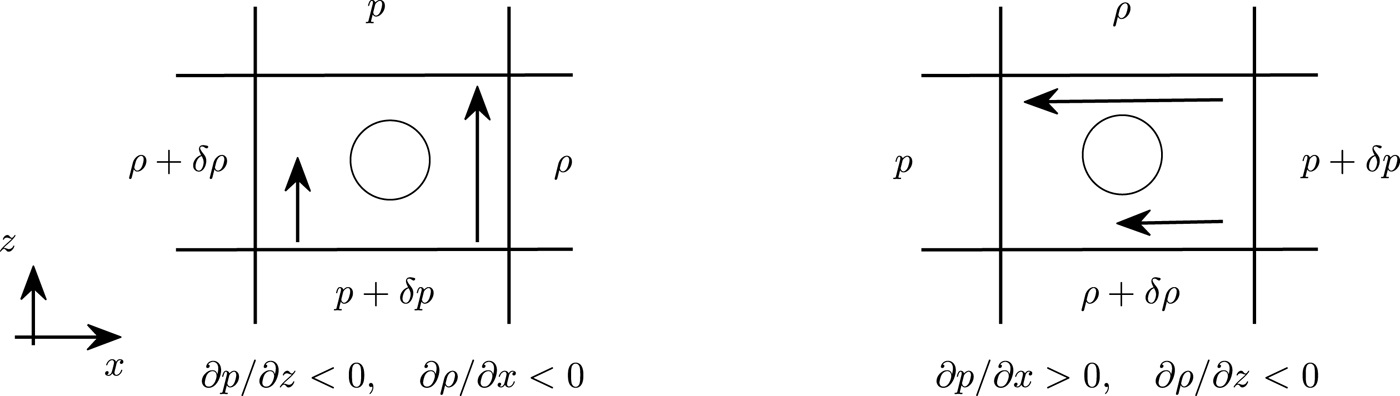
\includegraphics[width=0.9\textwidth]{./figs/lung_figs/baroclinic_schematic} \hfill
%   \caption[A schematic of baroclinic torque]{From
%     \cite{Heifetz2015}. A hydrostatic force balance upon a particle
%     subject to perpendicular pressure and density gradients
%     illustrates baroclinic torque on a fluid particle.}
%   \label{fig:usbe_lung_baroclinic_schematic}
% \end{figure}

The physics of the \ac{RMI} are fairly well understood. For the classical \ac{RMI}
setup a planar shock impinges normally upon the peaks and troughs of a
sinusoidal interface. As the degree of misalignment varies along the
interface, the interface is accelerated non-uniformly. The direction
of the vorticity changes where the slope of the interface
changes. This counter rotation on either side of interface peaks and
troughs entrains nearby fluid causing interface peaks to accelerate in
one direction and troughs to accelerate in the opposite
direction. This results in a ``bubble'' of light fluid penetrating the
heavy fluid, and a ``spike'' of heavy fluid penetrating the light
fluid. How exactly this occurs varies slightly depending on the
relative densities of the two fluids. For the case of a wave moving
from a light fluid into a heavy one, the peaks and troughs of the
interface are initially accelerated to move away from one another, and
the interface perturbation amplitude undergoes growth exclusively. For
the case of a wave moving from a heavy fluid to a lighter fluid, the
peaks and troughs of the interface are accelerated such that they
initially move closer to one another decreasing the perturbation
amplitude. They then pass one another, inverting the phase of the
interface perturbation, and then continue moving in opposite
directions, growing the perturbation amplitude. This process is
illustrated in Figure \ref{fig:rmi_schematic}, which has been adapted
from \cite{Brouillette2002}.
\begin{figure}
  \centering
  \def\svgwidth{0.9\textwidth}
  \import{./figs/lung_figs/}{brouillette_fig3_mod.pdf_tex} \hfill%
  \caption[A schematic view of the \ac{RMI} instability for a
  heavy-light interface]{Adapted from \cite{Brouillette2002}. The
    \ac{RMI} for a heavy-light interface is illustrated. The initial
    condition (left), circulation post wave-interface interaction
    (center), and perturbation growth (right) are shown.}
  \label{fig:rmi_schematic}
\end{figure}

Previous studies of the \ac{RMI} have utilized theory, computation, and
experiments to describe the behavior of the interface after the wave
has passed. \cite{Richtmyer1960} performed the linear stability
perturbation analysis developed by \cite{Taylor1950} for the case of
an impulsive acceleration to create a model for the initial growth of
the interface perturbation. \cite{Meshkov1969} experimentally
confirmed Richtmyer's qualitative predictions, hence the name of the
instability. \cite{Meyer1972} performed numerical simulations of the
\ac{RMI} and found good agreement with Richtmyer for the case of a
shock impinging upon a light-heavy interface. \cite{Fraley1986} used
Laplace transforms in order to find the first analytical solution for
the asymptotic growth rate for a shocked interface between perfect
gases. To describe the late time, nonlinear growth of the
perturbation, \cite{Zhang1997} used single mode perturbation, keeping
many high order terms, to describe the velocity of the bubble and
spike regions of the fluid. \cite{Sadot1998} combined the linear,
impulsive solution with potential flow models of the asymptotic
behavior of the bubble and spike to develop a model for the
perturbation growth that is in good agreement with shock tube
experiments for shocks with Mach numbers Ma=1.3, 3.5. Vortex theory
has also been used to describe the behavior of the
interface. \cite{Jacobs1996} horizontally oscillated a container with
two vertically stratified liquids to obtain standing waves and then
bounced the container off of a coil spring to study the incompressible
\ac{RMI}. The late time evolution of is interface is modeled using a
row of line vorticies to obtain qualitatively similar results to those
experimentally observed, however the late-time growth rate is
underestimated. \cite{Samtaney1994} used shock polar analysis to find
the circulation deposited by a shock on planar and non-planar
interfaces. Their results are validated using and Euler code and found
to be within 10\% of the computed value for $1.0\,<\,$Ma$\,\leq\,1.32$
for all $\rho_2/\rho_1\,>\,1$, and
$5.8\,\leq\,\rho_2/\rho_1\,\leq\,32.6$ for all Ma. This work aims to
add to the current body of work on this topic by investigating
interfaces accelerated by pressure waves within the acoustic regime.

% Accordingly we propose a possible damage mechanism of
% \ac{DUS}-induced \ac{LH}. We hypothesize that misalignment between
% the pressure gradients in the \ac{DUS} pulses and density gradients
% within the lungs create torque at the alveolar walls, which deform
% and ultimately hemorrhage as a result.

The detailed nonlinear interactions between acoustic waves and
perturbed liquid-gas interfaces do not appear to have been previously
studied in this manner or context. This work is separate from previous
research into the \ac{RMI} as a result of the acoustic regime
considered here. Unlike shock waves, which occur over a few molecular
mean free paths and interact nearly instantaneously, acoustic waves
have a finite spacial wavelength and can occupy a much larger portion
of space. Consequently, their interaction with interfaces occurs over
a longer period of time depending on the waveform and the geometric
and material properties of the media. This duration can also be
thought of in terms of the relative sizes of the physical features of
the interface and the wavelengths of each feature of the acoustic wave
of interest. Simple \ac{RMI} analysis assumes an impulsive
acceleration, and does not apply to this work because the interface
deforms throughout its interaction with the wave.

Additionally, we argue that the basic problem setup of the \ac{RMI}, a
mechanical wave impinging upon a material interface, has many
physical similarities to the motivating problem of \ac{DUS} of the
lungs. While the pressure gradient due to the \ac{US} pulse is not as
sharp as it would be across the shock, there is a strong density
discontinuity across the tissue-air interfaces of the
lungs. Accordingly, we study problem geometries and acoustic waves
within the regimes of \ac{DUS} of the lung.

In the remainder of this work we will first present a model problem
and a set of numerical experiments designed to investigate the
fundamental physics underlying interactions between acoustic waves and
perturbed interfaces between fluids. We will present results that
specifically explore the dependence of the interface dynamics on
acoustically relevant properties including the amplitude and
wavelength of the acoustic wave. We pay particular attention to the
finite duration of the wave-interface interaction, and the interface
deformation that occurs during this period. We perform analysis to
explain the vorticity deposition and late time behavior of the
interface after all acoustic waves have passed. The results will be
discussed to address the following questions:
\begin{enumerate} \label{itm:usbe_lung_questions}
\item Are acoustic waves capable of generating sufficient baroclinic
  vorticity at perturbed liquid-gas interfaces for substantial
  deformations?
\item What is the impact of the acoustic wave properties, such as
  amplitude and wave duration, on the vorticity and interface
  dynamics?
\end{enumerate}
We will then discuss on the significance of these results as
they regard to the motivating problem of \ac{DUS}-induced lung
hemorrhage. We will finally end by summarizing the main conclusions
drawn from this work and suggest the next steps to be taken.



% \hl{ (MOVE ALL THIS TO LATER)
% We consider a compressible multi-fluid system and
% solve the Euler equations of inviscid fluid motion to study the
% dynamics of fluid-fluid interfaces exposed to acoustic waves relevant
% to \ac{DUS}. We observe that acoustically-generated vorticity at
% perturbed water-air interfaces drives the interface to deform. We
% hypothesize that a similar mechanism may be responsible for deforming
% and ultimately rupturing the fragile tissue barriers around alveoli,
% tiny air sacs within the lungs, leading to \ac{DUS} induced \ac{LH}.}




%%% Local Variables:
%%% mode: latex
%%% TeX-master: "../main"
%%% End:

\section{Methods} \label{sec:methods}%
In this section, we describe the set of numerical experiments designed
to investigate the fundamental fluid dynamics associated with
acoustically-accelerated, perturbed liquid-gas interfaces.

\subsection{Problem set-up}
\label{subsec:setup}
\begin{figure}
  \centering
  % 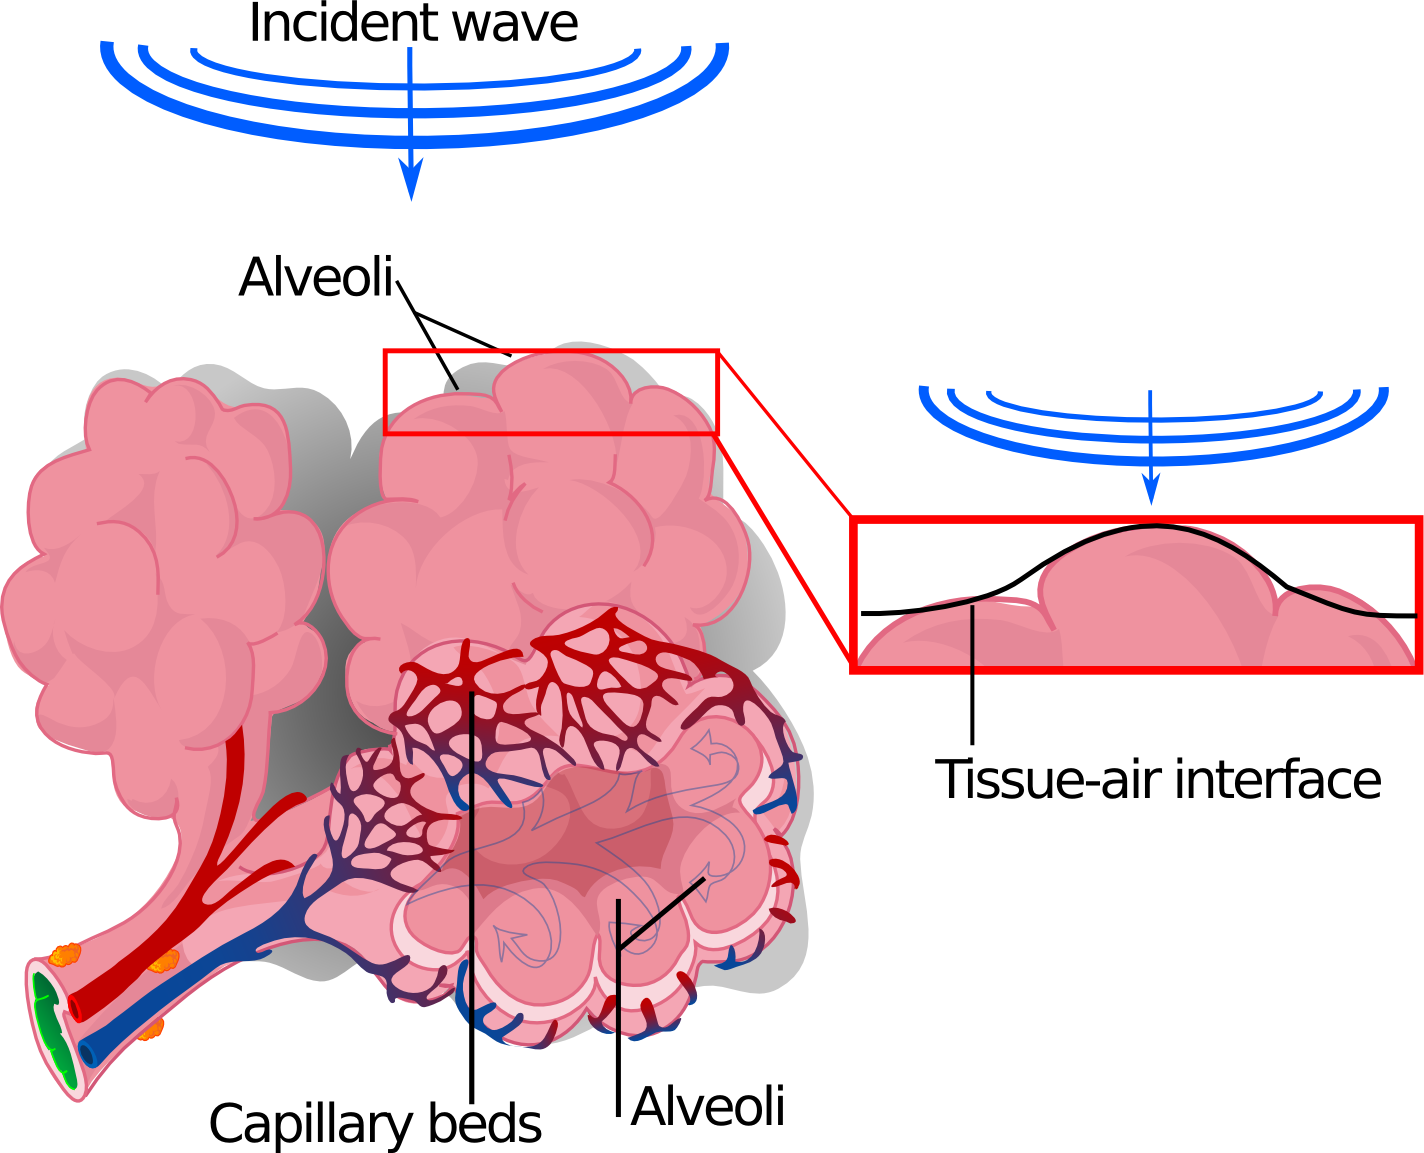
\includegraphics[width=0.48\textwidth]{./figs/lung_figs/Alveolus_US_zoom_diagram.pdf_tex} \hfill
  % \def\svgwidth{0.48\textwidth}
  % \import{./figs/lung_figs/}{usbe_lung_schematic2.pdf_tex} \hfill%
  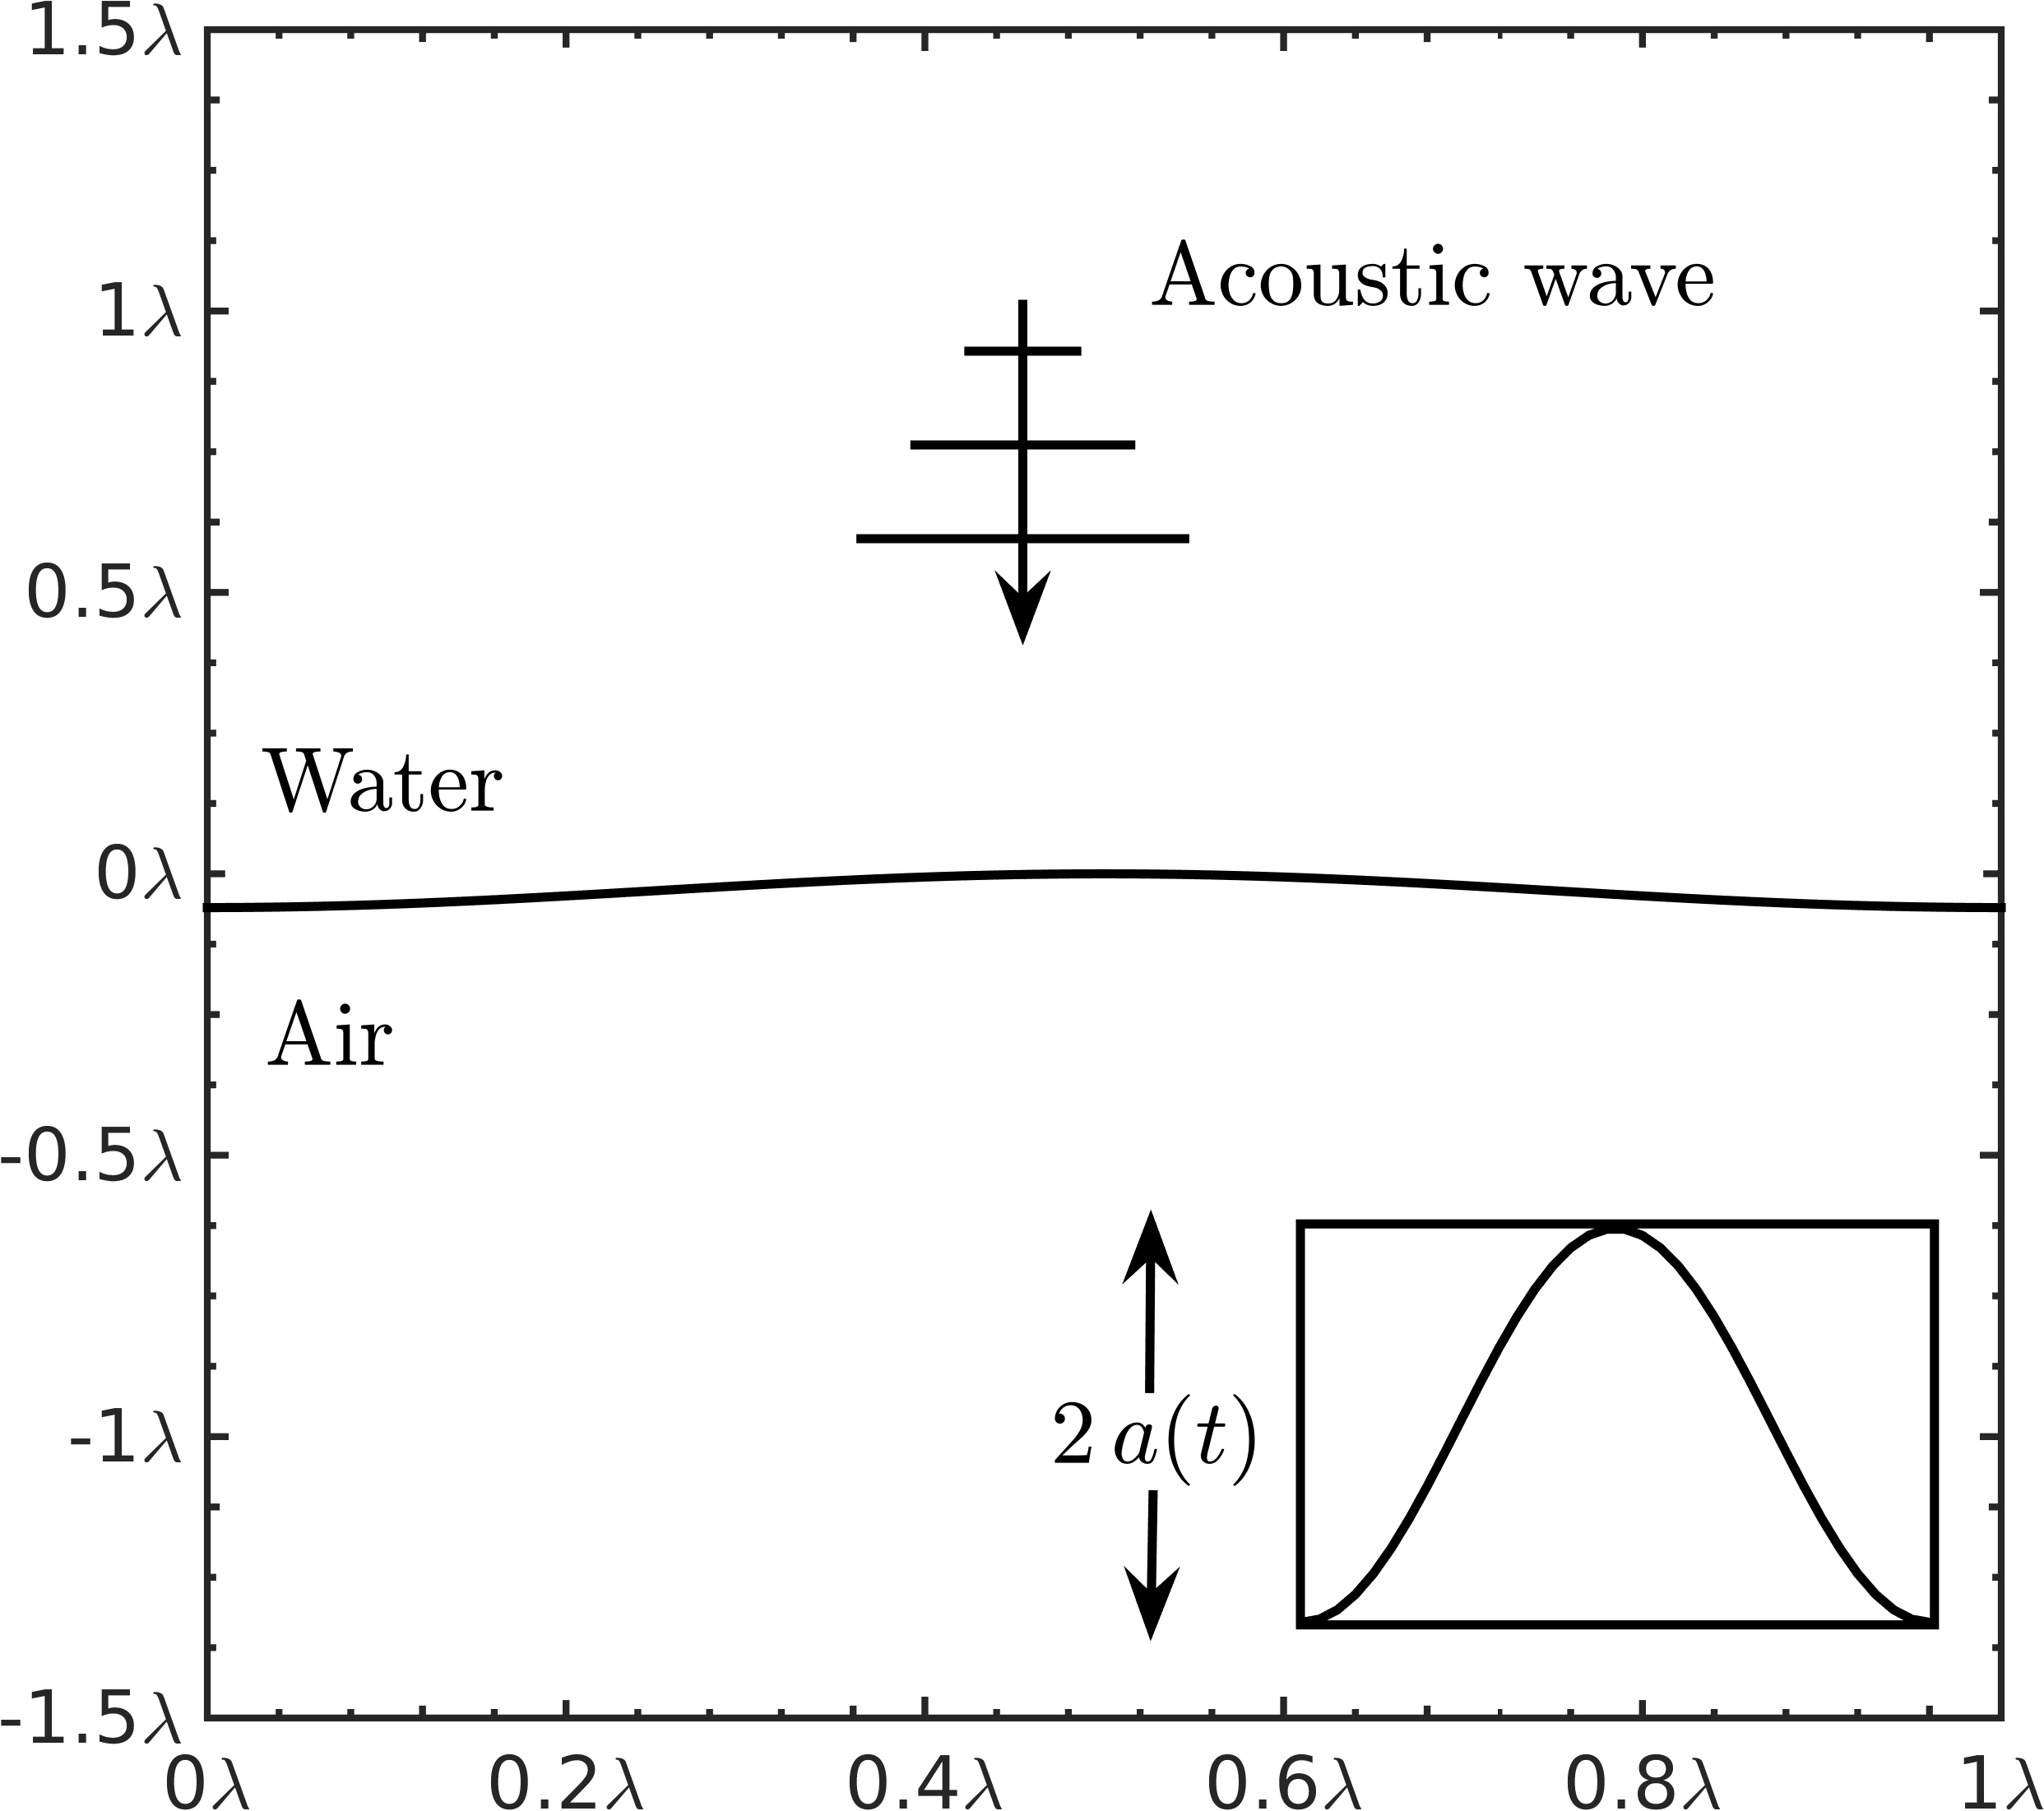
\includegraphics[width=0.48\textwidth]{./figs/lung_figs/usbe_model_schematic2} \hfill
  \caption[A schematic view of the model problem]{A schematic view of the initial and boundary conditions of the
    numerical experiments performed. An acoustic wave travels from water toward a sinusoidally perturbed water-air interface.}
  \label{fig:problem_schematic}
\end{figure}
% 
We consider a 2D, compressible inviscid fluid system in the $xy$-plane
with an acoustic wave impinging from water (top) downward toward air
(bottom). The water-air interface is initially located at the origin
and has a sinusoidal shape with wavelength $\lambda$ and amplitude
$0.03\lambda$ as seen in Figure \ref{fig:problem_schematic}. The width
of the rectangular computational domain is $1\lambda$ such that it is
traversed by a single period of the interface. This interface geometry
is consistent previous studies of the \ac{RMI}
\citep{Brouillette2002}.

As the primary focus of this study is on the fundamental physics of
acoustically-accelerated perturbed liquid-gas interfaces a very simple
acoustic waveform that can be studied analytically is optimal for our
purposes. As such, we choose initially symmetric trapezoidal waveforms
for the numerical experiments as illustrated in Figure
\ref{fig:p0}. The wave is composed of three stages, described here in
the order that they encounter the interface. First, compression
occurs, the pressure increases linearly from atmospheric to a maximum
of $p_a=1, 5$, or $10$ MPa gauge pressure. Second, the elevated
pressure $p_a$ is held constant over a fixed period. Note
that the subscript $_a$ will be used from here on to denote properties
of the acoustic wave. Third, an expansion occurs and pressure
decreases linearly back to atmospheric pressure. The pressure rise and
fall initially occur over equal distances $5\lambda$, such that they
have constant, equal spatial slopes $\pm p_{a}/5\lambda$. Unless
otherwise stated, the period of constant pressure has length
$35\lambda$ and thus the total length $L$ of the incoming acoustic wave is
$45\lambda$.
% 
\begin{figure}% 
  \centering%
  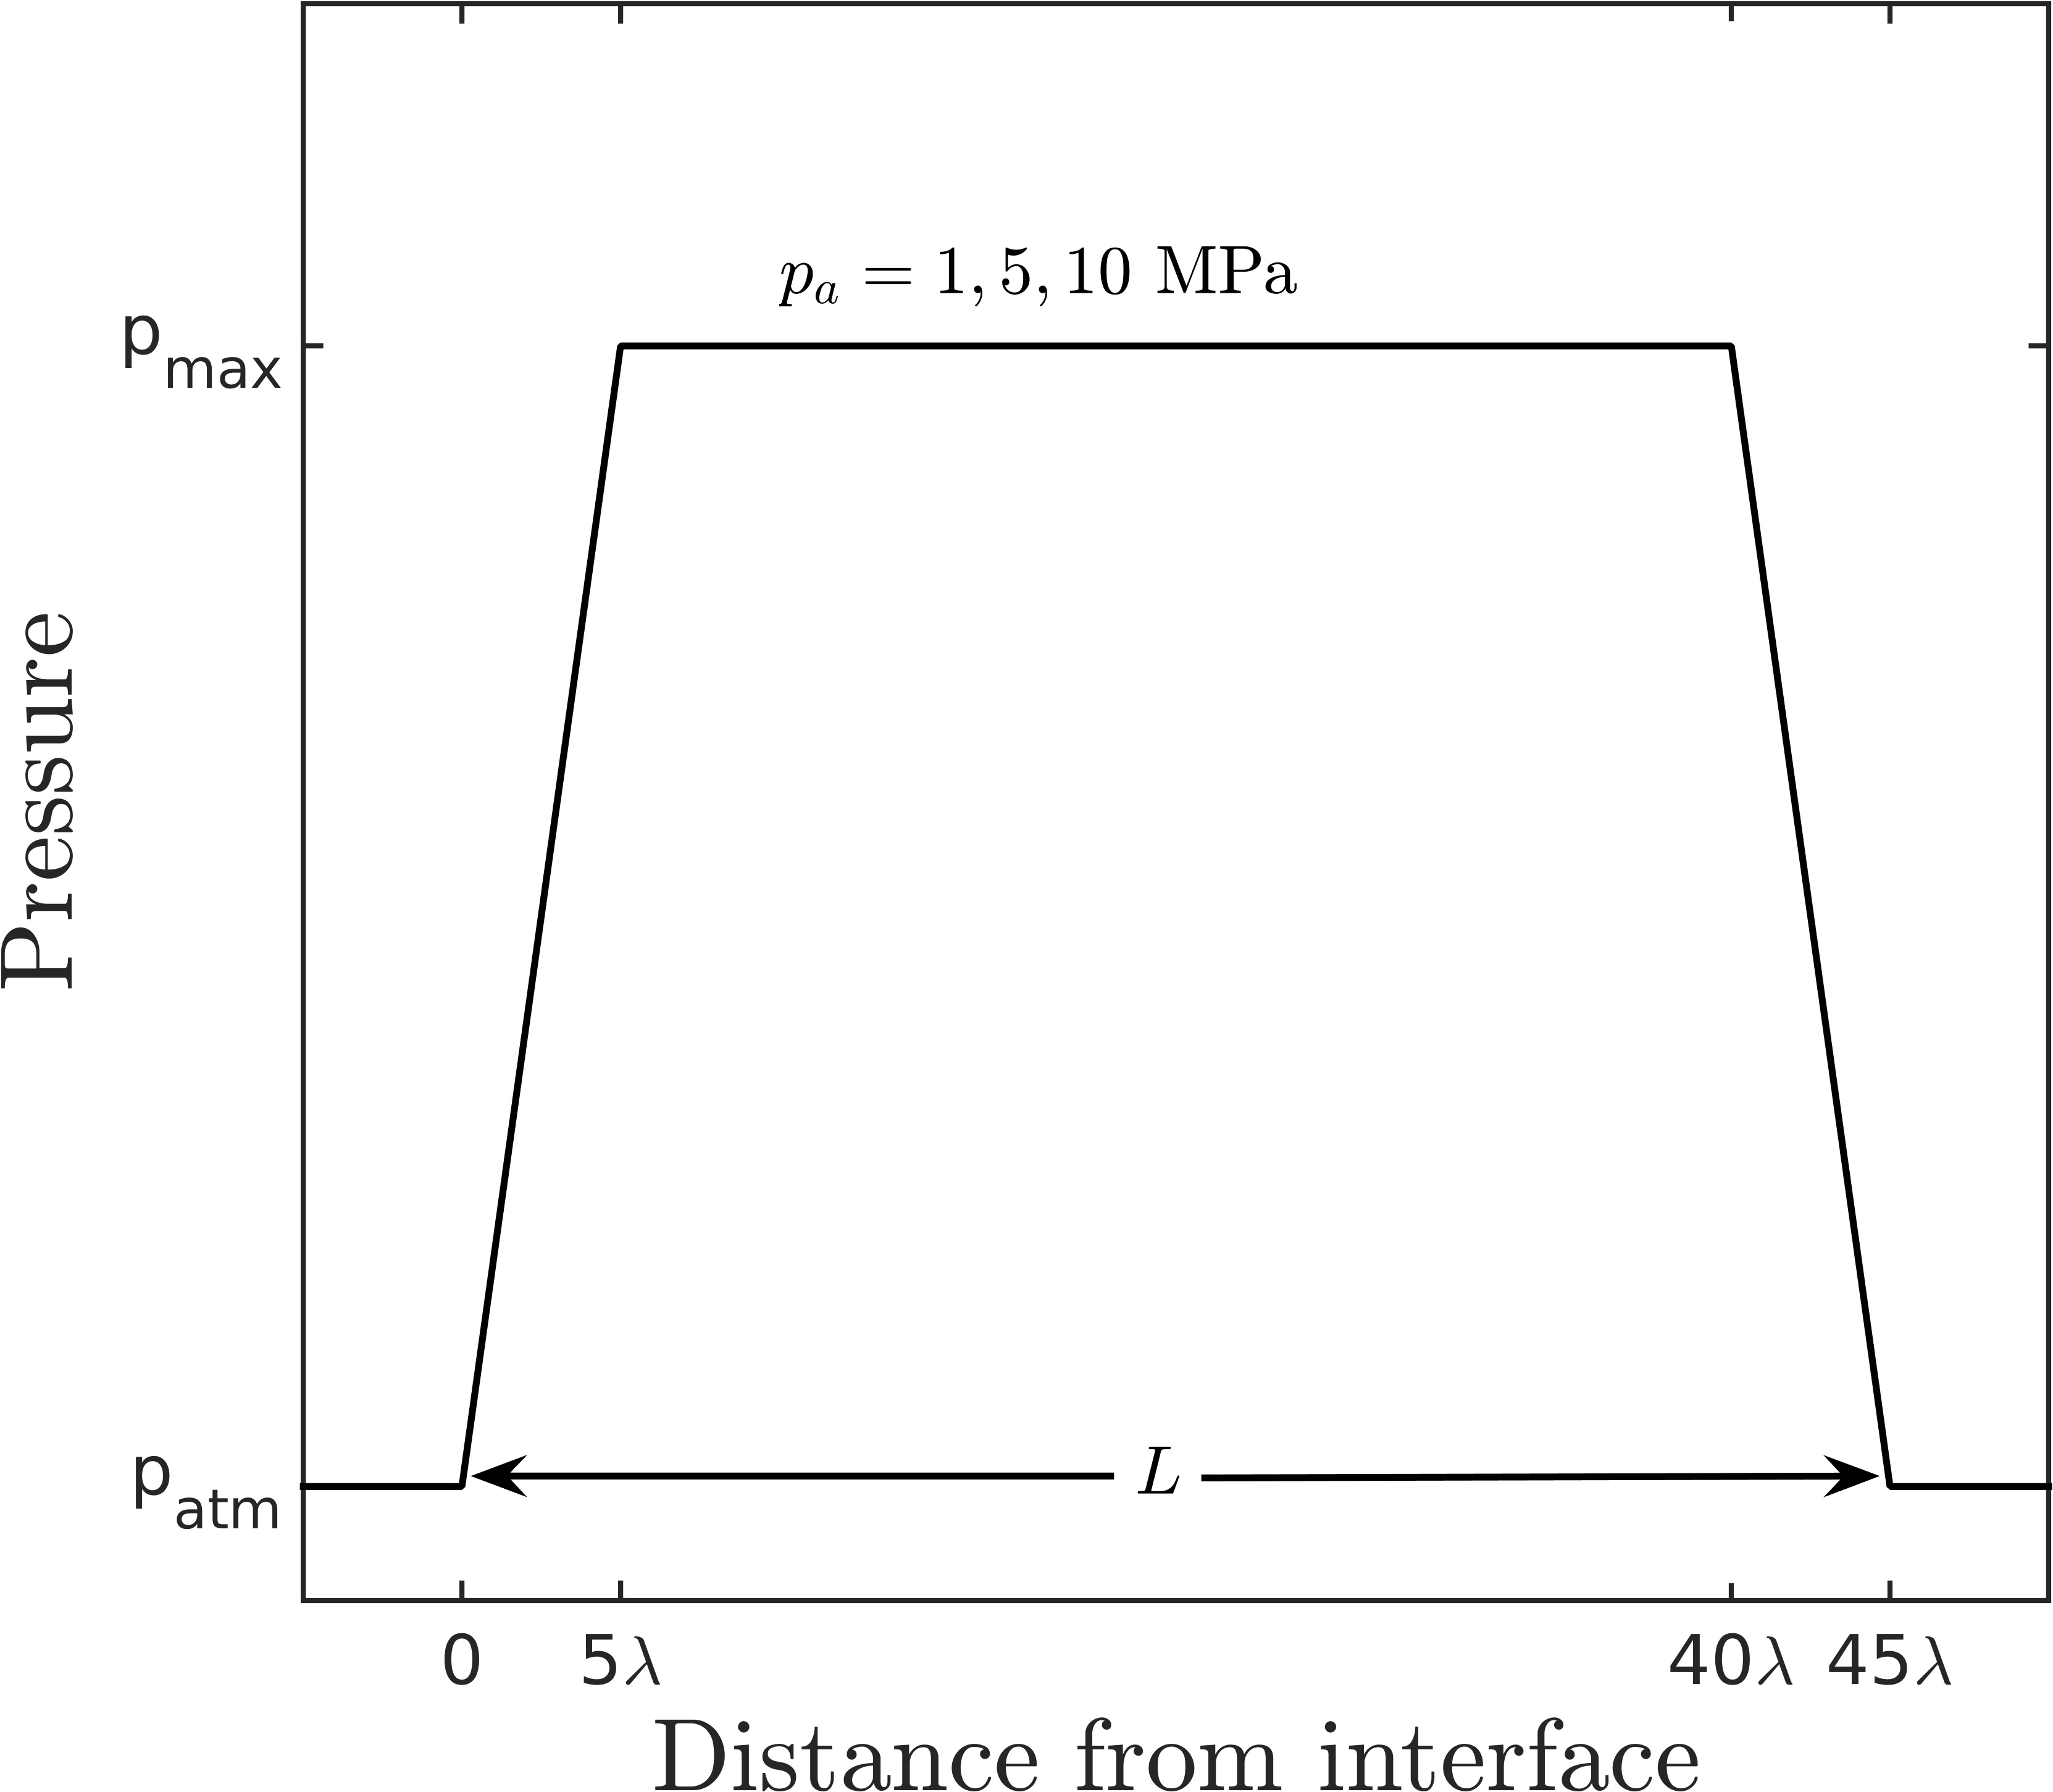
\includegraphics[width=0.47\textwidth]{./figs/lung_figs/p0_vs_y_labeled}%
  \caption[Trapezoidal wave]{The trapezoidal pressure wave prescribed
    as an in initial condition is shown as a function of distance from
    the interface.}%
  \label{fig:p0}
\end{figure}
% 
\subsection{Governing equations}
The governing equations describing the motivating problem of \ac{DUS}
of the lung are conservation of mass, momentum, and energy for a
compressible, viscoelastic material. The present work aims to
study the fundamental fluid physics of acoustically-accelerated,
perturbed liquid-gas interfaces, so we neglect elastic and viscous
effects. Hence We arrive at the Euler equations which we present here
for the case of fluid motion in two dimensions ($x,y$):
% 
\begin{subequations} \label{eq:euler}%
  \begin{align}% 
    \frac{\partial \rho}{\partial t} + \frac{\partial \left(\rho u\right)}{\partial x} + \frac{\partial \left(\rho v\right)}{\partial y} = 0,\\
    \frac{\partial \rho u}{\partial t} + \frac{\partial}{\partial x}\left( \rho u^2+p\right)  + \frac{\partial}{\partial y}\left( \rho uv\right) = 0,\\
    \frac{\partial \rho v}{\partial t} + \frac{\partial}{\partial x}\left( \rho uv\right)  + \frac{\partial}{\partial y}\left( \rho v^2+p\right) = 0,\\
    \frac{\partial E}{\partial t} + \frac{\partial}{\partial x}\left[u\left(E+p\right)\right] + \frac{\partial}{\partial y}\left[v\left(E+p\right)\right] = 0,
  \end{align}%
\end{subequations}%
% 
where $t$ is time, $\rho$ is density, $p$ is the pressure, $u$ and $v$
are the velocity components in the $x$ and $y$ directions
respectively, and $E$ is the total energy. We use the density and
sound speed of air at 300 K to nondimensionalize the system. It is
worth noting that the Euler equations are length scale invariant, and
thus no inherent physical length scale exists in the equations that we
solve. Hence all length scales hereafter will be considered relative
to an interface perturbation wavelength $\lambda$.

To close the system, we solve a stiffened equation of state which
relate the total energy to the pressure and velocity in the flow, such
that,
% 
\begin{align} \label{eq:stiffened_eos}%
  E=\frac{\rho\left(u^2+v^2\right)}{2} + \frac{p+\gamma B}{\gamma-1}.
\end{align}
% 
Here $B$ is a measure of liquid stiffness. For perfect gases, such as
is our treatment of air, $\gamma$ is the specific heats ratio and
$B=0$. The sound speed in our simulations is calculated based on the
following relationship, derived from the stiffened equation of state.
% 
\begin{align}
  c = \sqrt{\frac{\gamma\left(p+B\right)}{\rho}}.
\end{align}
% 
While physical diffusion is not considered in this setup, numerical
diffusion does occur at the water-air interface, creating a mixed
region between the two fluids. The numerical treatment of the
diffusion layer at the interface for the initial condition is such
that the density has an exponential profile \citep{Latini2007}, which
is used to get the mass fraction and molecular weight fields in the
mixed region. Which then used to determine the other material
parameters in the mixed region in a thermodynamically consistent
fashion.

To solve for
the material parameters in the mixed region and prevent spurious
pressure oscillations at the interface, two additional advection
equations are solved for $\gamma$ and $B$.
\begin{subequations} \label{usbe_lung_eosvar_advection}%
  \begin{align}% 
    \frac{\partial}{\partial t}\left(\frac{\gamma B}{\gamma-1}\right)+\vec{u}\frac{\partial}{\partial x}\left(\frac{\gamma B}{\gamma-1}\right) = 0,\\
    \frac{\partial}{\partial t}\left(\frac{1}{\gamma-1}\right)+\vec{u}\frac{\partial}{\partial x}\left(\frac{1}{\gamma-1}\right) = 0. 
  \end{align}%
\end{subequations}%
This implementation is consistent with the works of \cite{Abgrall1996,
  Shyue2001, Beig2015}. Details of the full numerical implementation
are explained by \cite{HenrydeFrahan2015}.
%
The dimensional and dimensionless values of each fluid property can be
found in tables \ref{tab:usbe_lung_dimensional_parameters} and
\ref{tab:usbe_lung_dimensionless_parameters} respectively.
% 
\begin{table}[bp]%
  \begin{center}
    \caption{Dimensional properties of air and water used in simulations.}
    \label{tab:usbe_lung_dimensional_parameters}%
    \begin{tabularx}{0.75\textwidth}{| X | X | X | X | X |}
      \hline
      & Density, $\rho^*$ (kg/m$^3$) & $\gamma$ & $B^*$ (Pa)  & $c^*$ (m/s) ($p$=$1$ atm) \\ \hline
      Air   & 1.18                        & 1.4      & 0         & 347.2     \\ \hline
      Water & 996                           & 5.5      & 492115000 & 1648.7     \\ \hline
      \multicolumn{5}{l}{\small $^*$ indicates dimensional parameter}
    \end{tabularx}
  \end{center}
\end{table}%
\begin{table}[bp]%
  \begin{center}
    \caption{Dimensionless properties of air and water used in simulations.}
    \label{tab:usbe_lung_dimensionless_parameters}%
    \begin{tabularx}{0.75\textwidth}{| X | X | X | X | X |}
      \hline
      & Density, $\rho$ & $\gamma$ & $B$ & $c$ \\ \hline
      Air   & 1                          & 1.4      & 0         & 1          \\ \hline
      Water & 846.6                      & 5.5      & 3469.1    & 4.75       \\ \hline
      \multicolumn{5}{l}{\small Parameters are nondimensionalized by the density and sound speed of air. }
    \end{tabularx}
  \end{center}
\end{table}
% 
\subsection{Numerical methods}%
\label{subsec:numerical_methods}%
To solve the governing equations, we implement a third-order accurate
\ac{DG} scheme in space and a fourth-order accurate, adaptive
Runge-Kutta method to march forward in time
\citep{HenrydeFrahan2015}. Roe solver is used to calculate flux in an
out of each cell in a way that handles discontinuities and keeps the
interface sharp. As previously stated, the computational domain width
($x$-direction) is $\lambda$. The domain length ($y$-direction) is
80$\lambda$. The grid resolution is 100 points per $\lambda$ unless
otherwise stated. To minimize artificial reflections, we use inflow
and outflow boundary conditions at the top and bottom of the domain,
and implement geometric grid stretching in the vertical direction for
the top and bottom-most 10$\lambda$ segments of the grid. Periodic
boundary conditions are used at the left and right edges of the
domain.

%%% Local Variables:
%%% mode: latex
%%% TeX-master: "../main"
%%% End:

\section{Results, analysis, and discussion}%
\label{sec:results}%
%
In this section we present the results of the numerical experiments
and compare them to our analysis. We focus specifically on the
relationship between circulation and interface dynamics.
%
%
\subsection{Qualitative observations of the interface response to the $p_a=10$ MPa trapezoidal wave}
\label{subsec:Qualitative}
To provide a qualitative understanding of the underlying physics, we
consider our reference case in which a $p_a=10$ MPa trapezoidal wave
(See Figure \ref{fig:p0}) impinges on the water-air interface. Nearly
all of the acoustic energy is reflected back into the
water as a tension wave due lower acoustic impedance of the second
fluid. The transmitted compression wave is weakly focused due to the sound
speed mismatch across the curved interface perturbation. These
reflected and transmitted waves dissipate at the inflow and outflow
boundaries.
%
\begin{figure}[h] 
  \centering
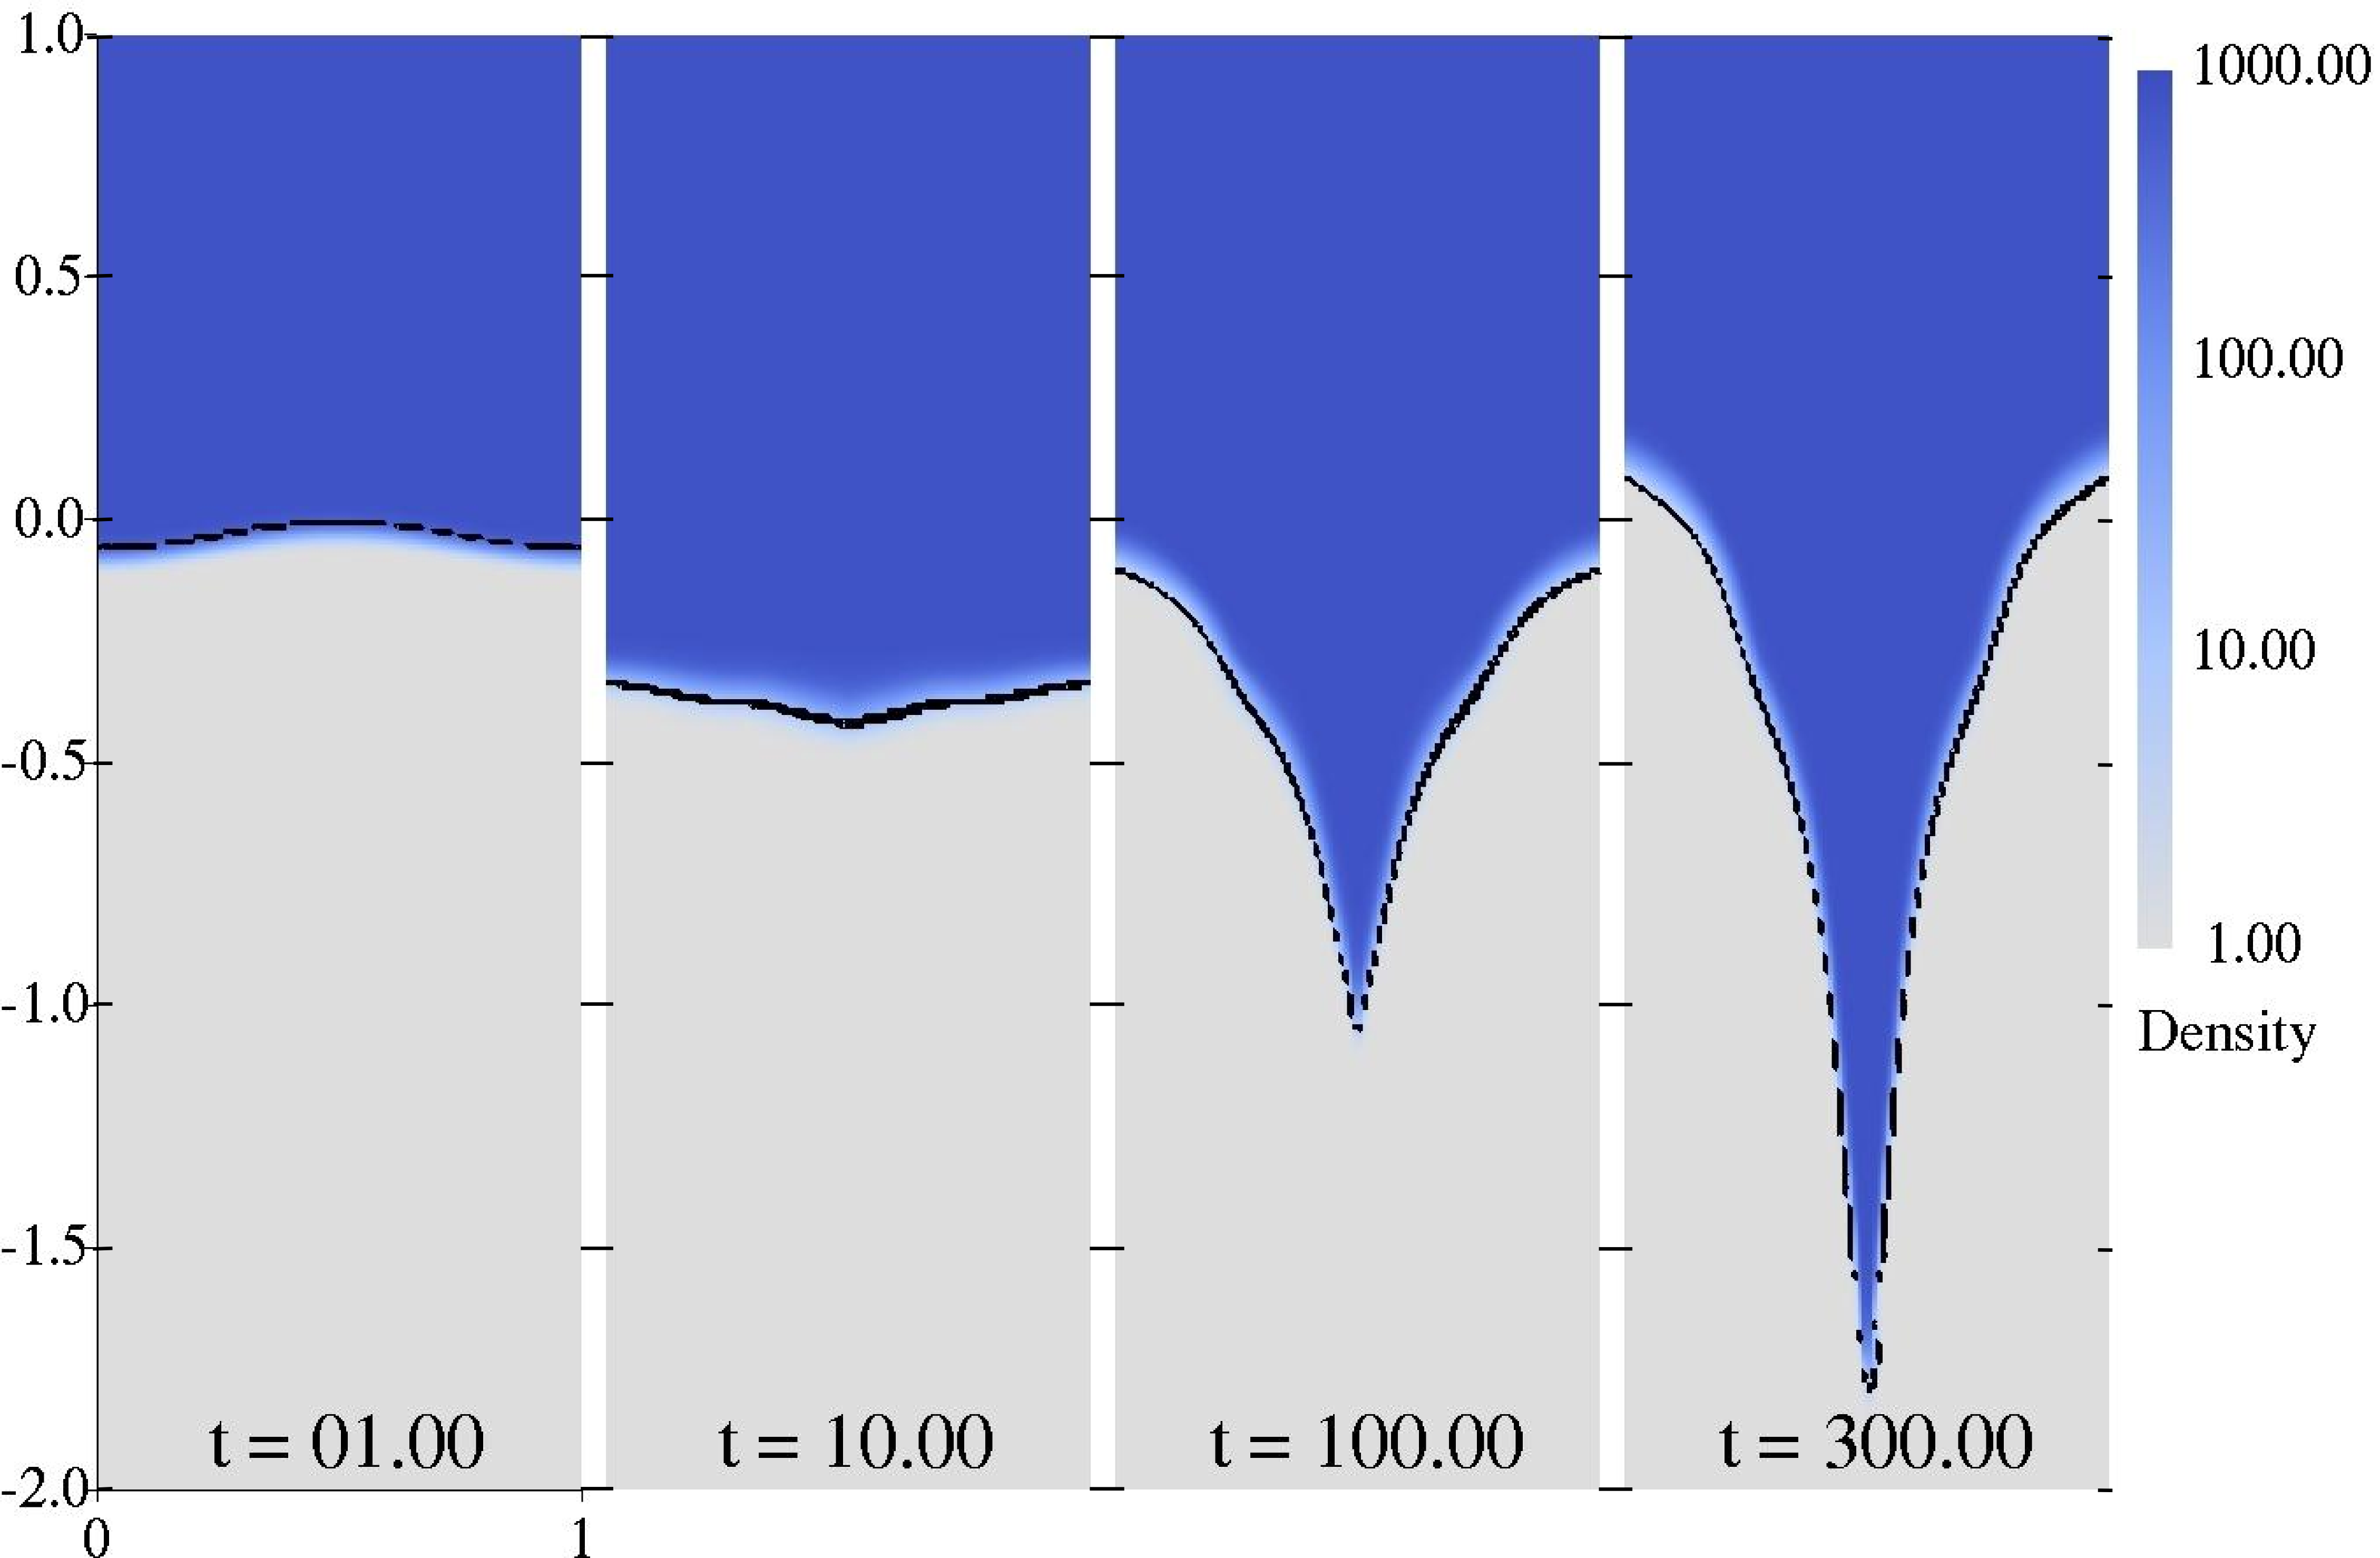
\includegraphics[width=0.9\textwidth]{./figs/lung_figs/snapshots_density_t1}
%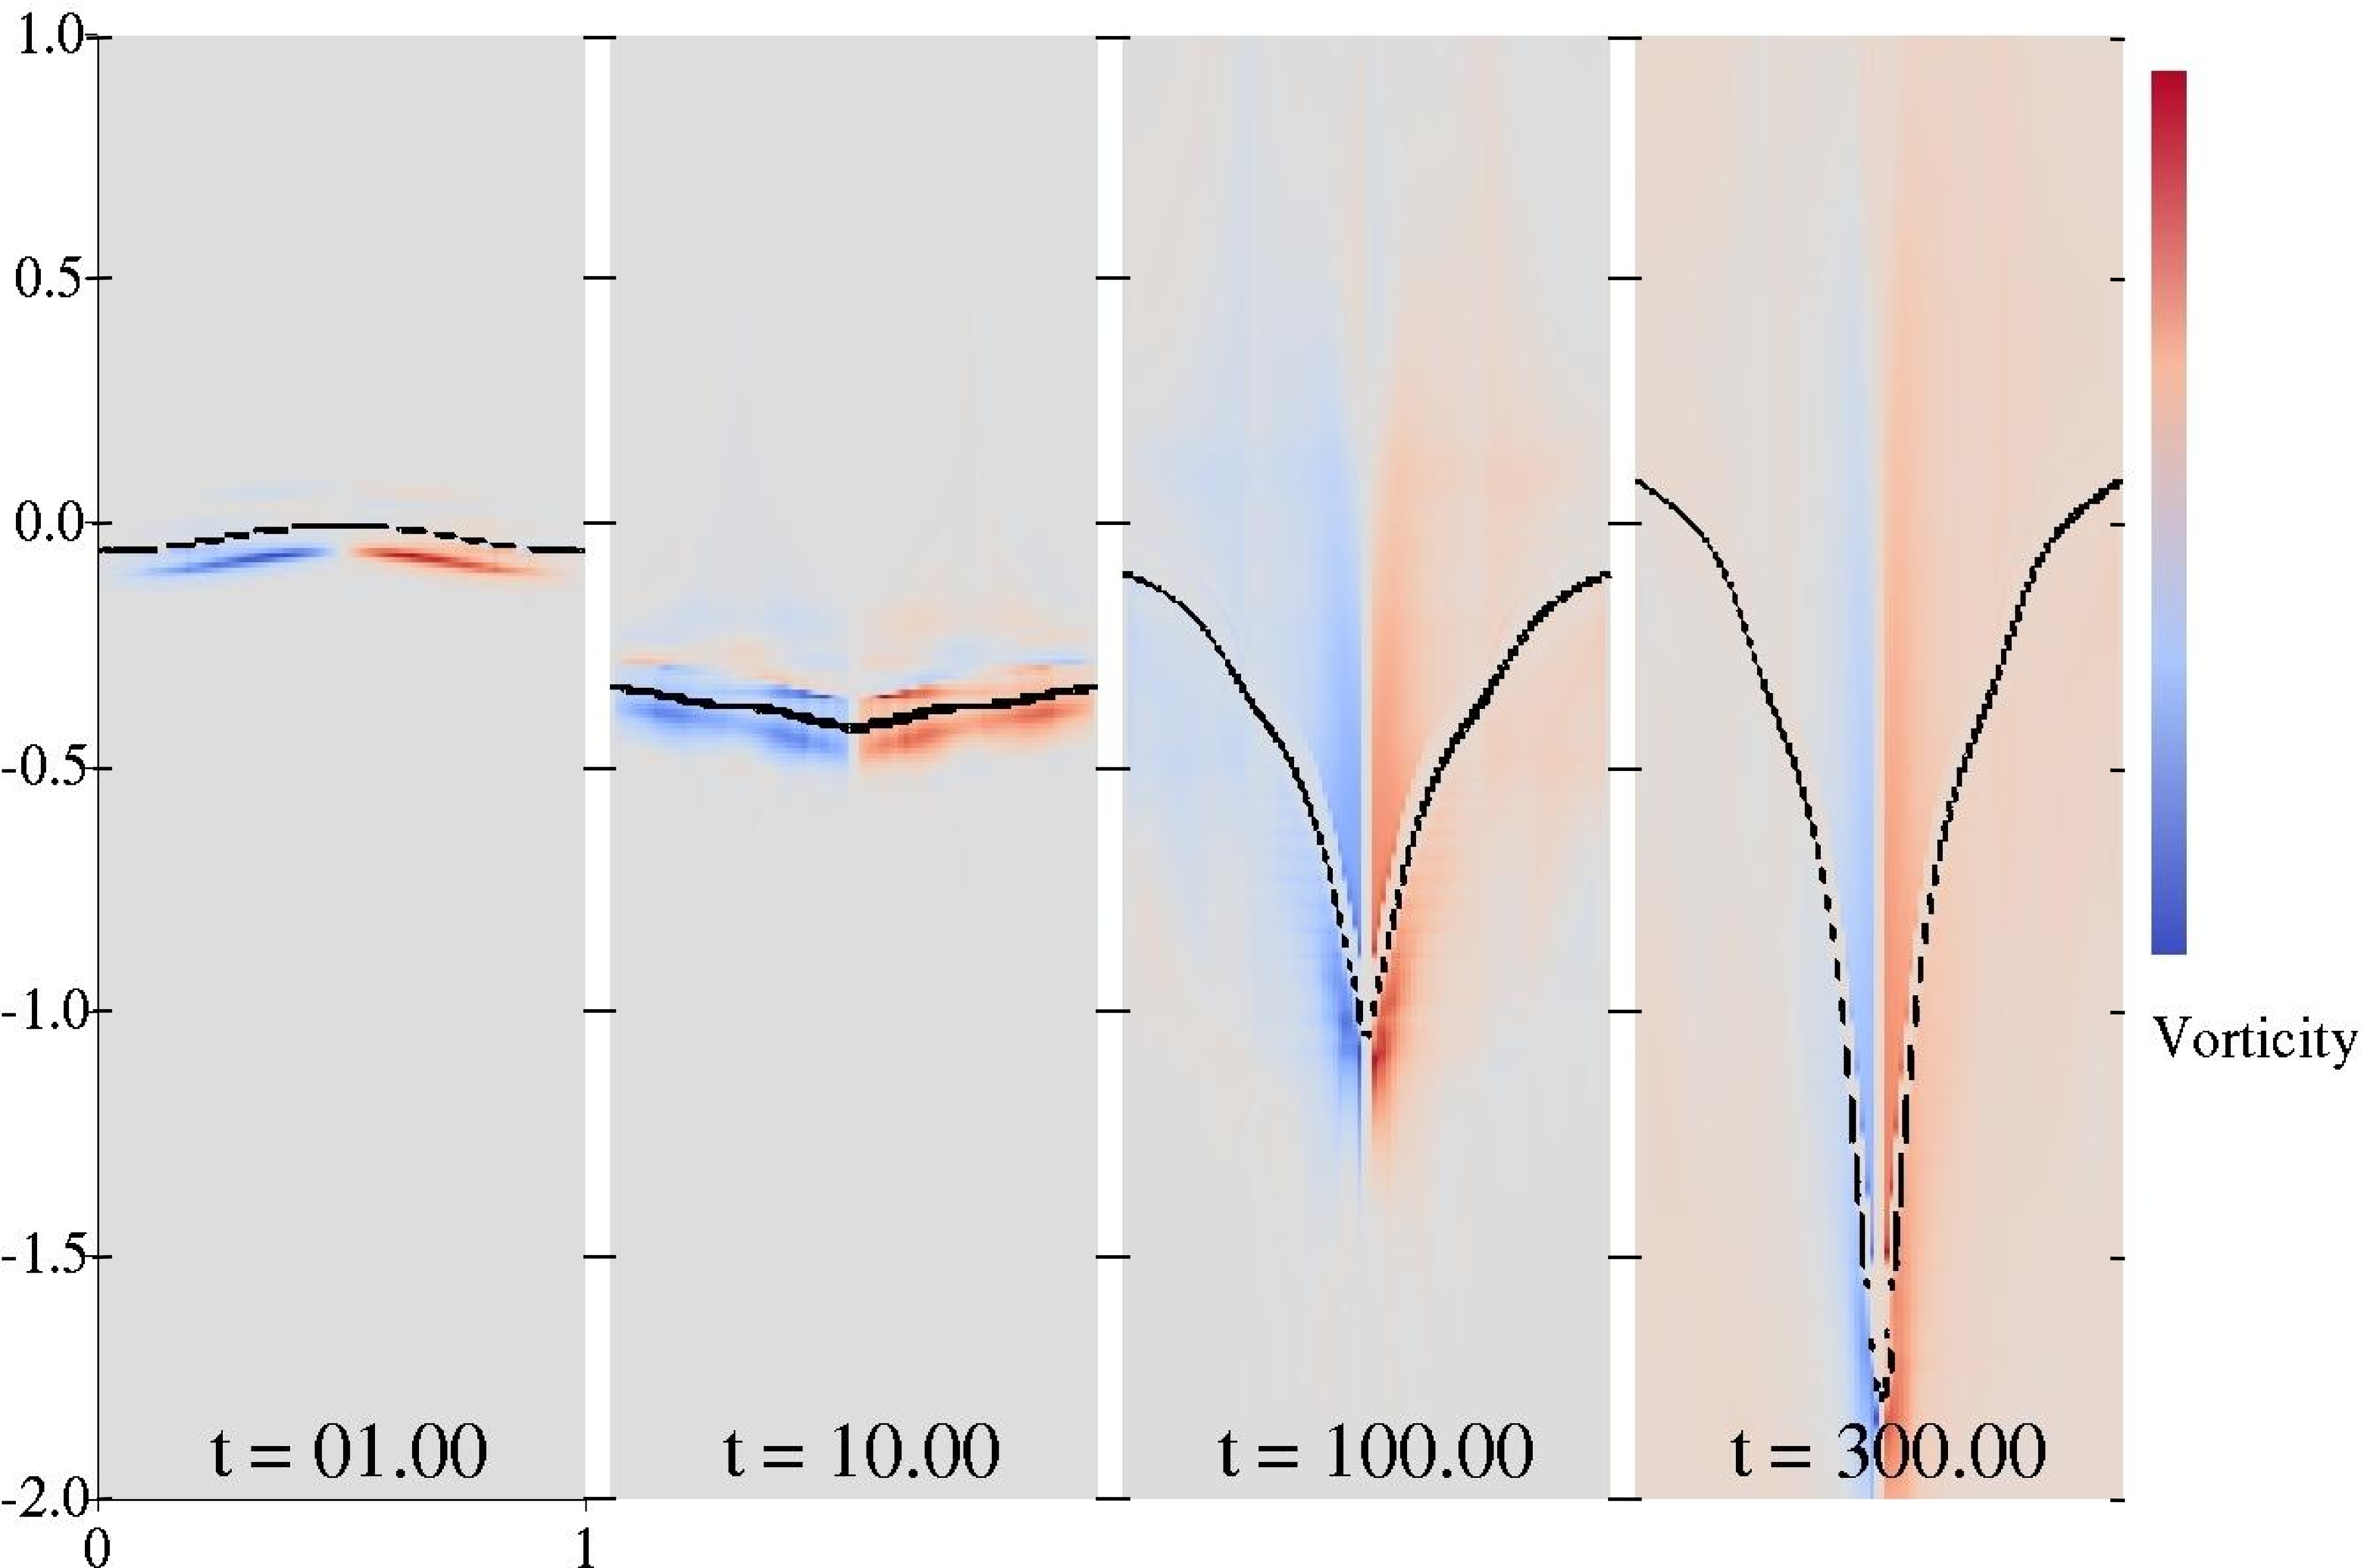
\includegraphics[width=0.9\textwidth]{./figs/lung_figs/snapshots_vorticity_t1}
\caption[The evolution of the acoustically perturbed interface]
{Surface plots of density throughout the evolution of the interface,
  at $t=1, 10, 100, 300$, for the $10$ MPa trapezoidal wave
  case. Areas of high density (i.e., water) are indicated in dark
  blue. Areas of low density (i.e., air) are indicated in white.}
  \label{fig:interface_snapshots}
\end{figure}
%
To illustrate the evolution of the interface, Figure
\ref{fig:interface_snapshots} contains color plots of the density
during the compression-interface interaction $(t=1)$, immediately
after the wave leaves the interface $(t=10)$, and at late times
$(t=100, 300)$. Contours of 0.5 volume fraction of water are indicated
in black on both plots. The initially smooth interface perturbation
grows from a smooth sinusoid to a sharp point at late times.


\section{OLD}
%---------------------------------------------------------------------

 vorticity (Bottom) fields at different instances in
the flow's evolution. Areas of high density (i.e., water) are dark
blue and areas of low density (i.e., air) are light-blue. On the
vorticity contours, counterclockwise (positive) vorticity is red, and
clockwise (negative) vorticity is blue. The purpose of the vorticity
plots is only to show the location and direction of vorticity at each
time. For sake of visualization, the range of the vorticity color
scale changes at each time slice because the vorticity spreads over
time. Hence the vorticity magnitudes are not shown here.  

The initially smooth interface perturbation grows from a smooth
sinusoid to a sharp spike at late time.  vorticity is heavily
concentrated in the air. At $t=1$, the compression-interface
interaction has nearly completed and 97\% of the total circulation in
the left or right half domain exists in fluid with volume fraction
$\alpha<0.5$. This is qualitatively consistent with our analysis. As
time progresses, it can be seen that the vorticity disperses
throughout the domain, but remains concentrated around the interface
and the vertical center of the domain.

To more closely exam the interface and circulation dynamics associated
with the compression wave-interface interaction, Figure
\ref{fig:trapz10_circ_interface} shows the early-time histories of the
interface amplitude $a(t)$ and half-domain circulation $\Gamma$. We
have labeled the times at which different portions of the incoming
wave encounter the interface as $t_{1-4}$, denoted with black
$\bs{\times}$s along the curves in these figures and those
hereafter. From $t_1=0^+$ to $t_2$ the compression wave encounters the
interface. During this interaction the perturbation amplitude
decreases, and the right half-domain circulation $\Gamma$ rises
sharply. At $t_2\approx1.1$, the pressure reaches its maximum
amplitude, $p_a=10$ MPa, and remains constant until $t_3$. We note
that at $\overline{a(t_{1-2})}/a_0\approx0.96$, suggesting that the
static interface assumption made in our vorticity generation order of
magnitude analysis was reasonable. The interface amplitude continues
to decrease and the half-domain circulation $\Gamma$ stops its rapid
growth and changes little during this static elevated pressure period,
until the expansion wave hits at $t_3$. At $t\approx 5.0$, the
perturbation undergoes a phase inversion and begins to grow, as is
observed for the heavy-light interface Richtmyer-Meshkov problem. At
$t_3\approx8.5$ the expansion wave first hits the interface. The
perturbation amplitude continues to grow, and $\Gamma$ increases
sharply again. At $t_4\approx9.7$ the acoustic wave has finished
traversing the interface, and atmospheric pressure is resumed. The
perturbation amplitude $a_0$ continues to grow long after the
wave-interface interaction has finished.
%
\begin{figure}[h] 
  \centering
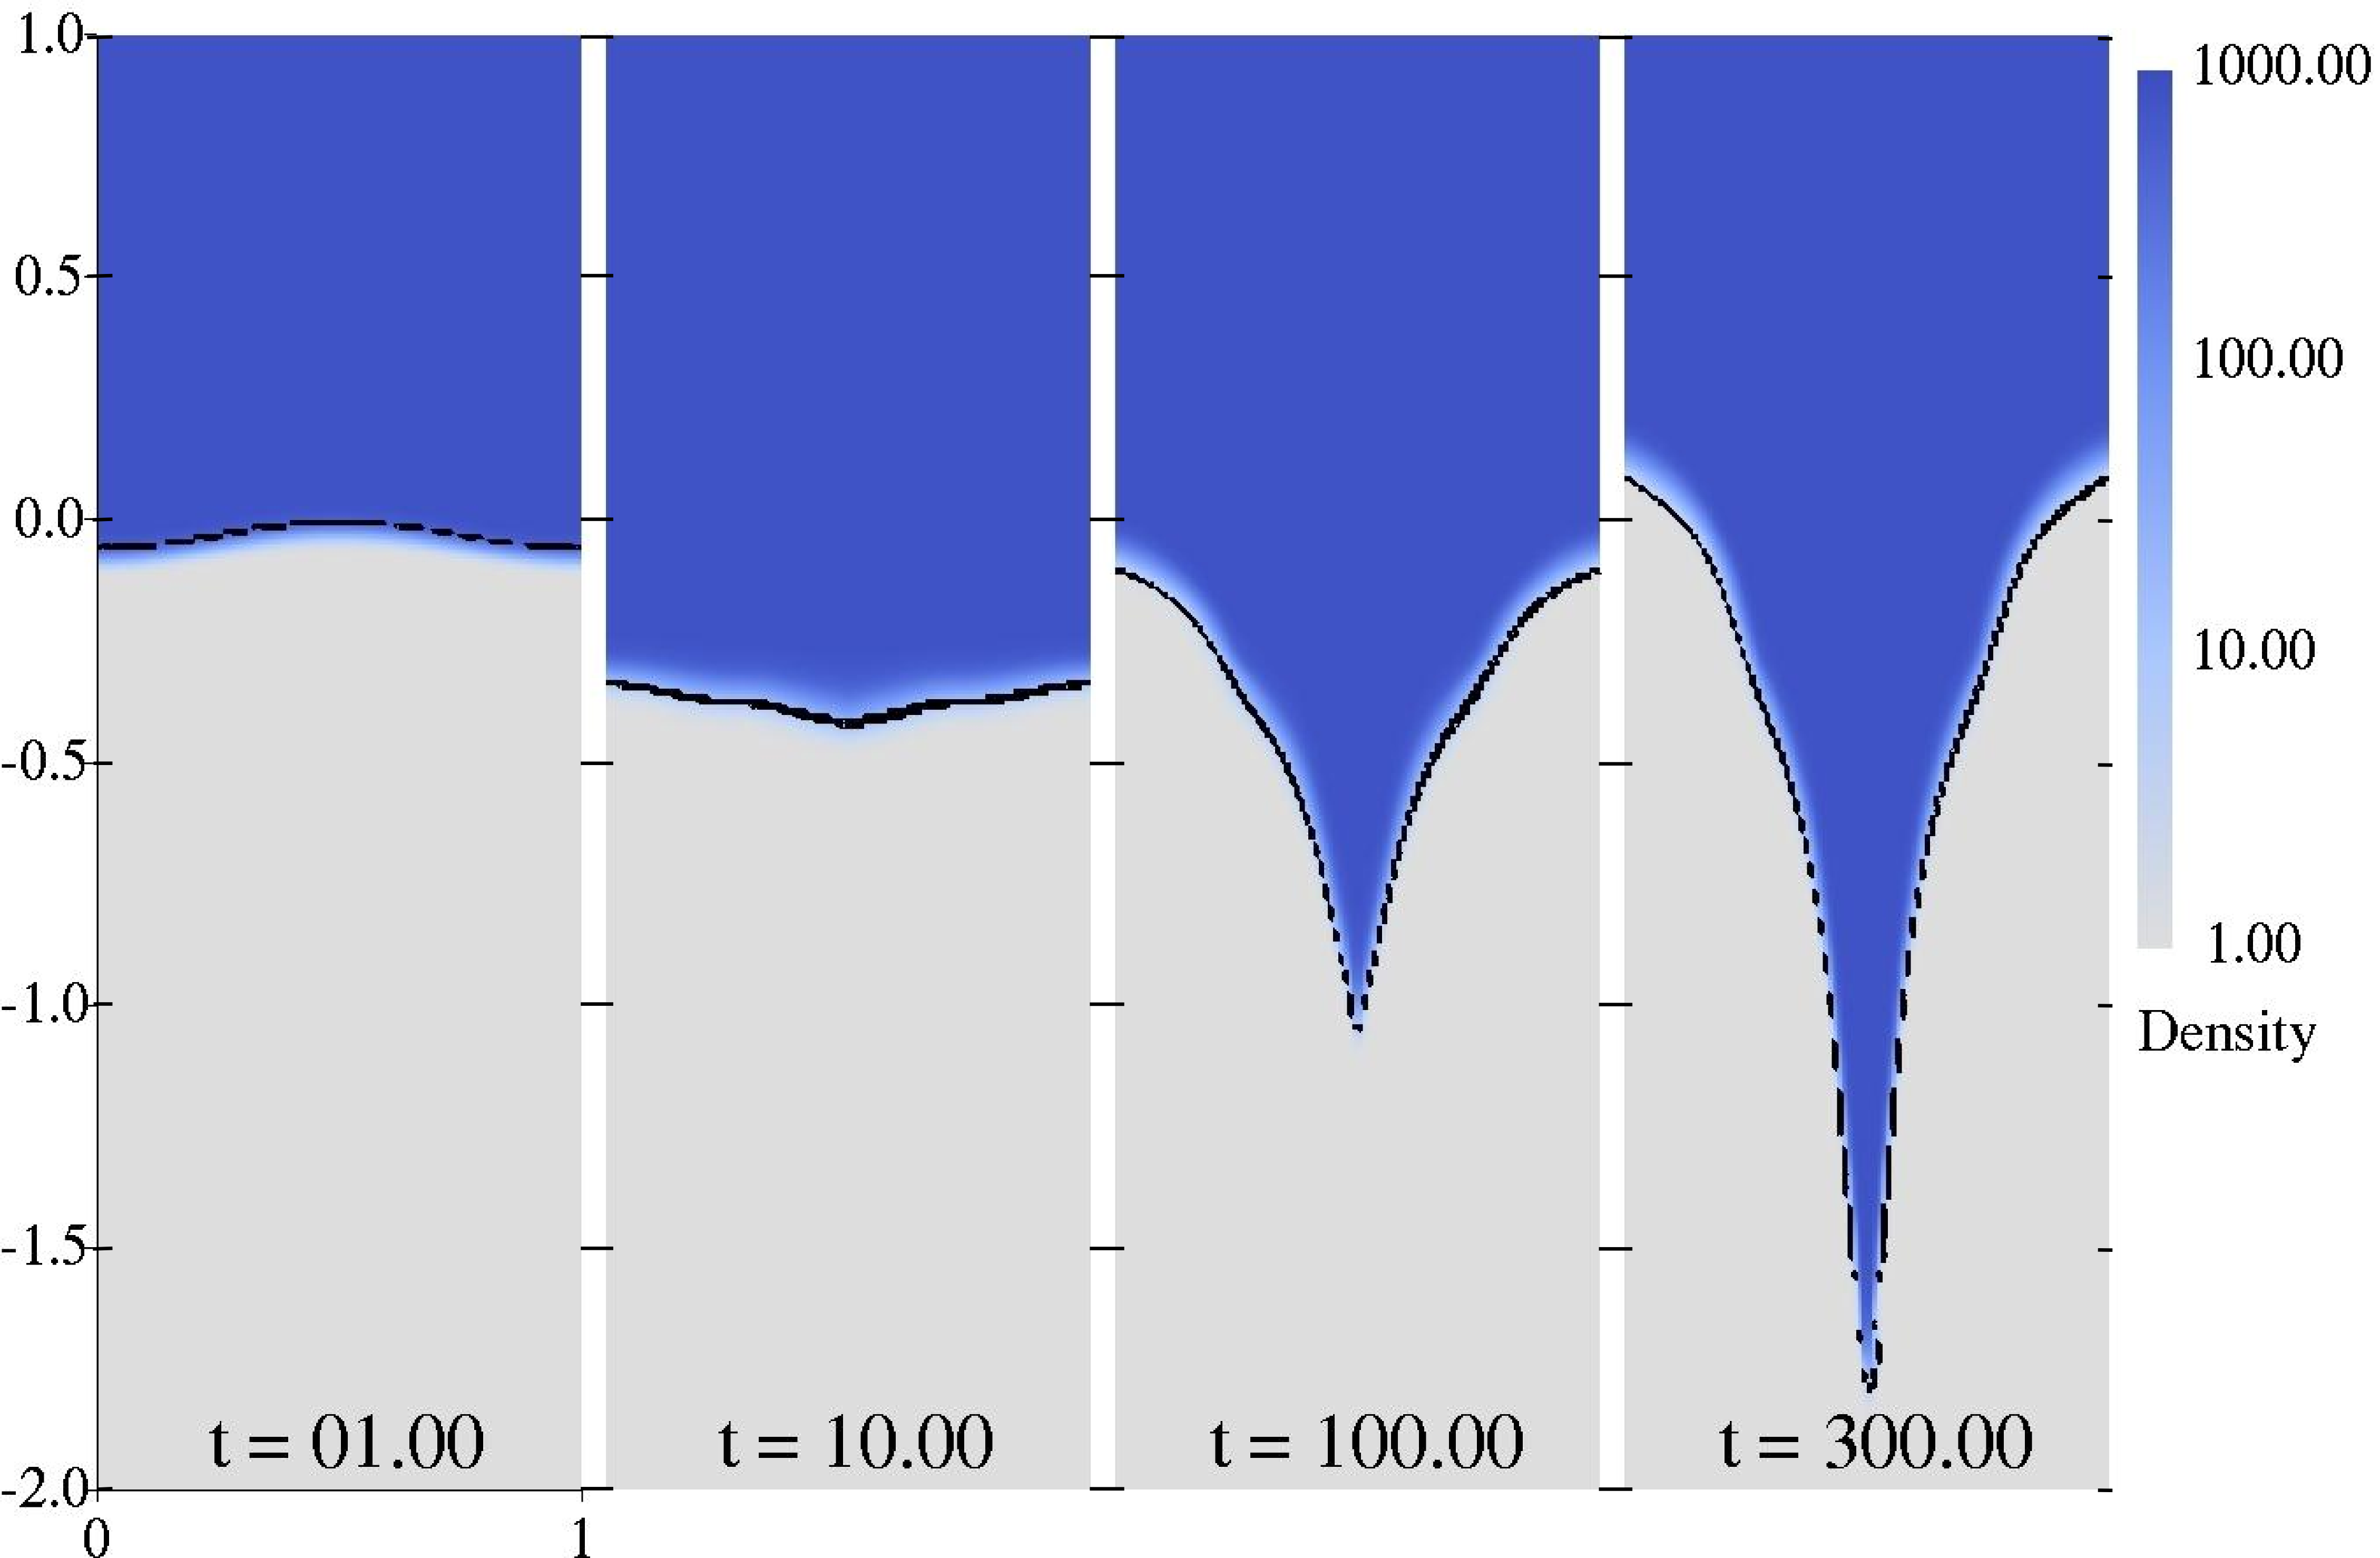
\includegraphics[width=0.9\textwidth]{./figs/lung_figs/snapshots_density_t1}
%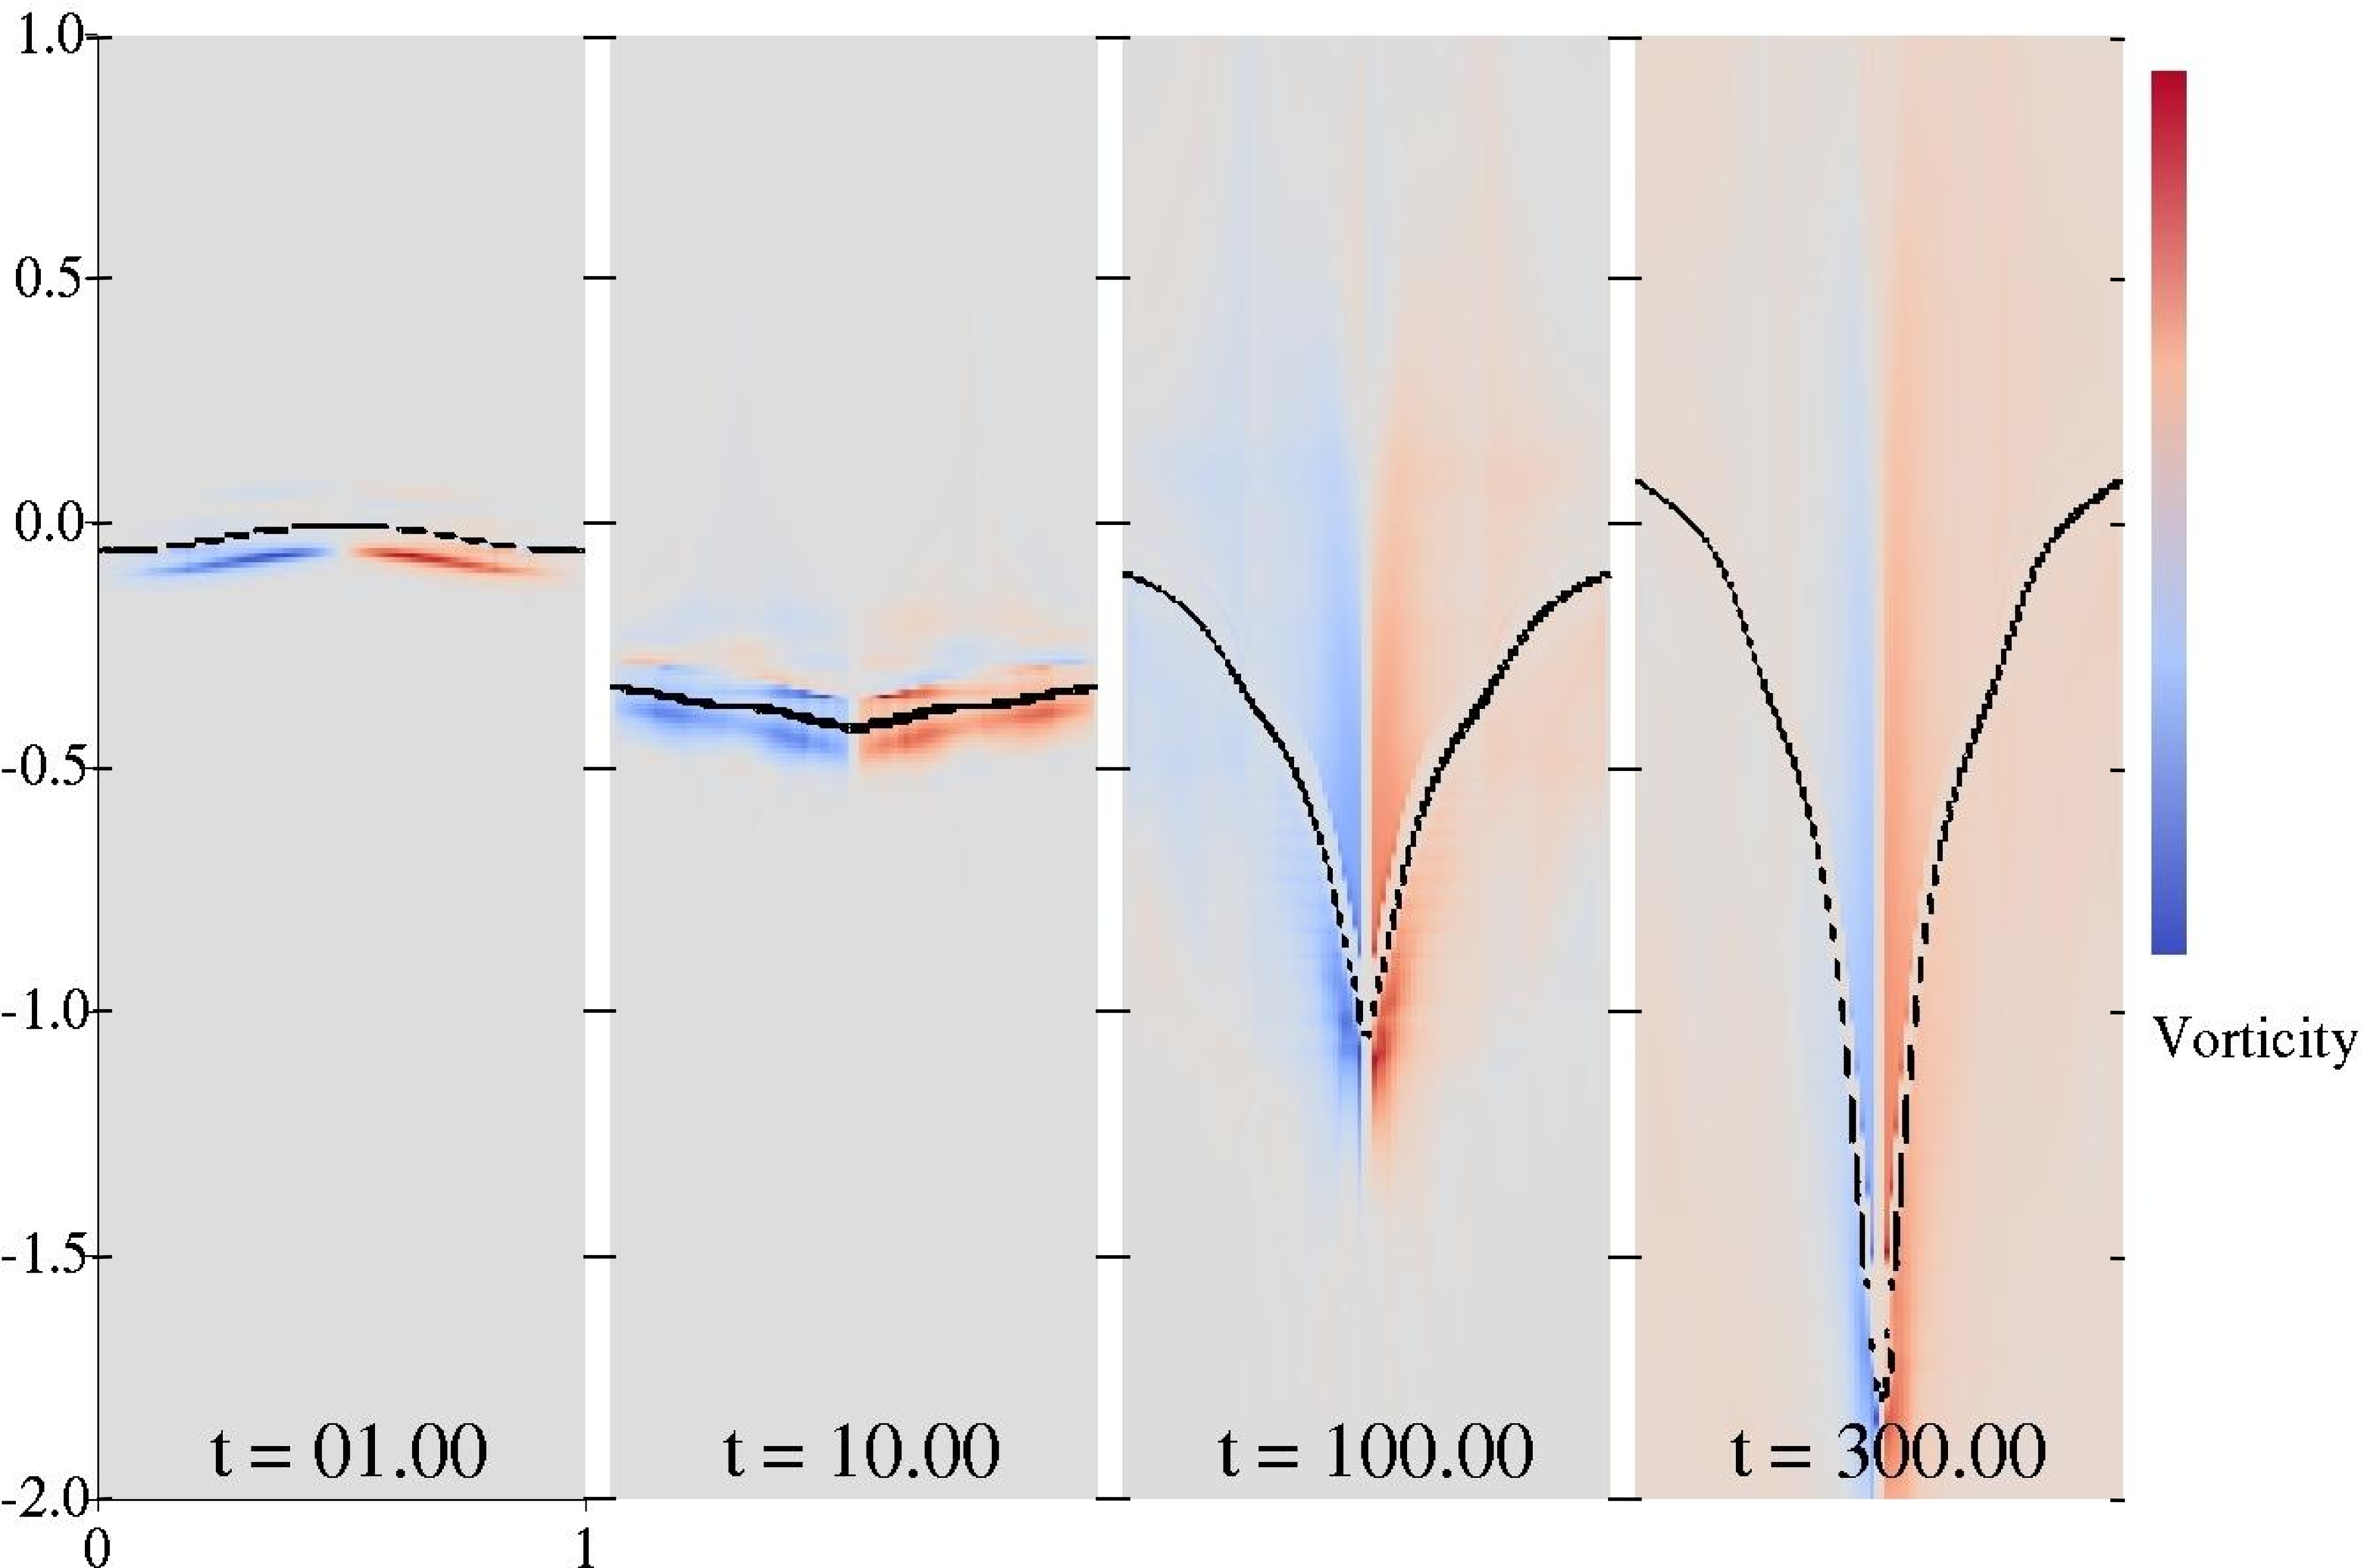
\includegraphics[width=0.9\textwidth]{./figs/lung_figs/snapshots_vorticity_t1}
\caption[The evolution of the acoustically perturbed interface and vorticity field]{Surface plots of density (Top) and vorticity (Bottom)
  throughout the evolution of the interface for the $10$ MPa
  trapezoidal wave case. Areas of high density (i.e., water) are
indicated in dark blue. Areas of low density (i.e., air) are indicated
in white.  Positive (counterclockwise) vorticity is indicated in red,
and negative (clockwise) vorticity can be seen in blue.}
  \label{fig:interface_snapshots}
\end{figure}
%
\begin{figure}[h] 
  \centering
  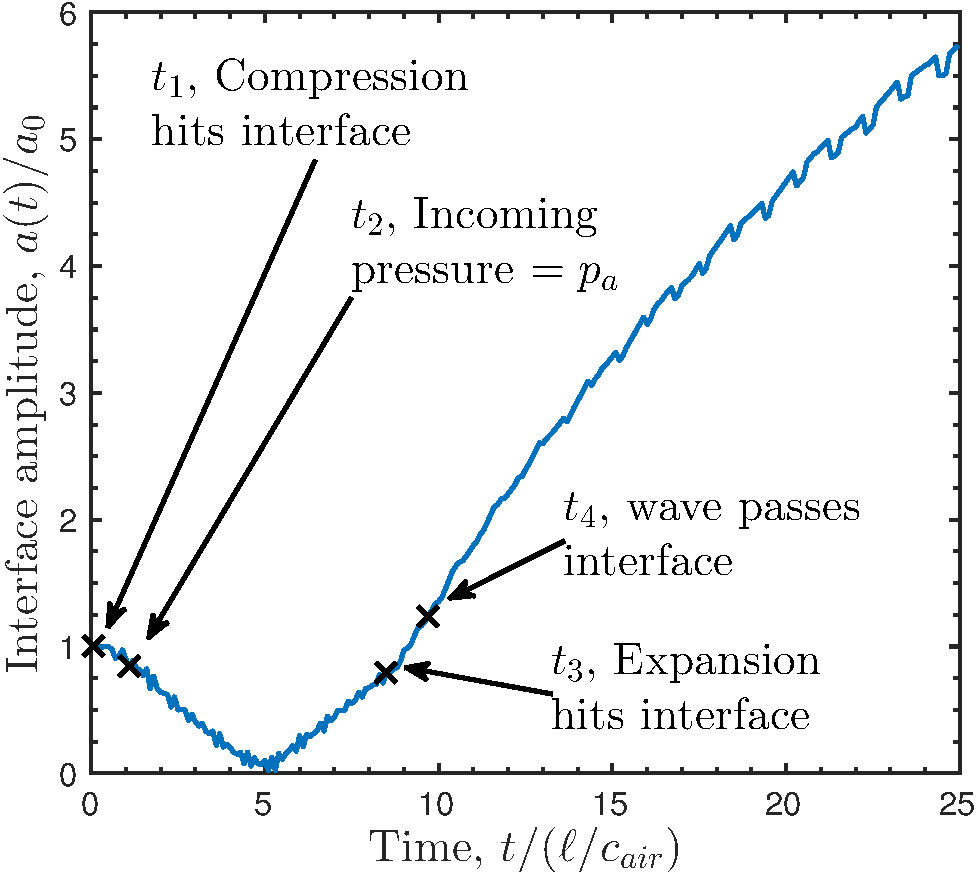
\includegraphics[width=0.48\textwidth]{./figs/lung_figs/trapz10_intf_schematic}
  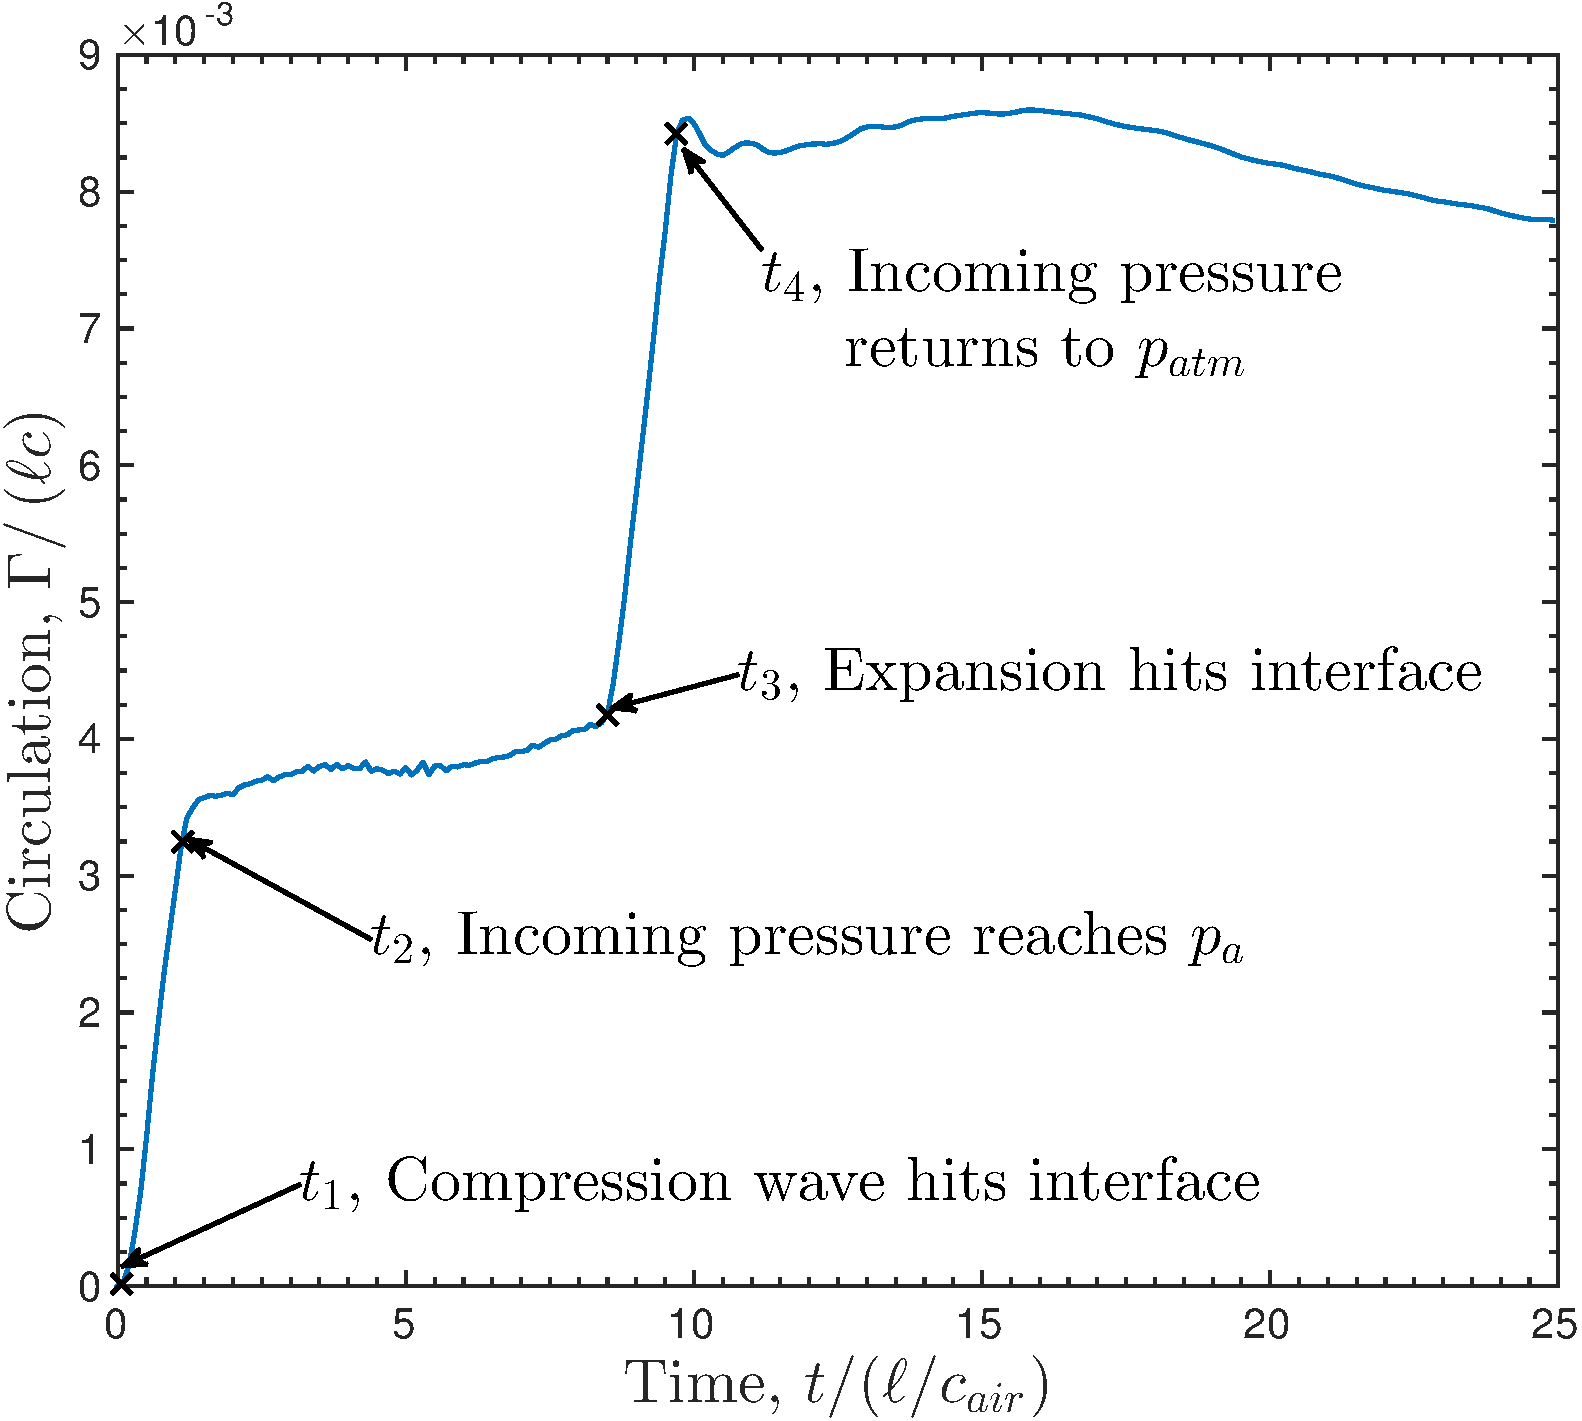
\includegraphics[width=0.48\textwidth]{./figs/lung_figs/trapz10_circ_schematic}
  \caption[The interface amplitude and circulation histories for the $10$ MPa trapezoidal wave]{The interface amplitude (left) and circulation (right)
    histories corresponding to the $10$ MPa trapezoidal waves are
    shown for $t\leq25$. Indicated times, $t_{1-4}$, are the times at
    which different stages of the incoming trapezoidal pressure wave
    shown in Figure \ref{fig:p0} first encounter the interface.}
  \label{fig:trapz10_circ_interface}
\end{figure}
%
%
\subsubsection{Dependence on acoustic wave amplitude}%
\label{subsubsec:amplitude_dependence}%
To investigate the dependence of the dynamics on the trapezoidal wave
amplitude, we compare results for $p_a=1$, $5$, and $10$ MPa while
keeping the initial lengths of the wave $L$ and the rise and fall
$\Delta L_a$ constant such that $p_a$ scales linearly with the
acoustic pressure gradient. Figure
\ref{fig:trapz_circ_interface_early}, illustrates the interface
amplitude and $p_a$-normalized circulation histories for $t\leq25$,
during and shortly after the wave-interface interaction. Black
$\bs{\times}$s along the curves indicate $t_{1-4}$, described
previously in Subsection \label{subsec:Qualitative}. During the
interaction between the interface and the compression wave, the rate
at which the perturbation amplitude decreases is greater for higher
amplitude waves. The circulation deposited during this period scales
linearly with $p_a$ as is consistent with baroclinically-generated
circulation based on our analysis. For the $10$ MPa wave, the phase of
the interface inverts at, before the expansion hits, causing
circulation deposited by the expansion to have the same sign as that
deposited by the compression. For the $1$ and $5$ MPa waves interface
phase inversion occurs after the expansion and consequently deposits
circulation opposite that of the compression wave.

Figure \ref{fig:trapz_circ_interface_loglog} \hl{(update this figure)}
shows the interface amplitude and circulation histories for $5$ and
$10$ MPa trapezoidal wave cases for $0 \leq t\leq 1000$. The
perturbation amplitude history is plotted on logarithmically-scaled
axes. For both waves, the slope of the perturbation amplitude is
approximately $0.60$ long after the waves have left the
interface. This is slightly higher than the 0.5 slope predicted by
scaling law \eqref{eq:intf_circ_scaling}. The results for the $1$ MPa
trapezoidal wave were not included because interface evolved too
slowly to obtain useful data given the computational resources available.
%
\begin{figure}[h] 
  \centering
  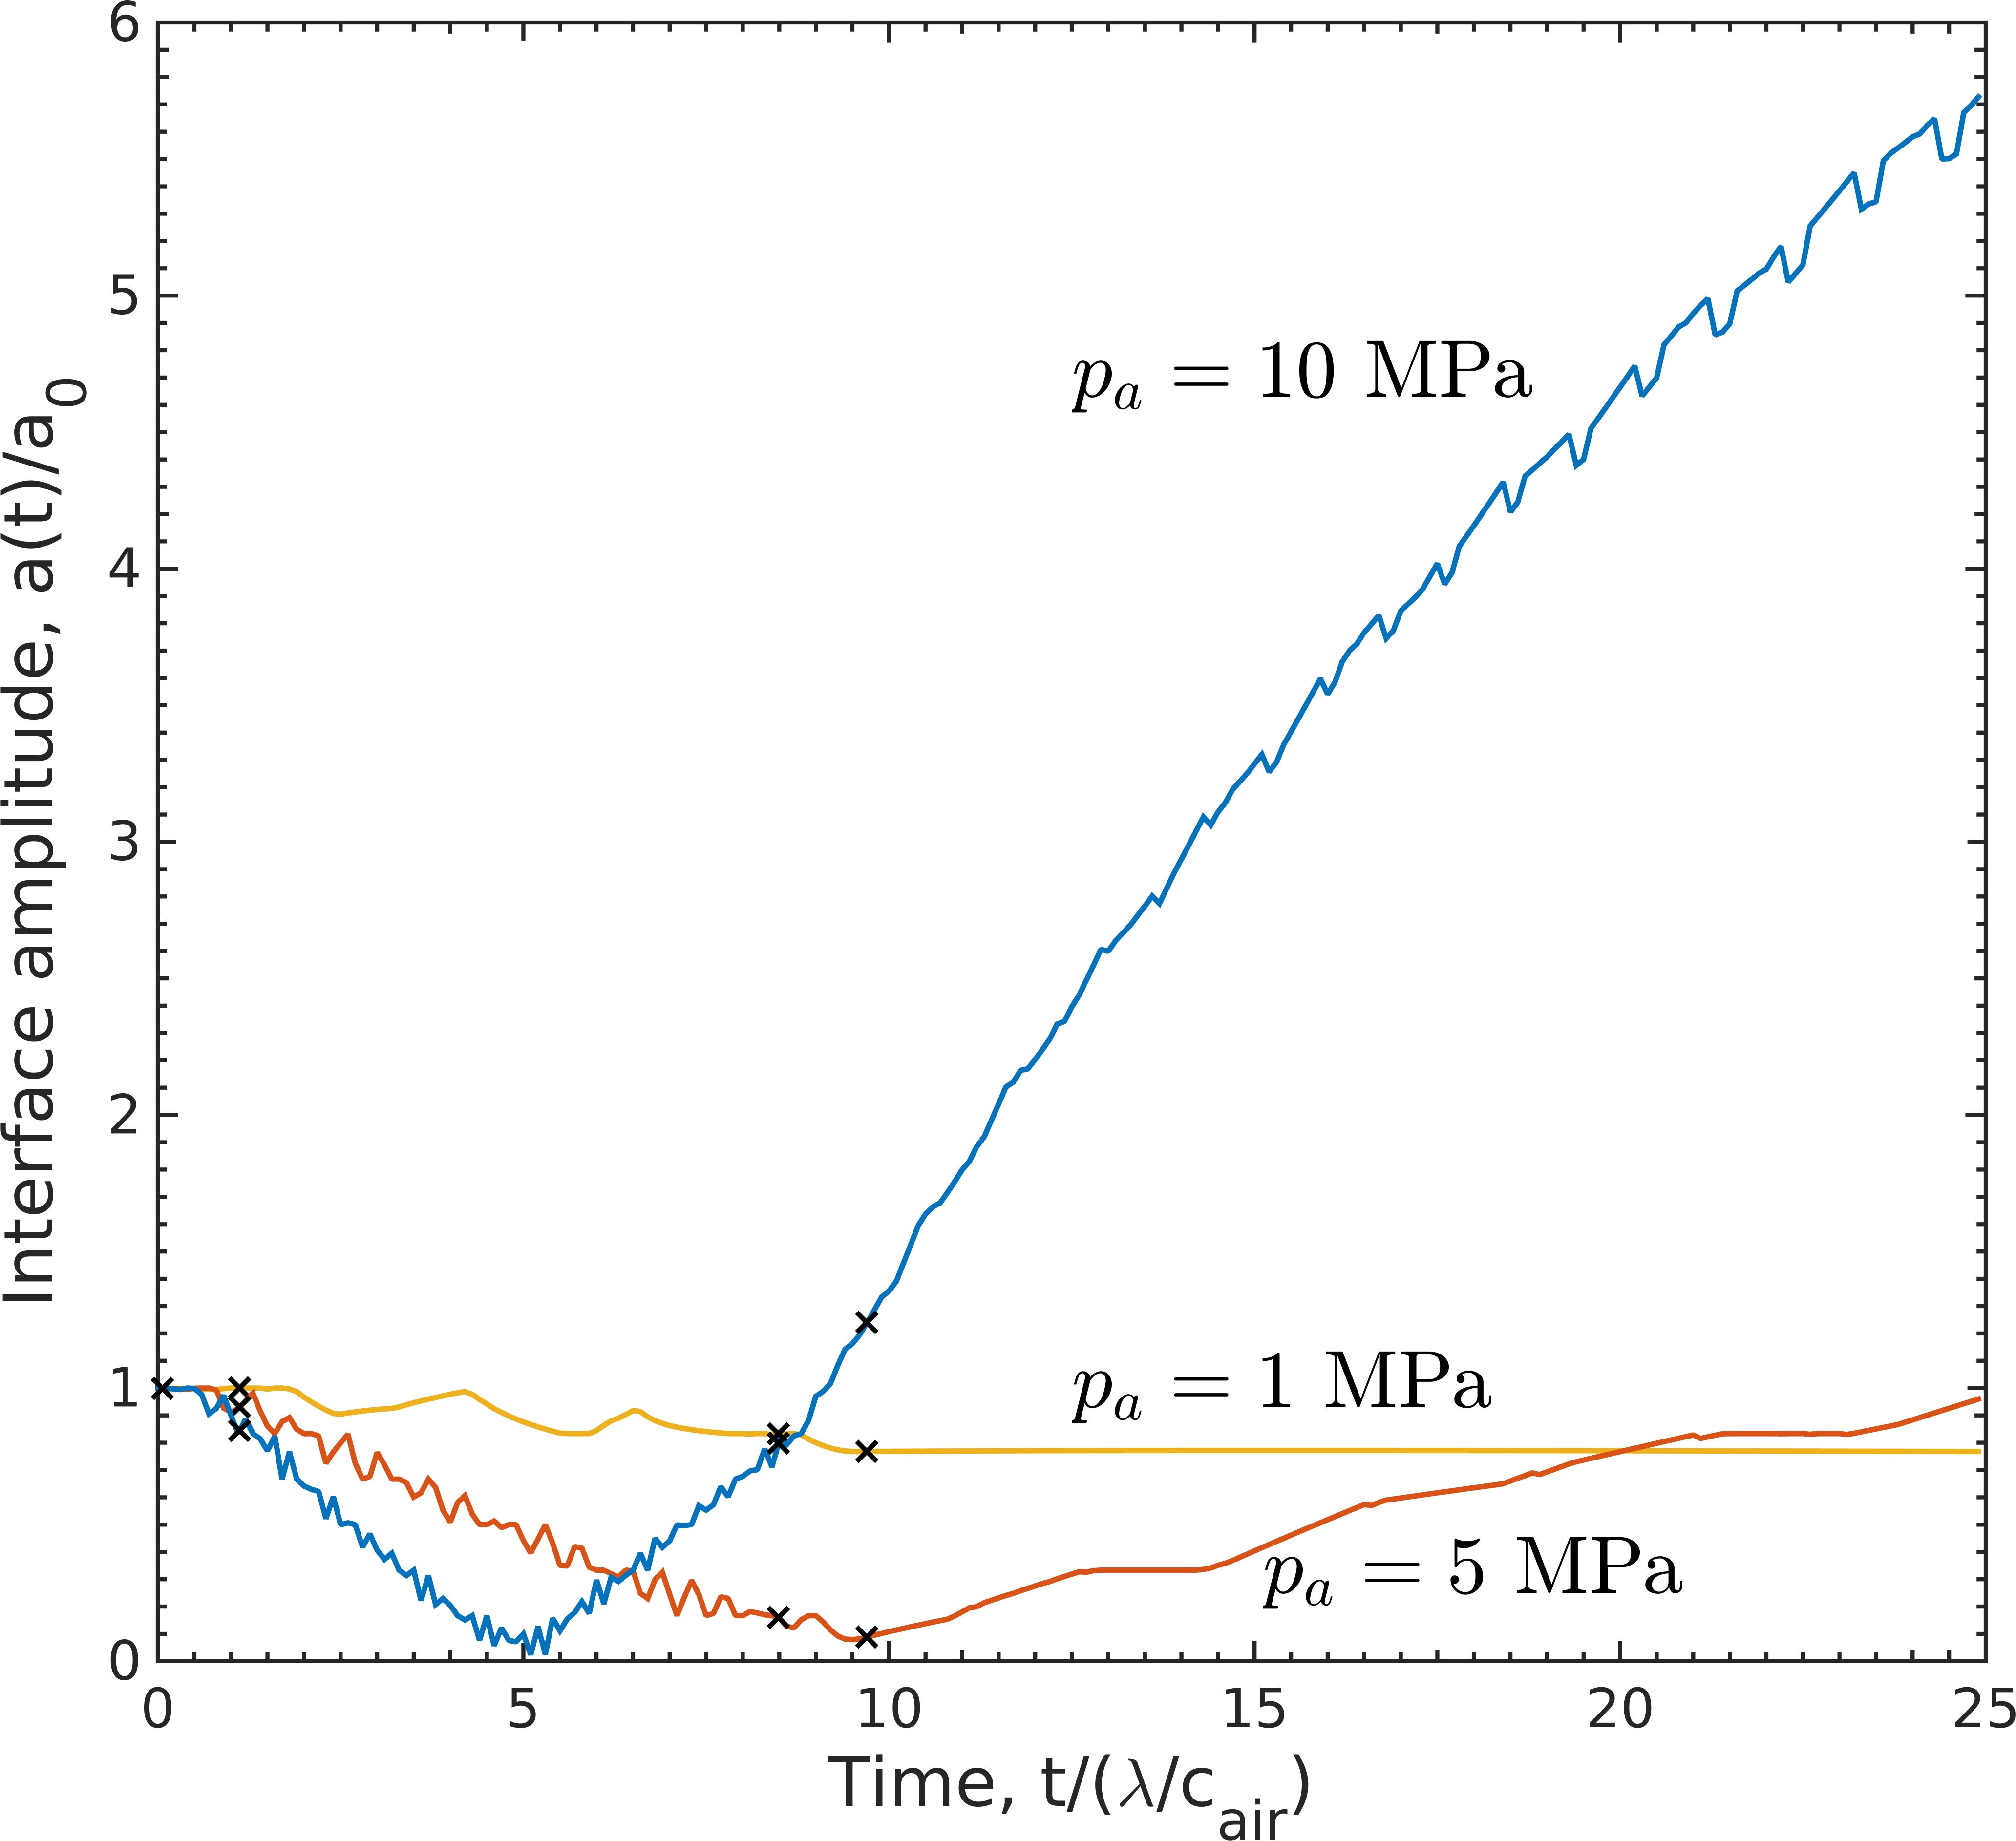
\includegraphics[width=0.48\textwidth]{./figs/lung_figs/interface_multi-amp_norm}
  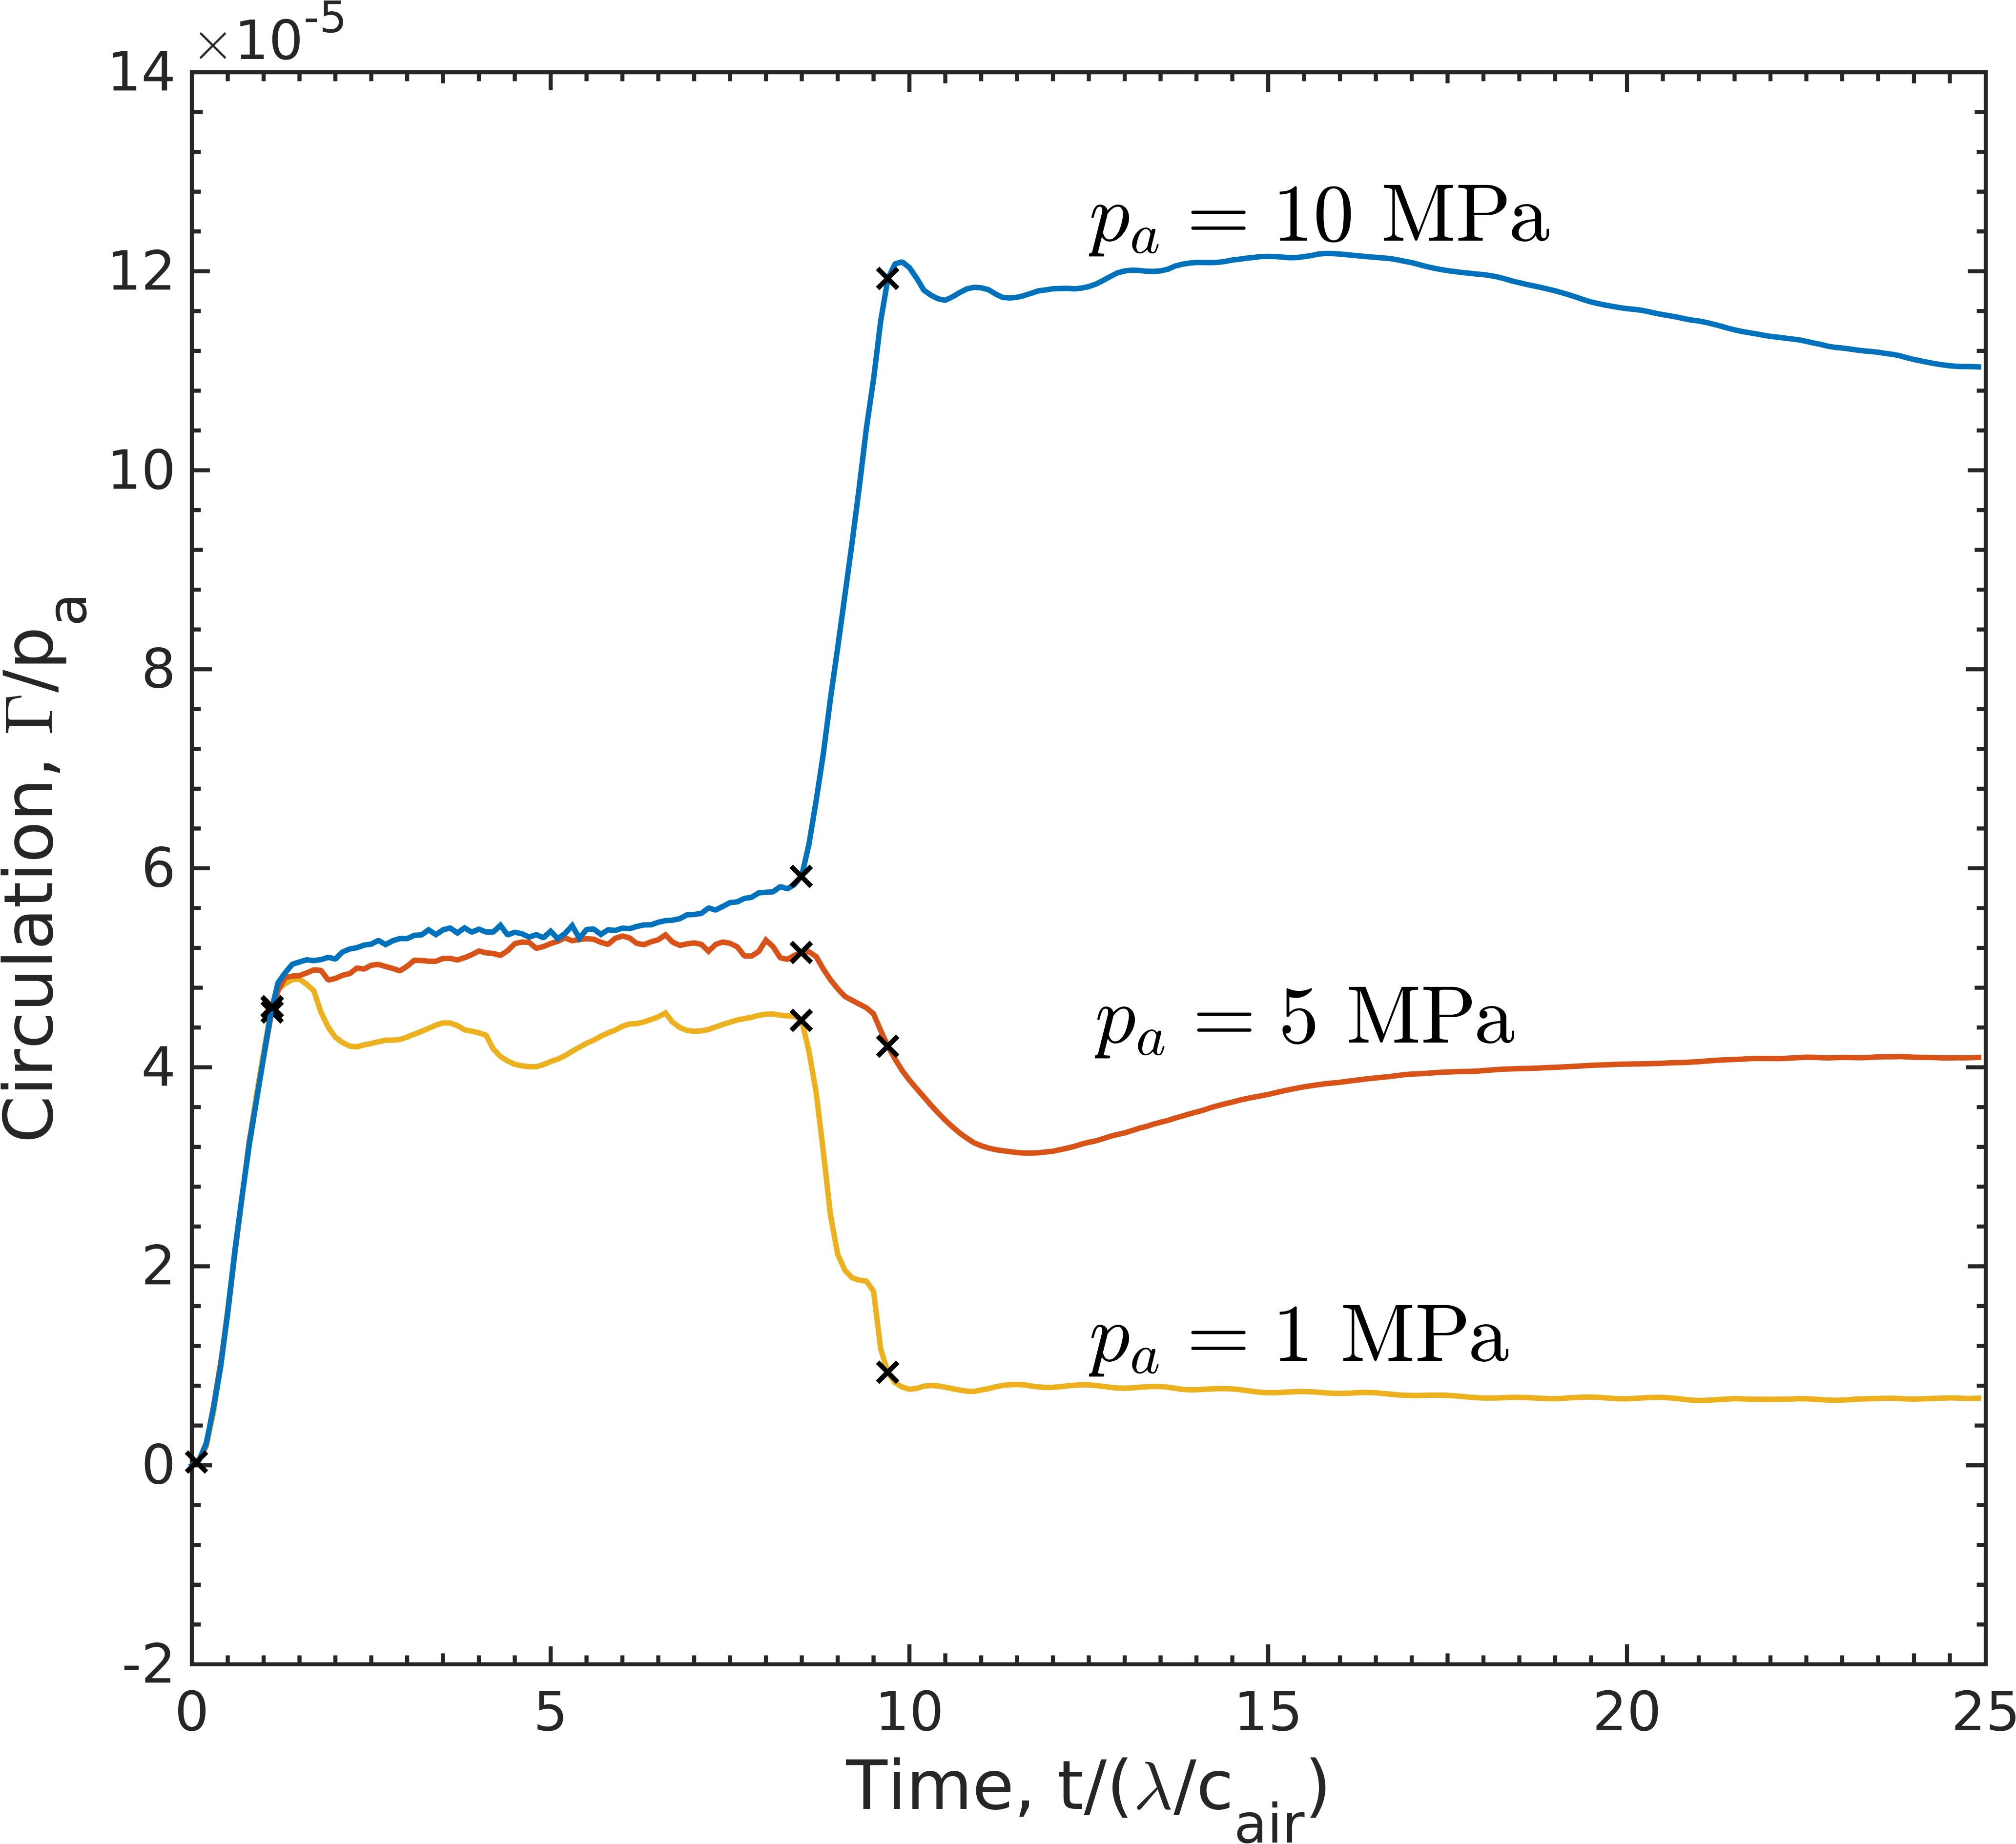
\includegraphics[width=0.48\textwidth]{./figs/lung_figs/circulation_multi-amp_norm}
  \caption[The interface and circulation dependence on wave amplitude at early time]{The interface amplitude (left) and circulation (right)
    histories corresponding to the $1$(yellow), $5$(orange), and
    $10$(blue) MPa trapezoidal waves are shown for $t\leq 25$. The
    circulation history is normalized by the acoustic amplitude of the
    incoming wave to illustrate that circulation deposition by the
    compression wave scales linearly with $p_a$.}
  \label{fig:trapz_circ_interface_early}
\end{figure}
%
\begin{figure}[h] 
  \centering
  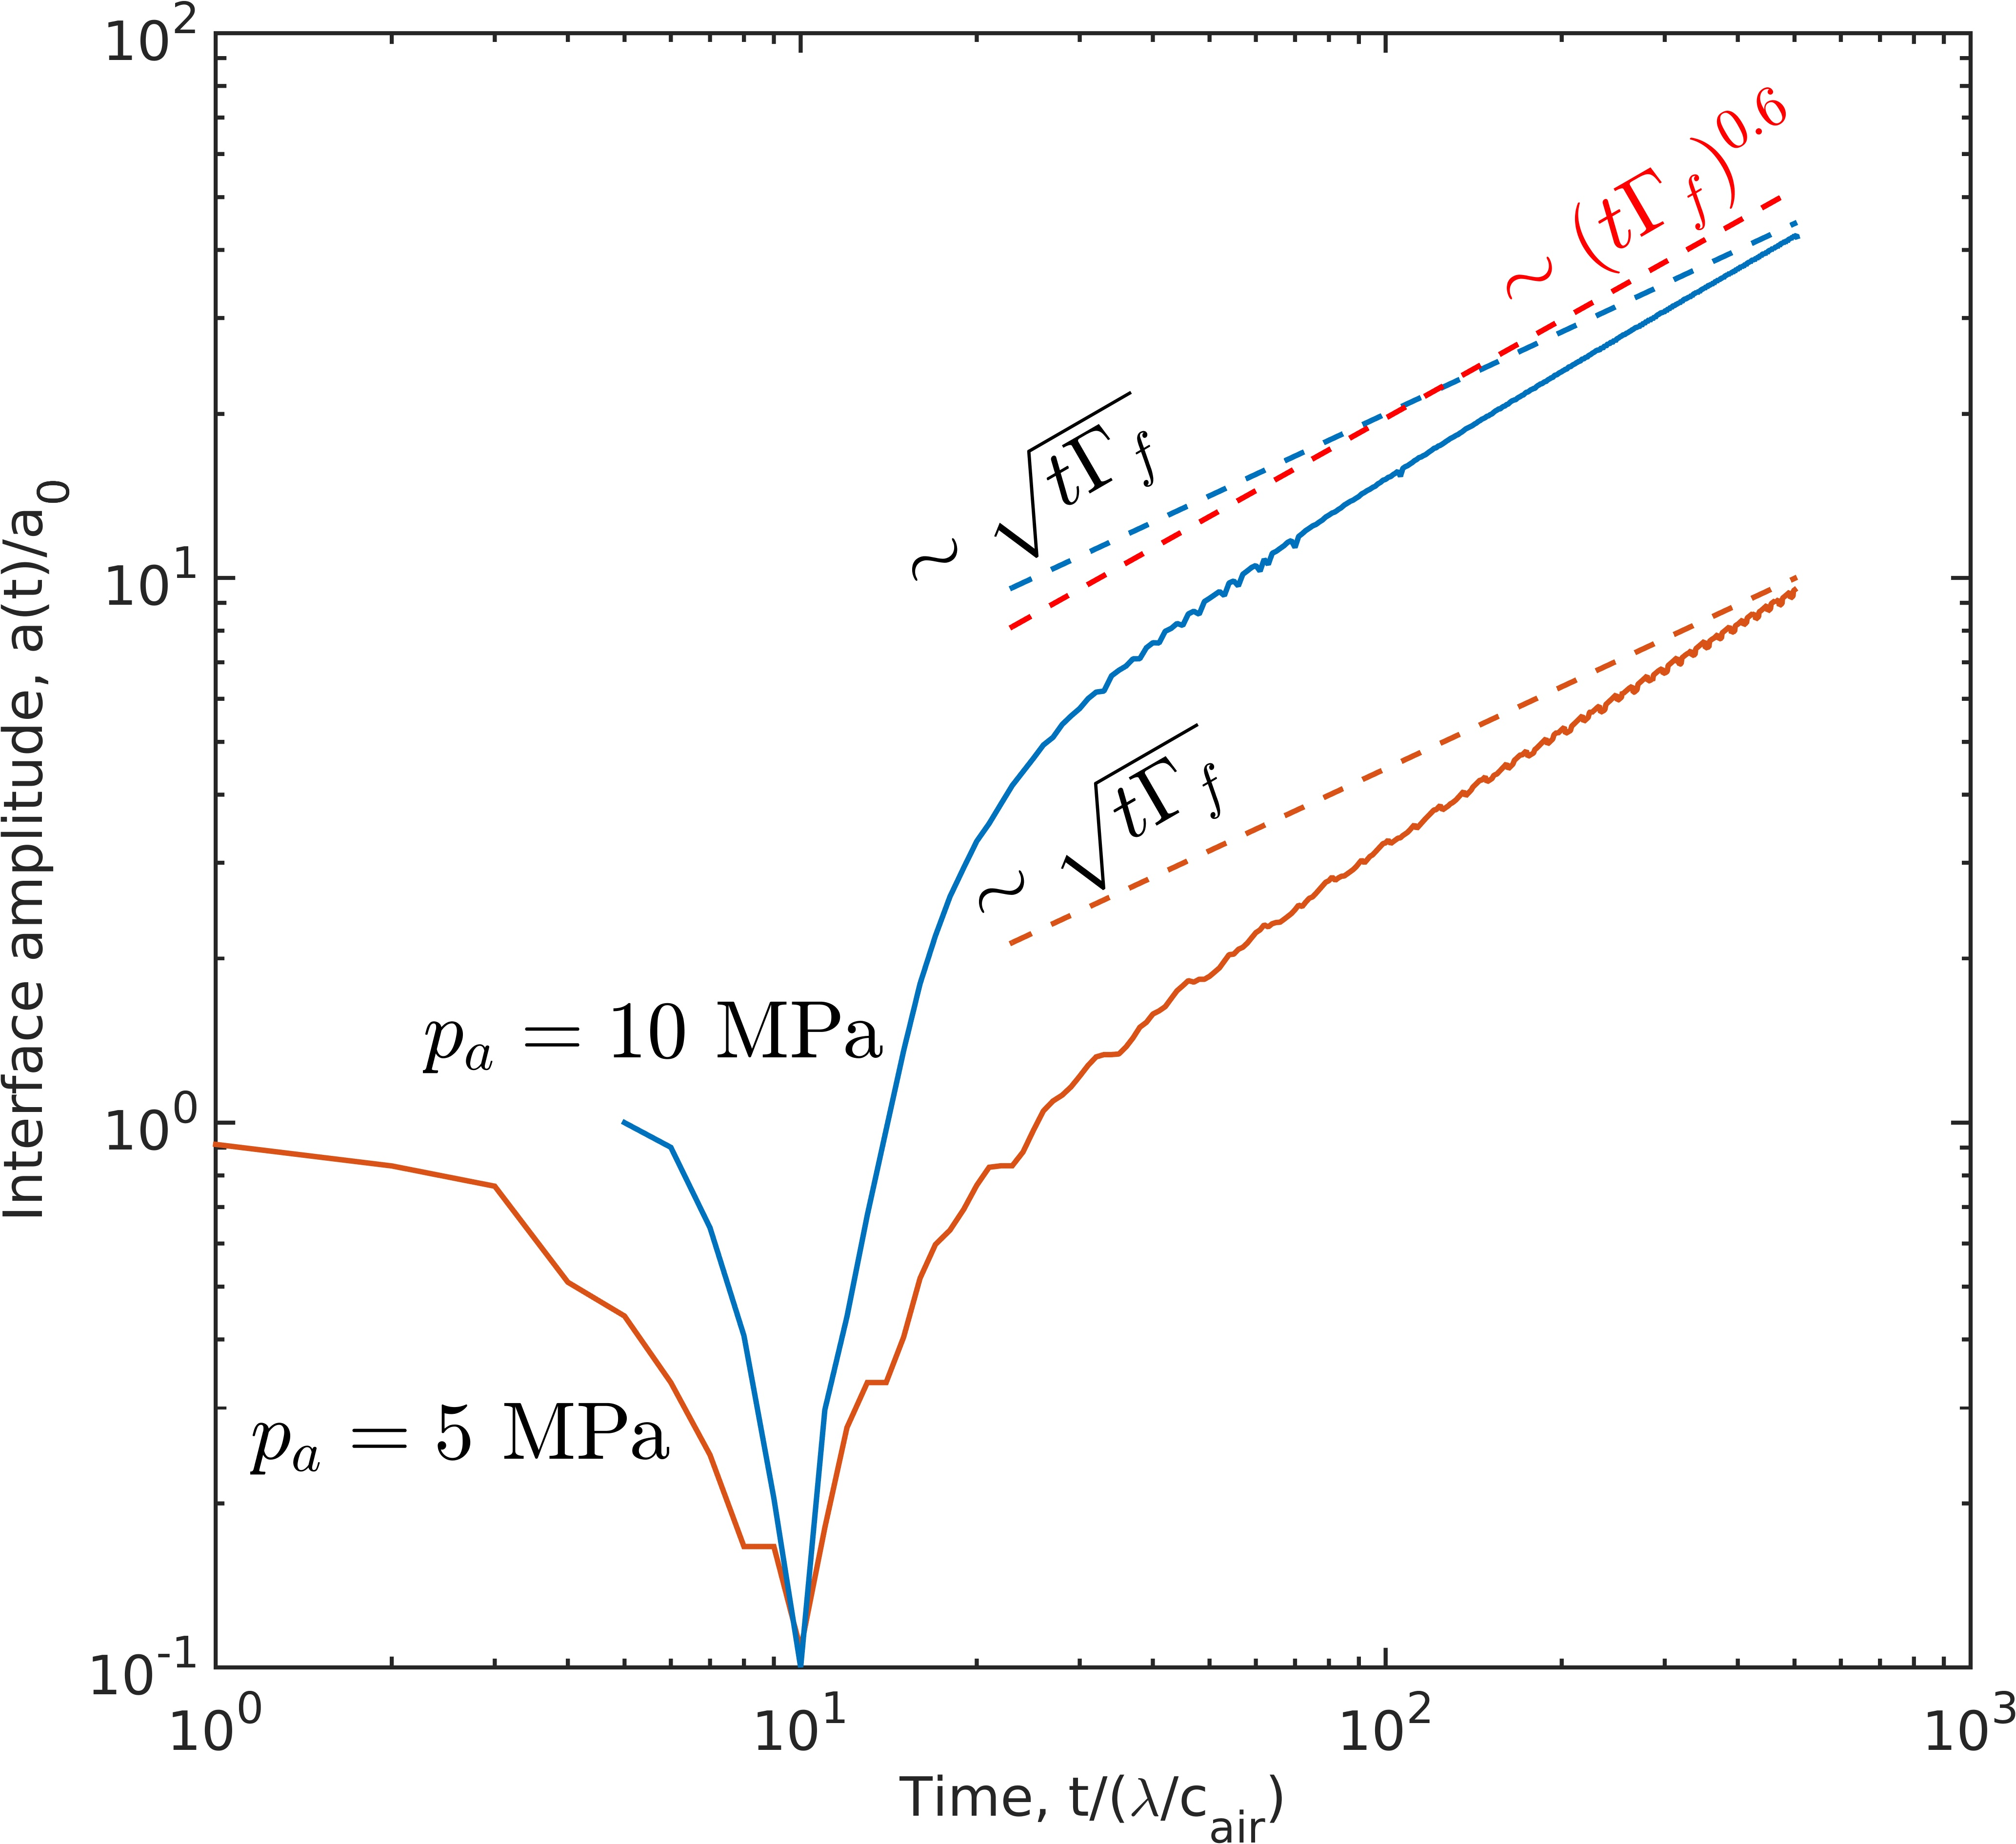
\includegraphics[width=0.48\textwidth]{./figs/lung_figs/interface_multi-amp_loglog_roe_extra}
  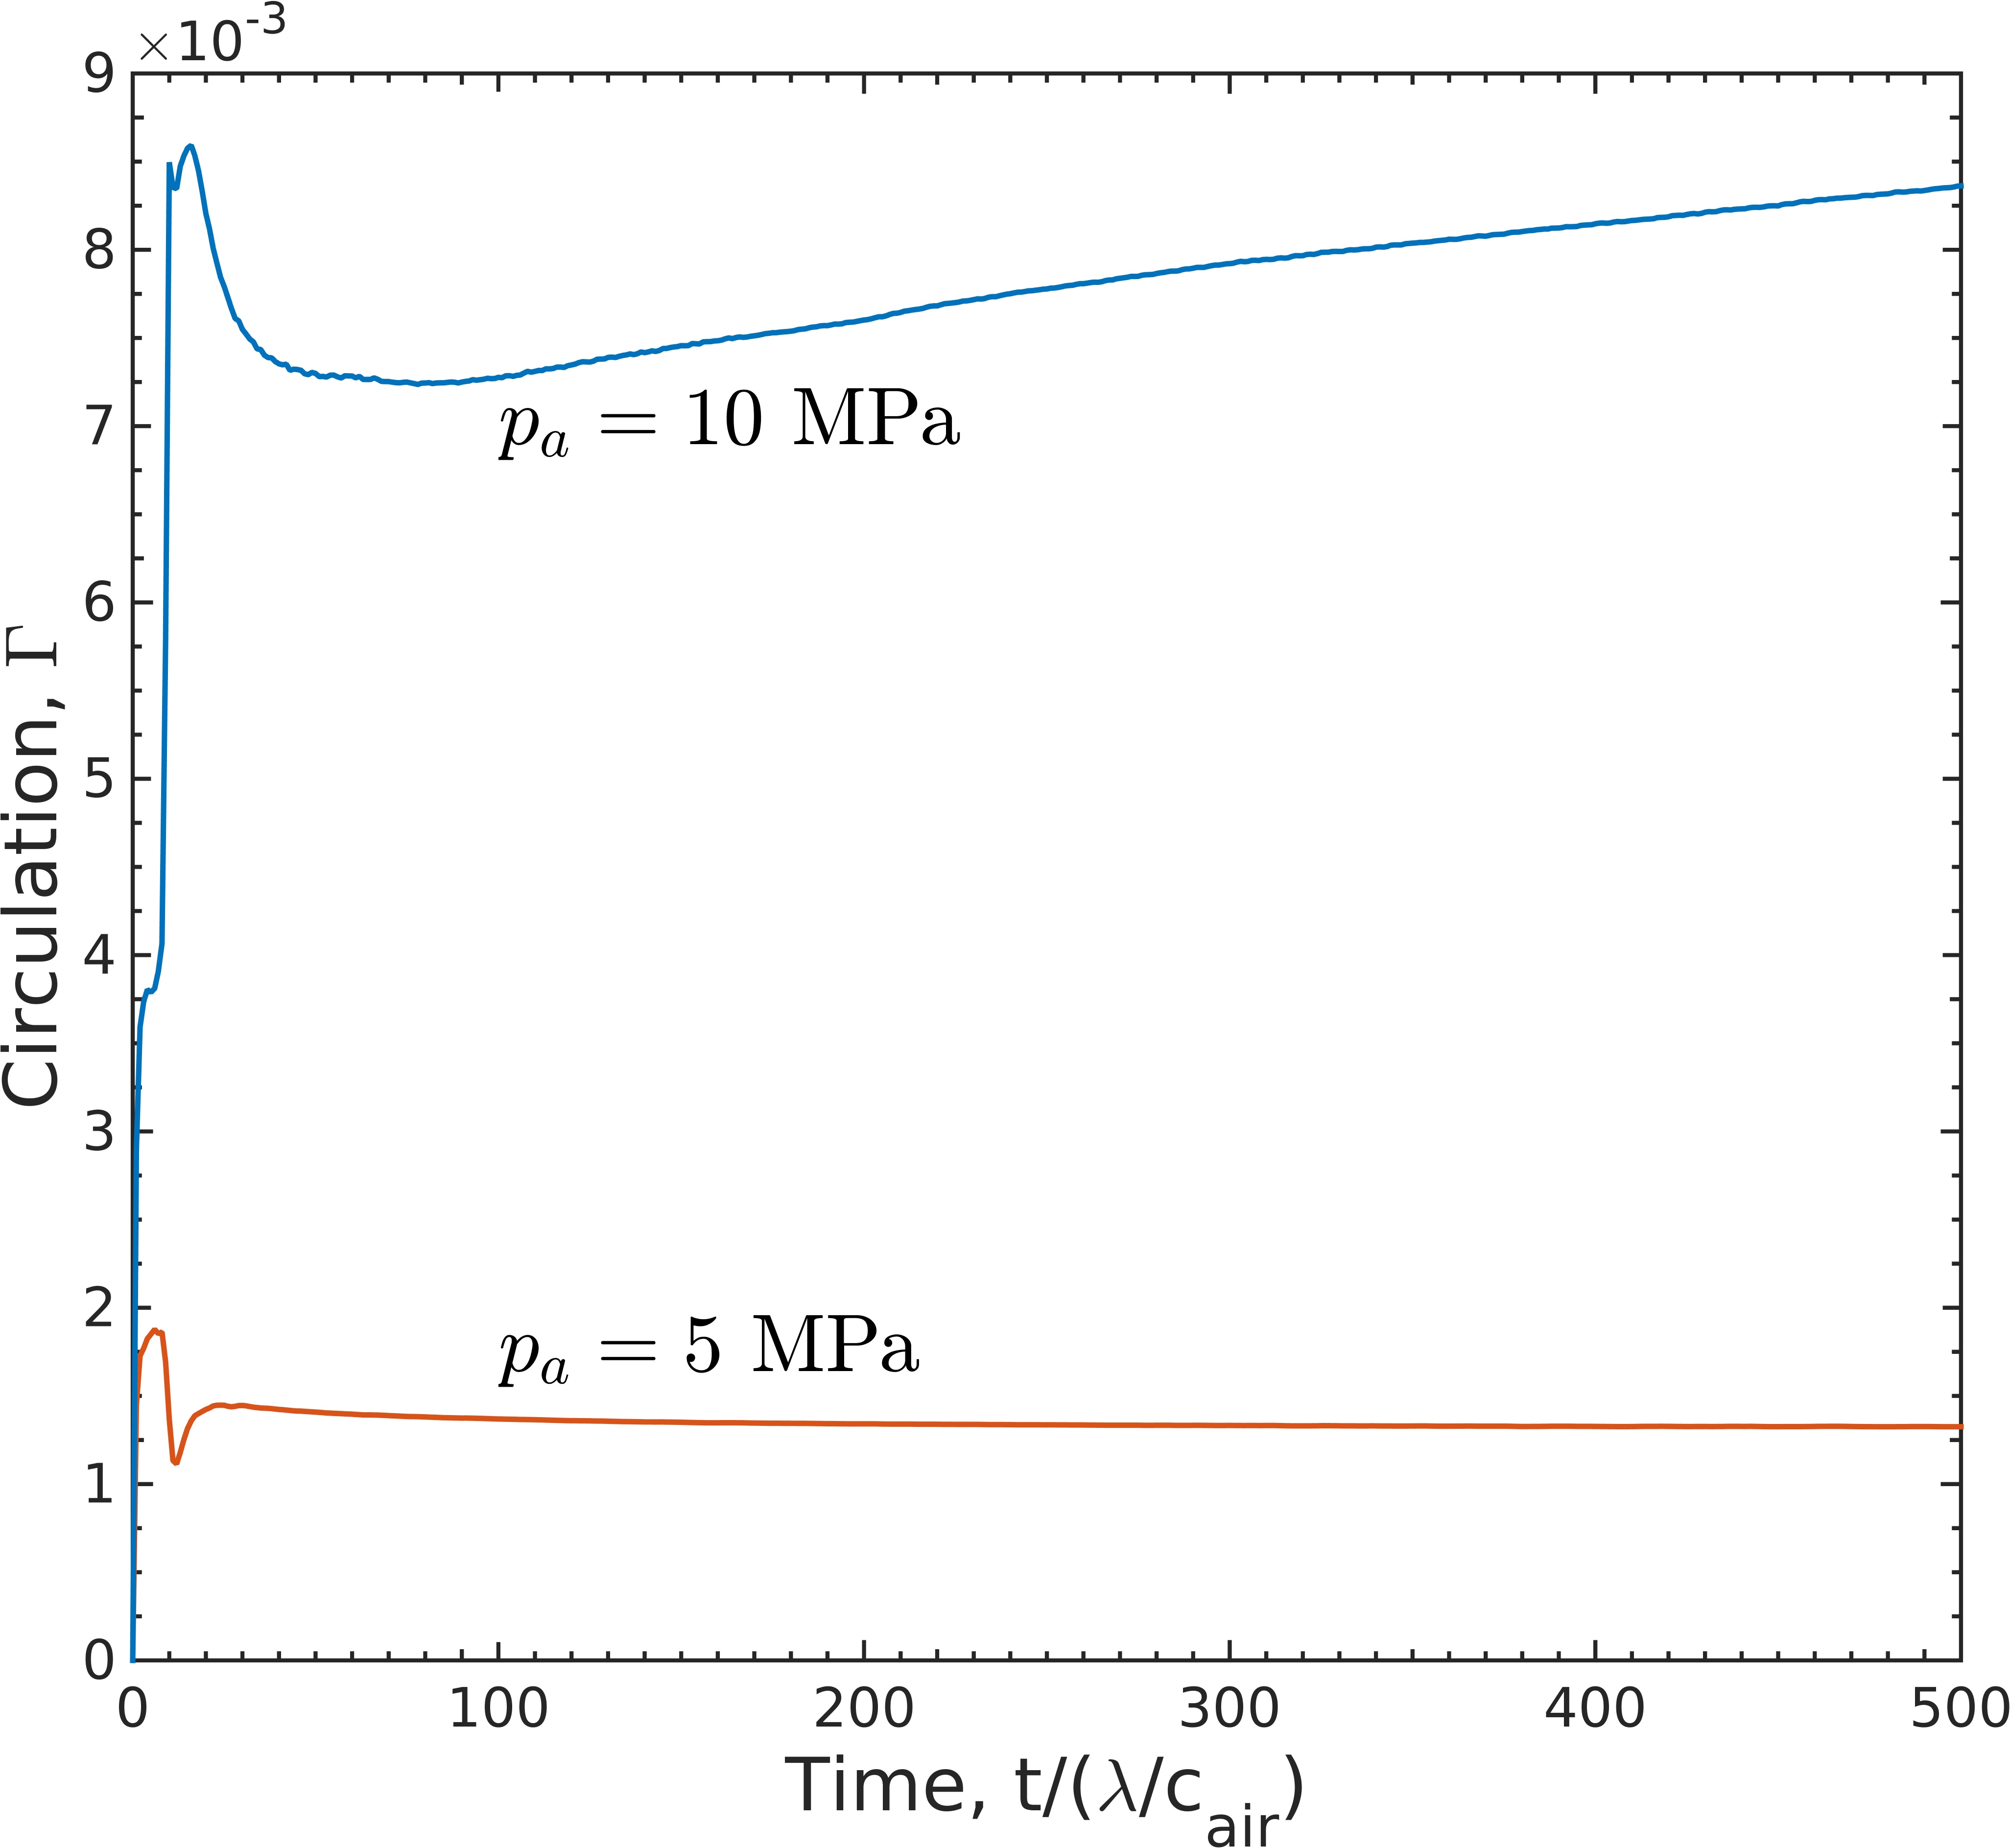
\includegraphics[width=0.48\textwidth]{./figs/lung_figs/circulation_multi-amp2_roe}
  \caption[The interface and circulation dependence on wave amplitude
  at long time]{The interface amplitude (left) and circulation (right)
    histories corresponding to the $5$(orange) and $10$(blue) MPa
    trapezoidal waves are shown for $t\leq 500$. To appropriately
    compare late time dynamics, time has been offset in the interface
    amplitude history such that the phase reversal appears to occur
    simultaneously in both simulations. Dashed lines of the same color
    are used to demonstrate the expected slope of pure circulation
    driven interface growth, based on Equation
    \eqref{eq:intf_circ_scaling}. The red dashed line shows the slope we
    appear to be approaching for the $10$ MPa wave case for the end time.}
  \label{fig:trapz_circ_interface_loglog}
\end{figure}
%
\subsubsection{Dependence on the length of the wave}%
To investigate the dependence of the dynamics on the length of the
trapezoidal wave $L$, and comparably the wave-interface interaction
time, we compare results for $p_a=10$ MPa waves of constant rise and
fall length $\Delta L_a$. This effectively changes the time the
interface has to evolve while experiencing the constant elevated
pressure portion of the wave between the compression and expansion.
Figure \ref{fig:trapz_circ_interface_multi-lag} shows the interface
amplitude and circulation histories corresponding to waves with
$L=45\lambda, 35\lambda ,30\lambda ,25\lambda ,15\lambda ,10\lambda$
for $0 \leq t\leq 25$.  For the three longest waves, $L \geq 30\lambda$,
the expansion encounters the interface after the perturbation reverses
phase. In these cases, the expansion deposits additional positive
circulation along the right half of the interface. For the shorter
waves, $L \leq 25\lambda$, the expansion encounters the interface before
the perturbation reverses phase and the net half-domain circulation is
decreased. Comparing cases in which the interface inverts phase before
the expansion occurs the larger $a(t)$ is at the time, the more
circulation is generated. The same is true when comparing cases in
which the phase inversion occurs after the interface inverts phase.
%
\begin{figure}[h] 
  \centering
  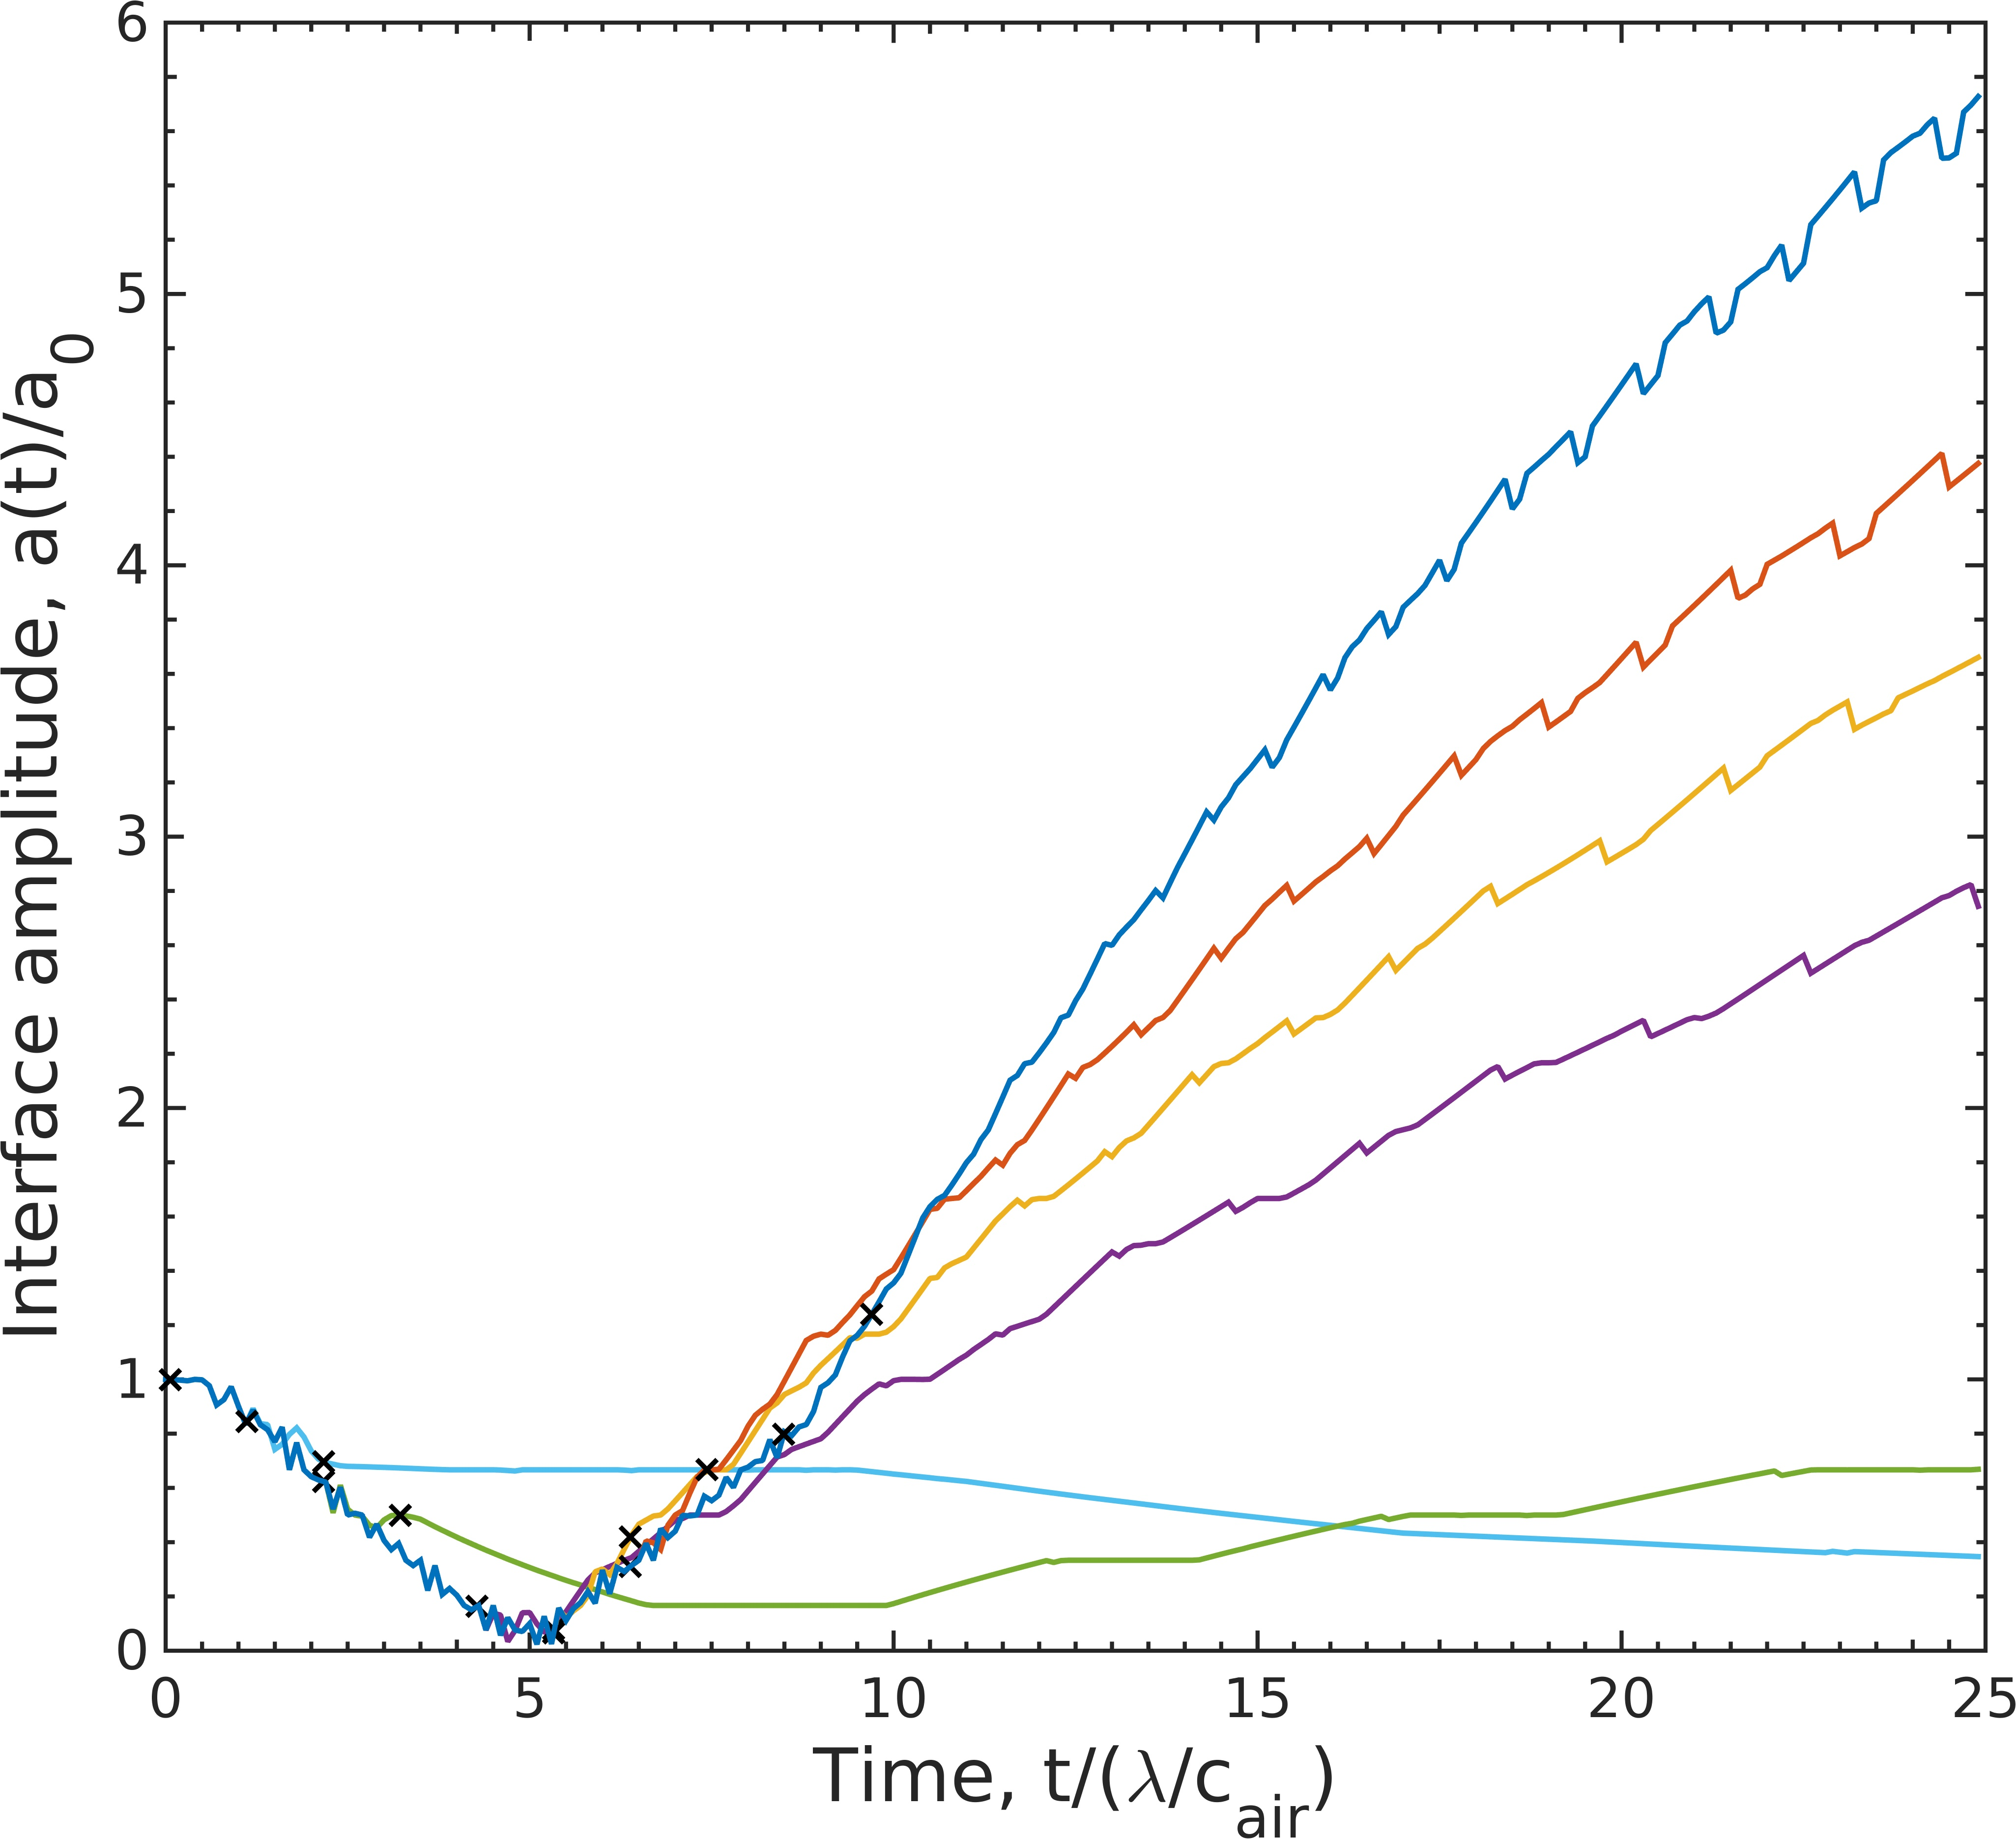
\includegraphics[width=0.48\textwidth]{./figs/lung_figs/interface_multi-lag}
  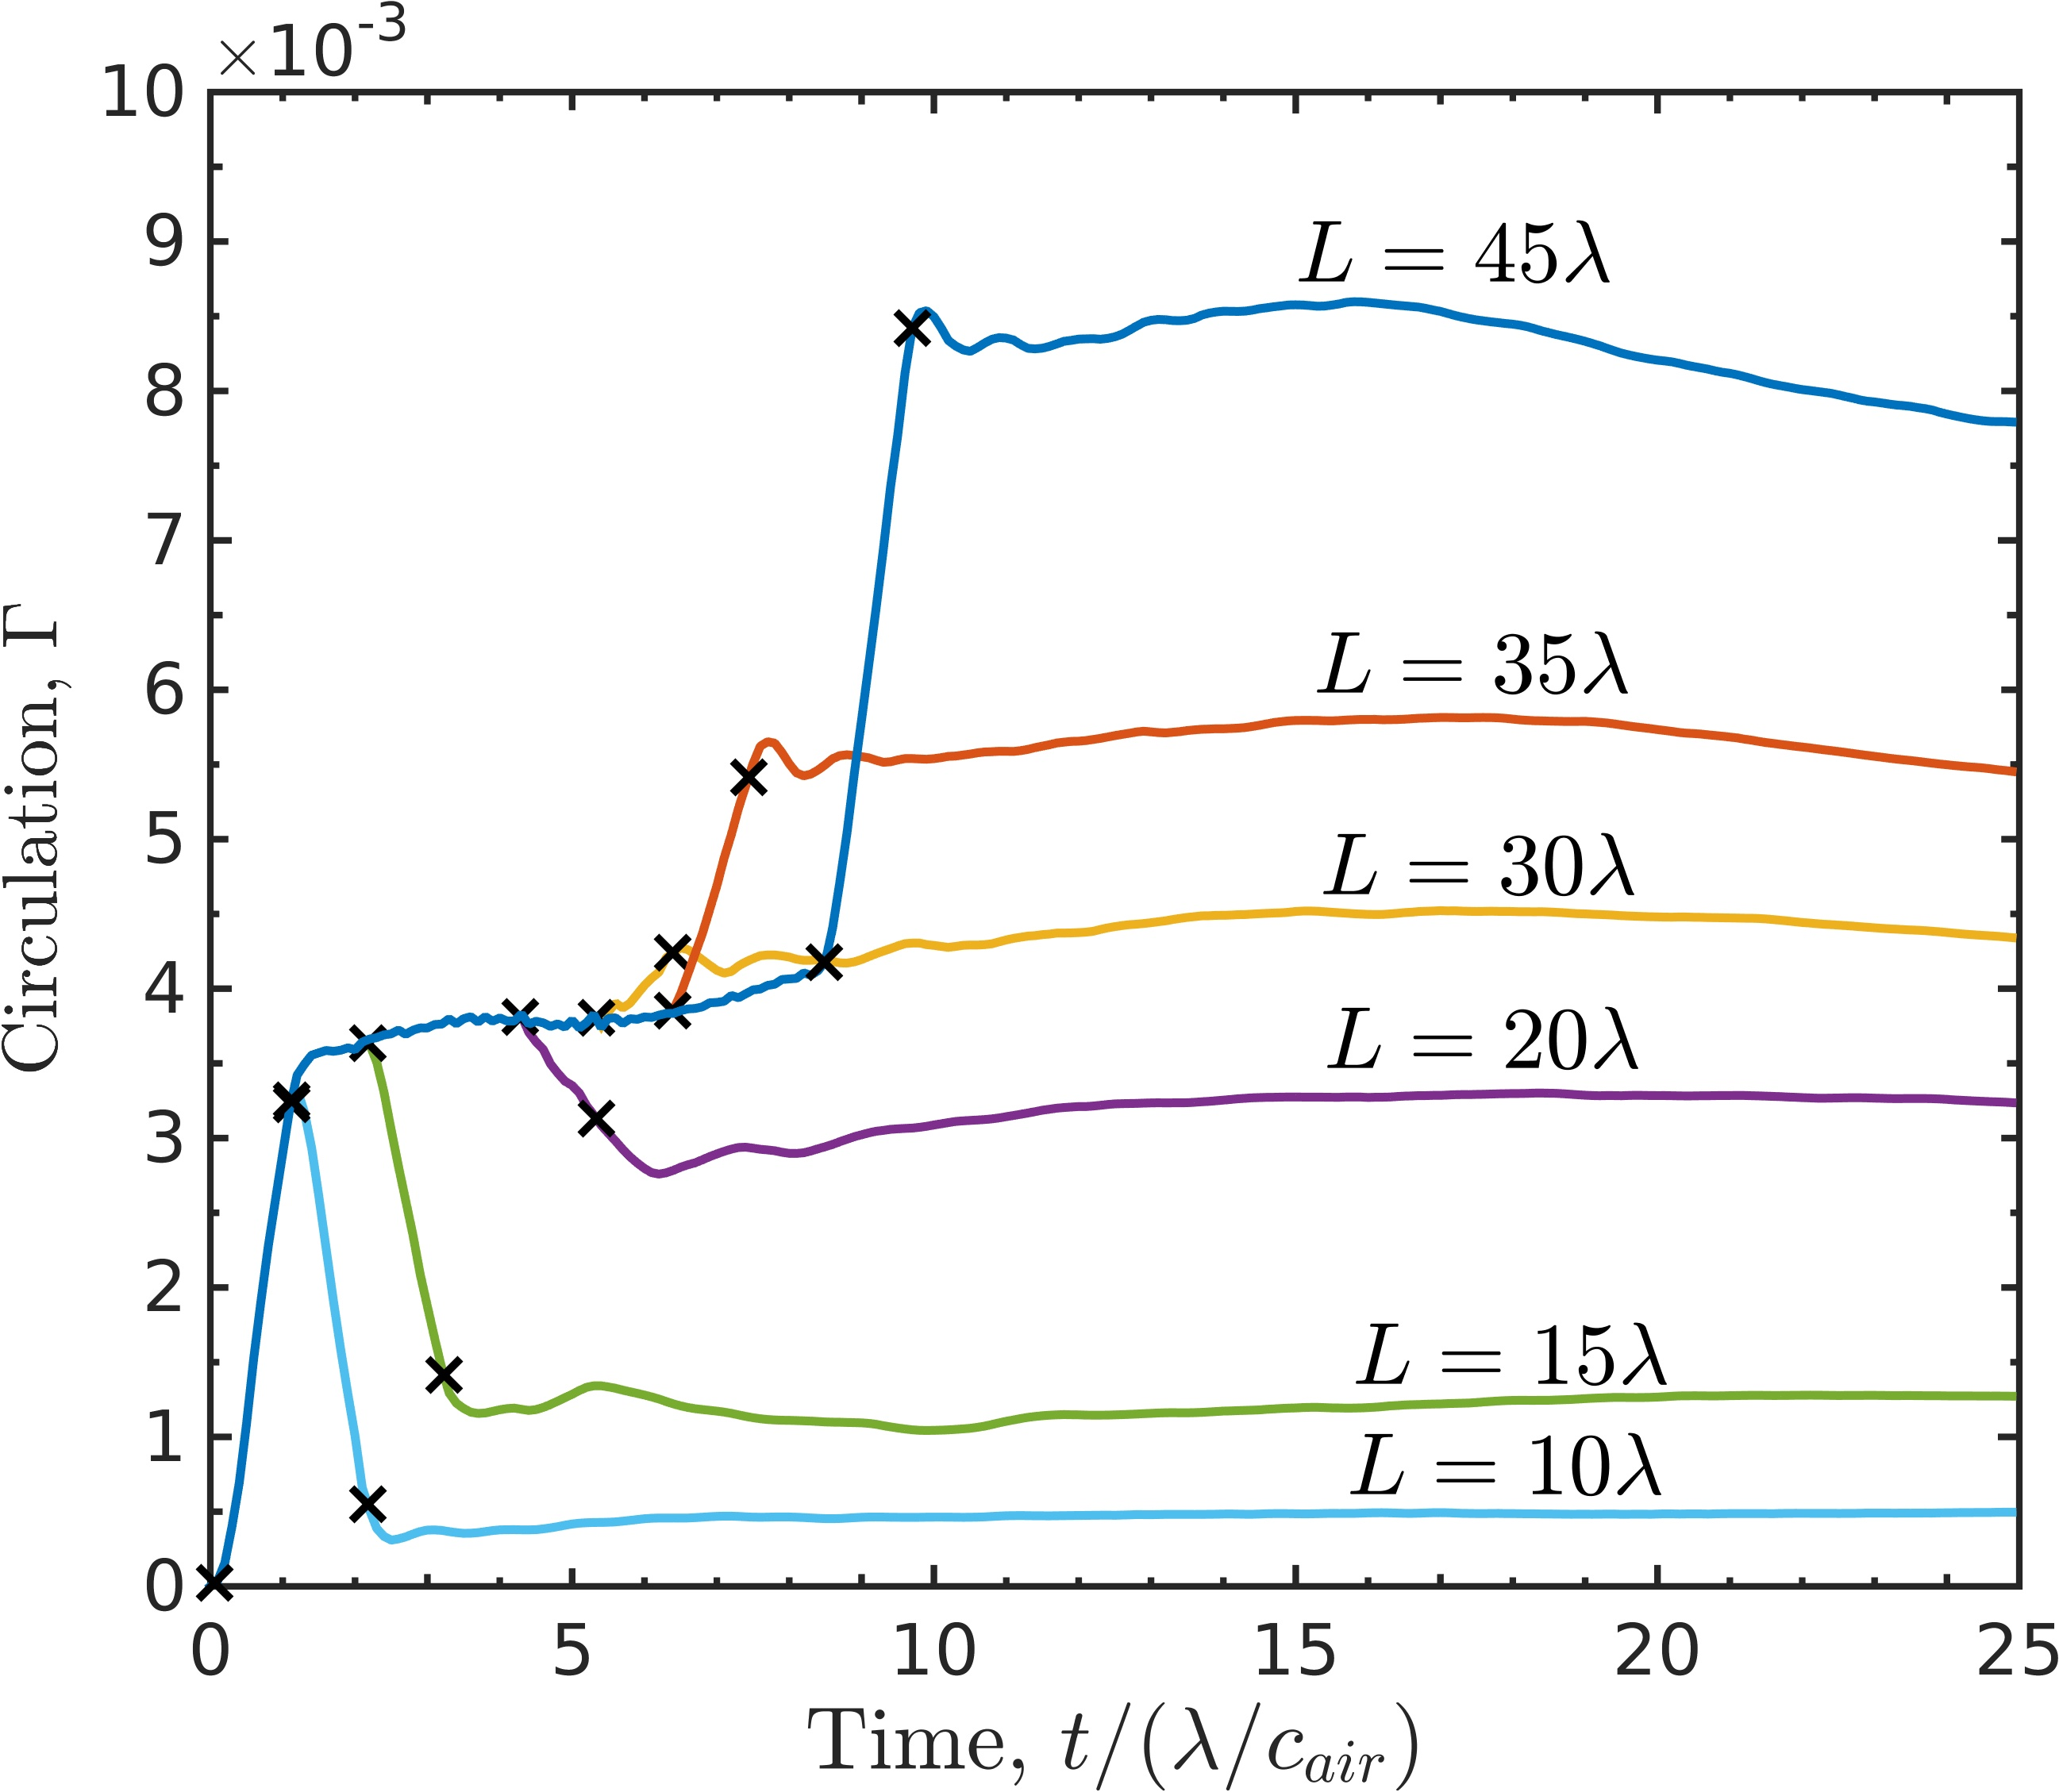
\includegraphics[width=0.48\textwidth]{./figs/lung_figs/circulation_multi-lag_fixed}
  \caption[The interface and circulation dependence on wave
  duration]{The interface amplitude (left) and circulation (right)
    histories for waves of varying total length $L$ and elevated
    static pressure duration between the expansion and compression
    . Here we show results for $L=45\lambda$ (blue), $L=35\lambda$
    (orange), $L=30\lambda$ (yellow), $L=20\lambda$ (purple),
    $L=15\lambda$ (green), $L=10\lambda$ (light blue)}
  \label{fig:trapz_circ_interface_multi-lag}
\end{figure}
%
\subsection{Discussion}
\label{subsec:discussion}
After the passage of the trapezoidal acoustic waves the pressure
returns to the initial, ambient conditions. This implies that the
integral of the pressure gradient $\nabla p$ along the interface, over
all time is zero. Hence we surmise that if the interface remains
unchanged during the interaction with the wave, as it would for a wave
moving with infinite velocity, $\nabla \rho$ would remain constant and
the net baroclinic circulation deposited must be zero. Thus for any
finite duration acoustic wave to deposit net baroclinic circulation
upon an interface, the interface itself must deform during interaction
with the wave. This deformation alters the misalignment of the
pressure and density gradients throughout the passage of the wave such
that vorticity deposited by the compression and expansion waves do not
cancel. Note that this of particular interest for waves in which
the pressure returns to the initial condition after the wave passes,
which is not the case for the traditional shock-accelerated \ac{RMI}
problem.

For the cases varying the length of the wave $L$, we previously noted
that whether the expansion increased or decreased the total
half-domain circulation depended on whether it encountered the
interface before or after the phase change. If indeed circulation is
driving the deformation of the interface, then changes in the waveform
that appear to have very little effect on the interface dynamics
during the wave-interface interaction period, may have far more
significant impacts on the long term dynamics of the interface via
vorticity.

%% Local Variables:
%%% mode: latex
%%% TeX-master: "../main"
%%% End:


%\section{Analysis}%
\label{sec:analysis}%
We perform analysis to make quantifiable predictions about the
vorticity generation and interface growth. The results of these
analyses are compared with the results of our numerical experiments in
section \ref{sec:results}.

To better understand the source of circulation within our problem we
look to the vorticity generation equation for a 2D inviscid fluid
system,
\begin{align} \label{eq:vorticity_euler}
  \frac{\partial \vec{\omega}}{\partial t}+\left(\vec{u}\cdot\nabla\right)\vec{\omega} =% 
  - \vec{\omega}\left(\nabla\cdot\vec{u}\right) + \frac{\nabla\rho\times\nabla p}{\rho^2}.%
\end{align}
Each term in equation \eqref{eq:vorticity_euler} represents a
different physical mechanism by which the vorticity $\vec{\omega}$ is
changing, with the terms on the left-hand side represent changes in
the existing vorticity field and the terms on the right representing
vorticity sources and sinks. The first term on the left represents the
total change of vorticity at a location in the flow field with respect
to time. The second term on the left represents the advection of
vorticity within the field. The first term on the right describes
changes in vorticity due to compressibility in the flow. The last term
on the right is the baroclinic term which describes vorticity
generated by the misalignment of the pressure and density gradients in
the flow. We seek to understand the relative importance of these
mechanisms on the dynamics of the acoustically accelerated interface.

\subsection{Order of magnitude analysis of vorticity generation mechanisms}
To quantifiably compare the various mechanisms by which vorticity
changes within the flow, we recognize that any vorticity generated
must be a result of acoustic energy being converted to kinetic energy
within the flow. As the only mechanism for this to occur in an
inviscid fluid without pre-existing vorticity is baroclinic, we
require misaligned density and pressure gradients. Thus we choose to
perform our analysis at the water-air interface during the period
which is interacting with the incoming wave. For simplicity, we narrow
this down even further to only consider the period in which the
incoming compressive portion of the wave encounters the interface. As
this interaction occurs quickly, over an approximate time span
$\Delta t_a\approx5\lambda/c_{w}$, we assume that the interface is
static and remains undeformed from its initial state during this
interaction. We will show in section \ref{sec:results}, this is a
reasonable assumption for this period. Having now established the
point at which the analysis is to be performed we evaluate the order
of magnitude of compressible, advective, and baroclinic terms of the
vorticity generation equation \eqref{eq:vorticity_euler}. We note that
the advective term is not a true source of vorticity, but is useful in
understanding the change of vorticity at any given time and location
within the flow.

In our evaluation of the individual terms of the vorticity generation
equation \eqref{eq:vorticity_euler}, we treat gradient, curl, and
divergence terms of any arbitrary quantity $f$ such that
$\nabla f= \orderof{\left|\Delta f\right|/\Delta L}$,
$\nabla\cdot f=\orderof{\left|\Delta f\right|/\Delta L}$, and
$\nabla\times f=\orderof{\left|\Delta f\right|/\Delta L}$. Here
$\Delta f$ is a change in $f$ over a characteristic length scale
$\Delta L$. Because the only motion in the flow is generated by the
acoustic wave. Accordingly, we consider acoustic pressure, velocity,
and density perturbations such that $\Delta p=\Delta p_a$,
$\Delta \vec{u}=\Delta \vec{u}_a$, and $\Delta \rho=\Delta \rho_a$,
and use acoustic relations to relate these quantities
\citep{Anderson1990},
\begin{align}%
  \label{eq:acoustic_relations}%
  \Delta p_a=\pm\Delta u_a \rho c=c^2\Delta \rho_a%
\end{align}
Additionally, for the values presented in this section we consider our base
trapezoidal wave case where $p_a = \Delta p_a = 10$ MPa. The length
scale associated with the acoustic wave is the initial length of the
pressure rise $\Delta L_a=5\lambda$. The initial interface length
scale $\Delta L_I$, defined as the thickness of the thickness of the
mixed layer from 0.05 to 0.95 volume fraction is estimated as
$\Delta L_I \approx 0.05\lambda$. We approximate the order of theta
based on its average value along a half-wavelength of the interface
for $a_0=0.03\lambda$ such that $\overline{\abs{\theta}}\approx0.12$.

To assess the baroclinic contribution to vorticity, we write the cross
product of the density and pressure gradients as
$\abs{\nabla \rho} \abs{\nabla p} \sin{\left(\theta\right)}$. Here
$\theta$ is the angle between the acoustic pressure gradient, treated
as being in the $\plus y$-direction, and the direction of the density
gradient which we treat as the outward normal direction to the
interface. For $a_0/\lambda<<1$, we can approximate
$\sin{\left(\theta\right)}\approx\theta$ at the interface. The density
gradient due to the water-air interface is far greater than that due
to the acoustic wave. As such we use the change in density across the
interface $\Delta \rho_I$ and associated length scale $\Delta L_I$ to
write the density gradient. The pressure change is a result of the
acoustic wave, and as such we use the acoustic pressure change
$\Delta p_a$ and associated length scale $\Delta L_a$ to express the
pressure gradient. And thus we write the order of magnitude of the
baroclinic vorticity generation term at the interface,
\begin{align}
  \label{eq:baroclinic_vorticity}%
  \norm{\frac{\nabla\rho\times\nabla p}{\rho^2}} = \orderof{\frac{\abs{\Delta \rho_I}}{\abs{\Delta L_I}}\frac{\abs{\Delta p_a}}{\abs{\Delta L_a}}\frac{1}{\abs{\rho}^2}\abs{\theta}}.%
\end{align}

In the evaluation of the compressible and advective terms we consider
two possible evaluations of the vorticity $\omega$ as either the curl
of the acoustic velocity field $\vec{\omega}=\nabla\times\vec{u}$ or
the integral of the baroclinic vorticity generation term from
\eqref{eq:baroclinic_vorticity}, treated as constant, over the
characteristic time of the pressure rise
$\Delta t_a\approx\Delta L_a/c_w$. Evaluating the vorticity using both
of these expressions and the previously presented values reveals that
the baroclinic expression of the vorticity is dominant for
the regimes of interest to this study and is thus what we will focus
on in our further analysis. Hence we write an expression for the
approximate order of magnitude of the compressible and advective
contribution to vorticity as
\begin{align}
  \label{eq:compressible_advective_vorticity}%
\norm{-\vec{\omega}\left(\nabla\cdot\vec{u}\right)}\sim \norm{\left(\vec{u}\cdot\nabla\right)\vec{\omega}} = %
\orderof{\frac{\abs{\Delta u_a}}{\abs{\Delta L_a}} \frac{\abs{\Delta \rho_I}}{\abs{\Delta L_I}}\frac{\abs{\Delta p_a}}{\abs{\Delta L_a}}\frac{1}{\abs{\rho}^2}\abs{\theta}\frac{\abs{c}}{\abs{\Delta L_a}}}.%
\end{align}

Now, to compare the relative importance of the baroclinic and
compressible (or advective) contributions to vorticity we will look at
the ratio of the two vorticity generation approximations. We divide
equation \eqref{eq:baroclinic_vorticity} by equation
\eqref{eq:compressible_advective_vorticity} use
\eqref{eq:acoustic_relations} to express acoustic quantities in terms
of the acoustic perturbation quantities $\Delta \rho_a,\,\Delta u_a$ and simplify,
\begin{align} \label{eq:vorticity_comparison}
\frac{\norm{\frac{\nabla\rho\times\nabla p}{\rho^2}}}{\norm{-\vec{\omega}\left(\nabla\cdot\vec{u}\right)}} = \frac{c}{\abs{\Delta u_a}} = \frac{\rho}{\abs{\Delta \rho_a}}%
\end{align}
Evaluating this expression we expect that the relative contribution of
baroclinic to compressible/advective vorticity generation is
approximately of order $\orderof{10^2}$ at
$t=\Delta t_a=1.05$. Hence we expect that the total circulation within
the left and right halves of domain to be nearly entirely
baroclinically generated, and thus we will neglect vorticity generated
through other mechanisms as we continue with our analysis.

\subsection{Comparison of vorticity generation in air and water}
Having established that the dominant source of vorticity is
baroclinicity we now aim to determine where this vorticity will
generated within the mixed region of the interface. Specifically, we
aim to compare the order of baroclinic vorticity generation from
equation \eqref{eq:baroclinic_vorticity} in pure water and air. As
this can already be evaluated in water from what we have provided up
to this point, we will focus on evaluation of the order of baroclinic
vorticity generation in air, from equation
\eqref{eq:baroclinic_vorticity}. Throughout the analysis we will
denote the properties of the incoming wave and water with a subscript
$-$, and the transmitted wave and air with a subscript $+$. For water,
we will use the values for
$\Delta \rho_I, \Delta L_I, \Delta \rho_a, \Delta L_a$ and $\theta$
defined in the previous section based on our initial condition. Our
treatment of the density gradient at the interface will remain
unchanged for evaluation in air such that
$\Delta \rho_I^-=\Delta \rho_I^+$ and $\Delta L_I^-=\Delta L_I^+$.

To evaluate the remaining terms in air we will borrow techniques from
linear acoustics. To find the pressure change in the transmitted wave
$\Delta p_a^+$, we recognize that $a_0/\lambda<<1$ and treat the
incoming wave as a plane wave impinging normally on a flat material
interface such that $\Delta p_a^+=\bs{T} \Delta p_a^-$, where $\bs{T}$
is the acoustic transmission coefficient,
$\bs{T}=2\rho^+ c^+/\left(\rho^+ c^+ + \rho^- c^- \right)$
\citep{Kinsler1982}. For our water-air interface
$\bs{T}\approx4.97\times10^{-4}$. Because of the strong impedance
mismatch between fluids, the acoustic wave is almost entirely
reflected, decreasing the pressure gradient in the air. Because of the
drop in sound speed across the interface, the transmitted wave is
compressed into a smaller physical area (i.e., the wavelength
decreases) relative to the incoming wave, such that
$\Delta L_a^+=\Delta L_a^- (c^+/c^-)$. This effect increases the
pressure gradient in the air. To evaluate $\theta^+$, we utilize
Snell's law which states that
$c^-\sin{\theta^-}=c^+\sin{\theta^+}$. Because $a_0/\lambda<<1$ it is
also true that $\theta^-<<1$, thus we use the small angle
approximation of $\sin$ to find that
$\theta^+\approx\theta^-(c^+/c^-)$. We note that this decreases the
misalignment between the pressure and density gradients in air, and
quantitatively approximately cancels the increase in pressure gradient
due to the decrease in wavelength of the transmitted wave.

To determine where the vorticity will be generated at the interface,
we consider equation \eqref{eq:baroclinic_vorticity} in air and water
and write the ratio to find
\begin{align}%
\label{eq:baroclinic_air_water}%
%\left(\frac{\partial\omega}{\partial t}\right)_{\substack{\text{baroclinic}\\\text{air}}} / \left(\frac{\partial\omega}{\partial t}\right)_{\substack{\text{baroclinic}\\\text{water}}}%
\frac{\norm{\frac{\nabla\rho\times\nabla p}{\rho^2}}_{air\quad}}{\norm{\frac{\nabla\rho\times\nabla p}{\rho^2}}_{water}}
=&\orderof{\frac{\left[\frac{\abs{\Delta \rho_I^+}}{\abs{\Delta L_I^+}}\frac{\abs{\Delta p_a^+}}{\abs{\Delta L_a^+}}\frac{1}{\abs{\rho^+}^2}\abs{\theta^+}\right]}
{\left[\frac{\abs{\Delta \rho_I^+}}{\abs{\Delta L_I^+}}\frac{\left(\abs{\Delta p_a^+}/\abs{\bs{T}}\right)}{\abs{\Delta L_a^+}\left(\abs{c^+}/\abs{c^-}\right)}\frac{1}{\abs{\rho^-}^2}\left(\abs{c^+}/\abs{c^-}\right)\abs{\theta^+}\right]}},\nonumber\\%
=&\orderof{\abs{\bs{T}}\left(\frac{\abs{\rho^-}}{\abs{\rho^+}}\right)^2}.%
\end{align}
For our water-air interface, we evaluate equation
\eqref{eq:baroclinic_air_water} to find that the ratio of baroclinic
vorticity generation in air to that in water would be of order
$\orderof{10^2}$. While this result considers vorticity generation in
pure air and water, as opposed to the mixed fluid region relevant to
this work, it provides a useful upper bound on the change we expect in
the vorticity across the interface. Additionally, this result suggests
that for the mixed water-air region, where the strongest density
gradient exists, vorticity generation is likely to occur in areas with
a lower volume fraction of water.

\subsection{Considerations of circulation}
In order to verify our analyses numerically we will consider not the
vorticity generation, but rather the circulation as a function of
time. As circulation is a global quantity of vorticity over a region,
it is more practical to compare to our numerical experiments. The
expressions previously obtained for estimates of vorticity generation
can be integrated in space to obtain integral expressions for
circulation generation. As the expressions derived were approximate
and spatially independent, we expect that the approximate vorticity
relationships found in this section will remain relevant in
considerations of the circulation.  For instance, based on the results
of equation \eqref{eq:vorticity_comparison} we expect the baroclinic
circulation generation to be $\orderof{10^2}$ larger than the
compressible and advective terms toward the end of interaction between
the interface and the acoustic compression.

Finally, as we expect the interface growth to be purely circulation driven
long after all waves have left the domain, we perform dimensional
analysis to find a scaling law for the corresponding interface
perturbation amplitude $a(t)$ as a function of circulation and time,
\begin{align} \label{eq:intf_circ_scaling}
  a(t) \sim \sqrt{\Gamma t}.
\end{align}
This proposed scaling law will be compared to the late time dynamics
of the interface, after the acoustic wave has left the domain in
Section \ref{subsubsec:amplitude_dependence}.


% We integrate equation
% \eqref{eq:vorticity_euler} over the half-domain, $A_R$, to get

% \begin{align} \label{eq:circulation_generation}
%   \left(\frac{\partial \Gamma}{\partial t}\right)_{total} =
%   \left(\frac{\partial \Gamma}{\partial t}\right)_{compressible} + \left(\frac{\partial \Gamma}{\partial t}\right)_{baroclinic} - \left(\frac{\partial \Gamma}{\partial t}\right)_{advective},
% \end{align}

% Each term will be analyzed separately to determine the individual
% physical contributions to circulation. Here

% \addtocounter{equation}{-1}
% \begin{subequations}\label{eq:circulation_generation_components}
%   \begin{align}
%     &\left(\frac{\partial \Gamma}{\partial t}\right)_{compressible} &=& -\int_{A_R} \vec{\omega}\left(\nabla\cdot\vec{u}\right) \, dA_R,&\\
%     &\left(\frac{\partial \Gamma}{\partial t}\right)_{baroclinic} &=& +\int_{A_R} \frac{\nabla\rho\times\nabla p}{\rho^2} dA_R,&\\
%     &\left(\frac{\partial \Gamma}{\partial t}\right)_{advective} &=& +\int_{A_R} \left(\vec{u}\cdot\nabla\right)\vec{\omega} \, dA_R.&
%   \end{align}
% \end{subequations}
%

% as we expect the interface growth to be purely circulation
% driven long after all waves have left the domain, we perform
% dimensional analysis to find a scaling law for the corresponding
% interface perturbation amplitude $a(t)$ as a function of circulation
% and time,

% \begin{align} \label{eq:intf_circ_scaling}
%   a(t) \sim \sqrt{\Gamma t}.
% \end{align}

% This proposed scaling law will be compared to the late time dynamics
% of the interface, after the acoustic wave has left the domain in
% Section \ref{subsubsec:amplitude_dependence}.




% \subsection{old}
% above in our results, we
% will look for two things. First, as the above analysis suggests
% circulation generated during the compression wave-interface
% interaction is predominantly baroclinically generated. Because our
% acoustic pressure is linearly-increasing we predict that circulation
% deposited during this will also increase linearly with maximum
% acoustic pressure $p_a$, i.e.,
% \begin{align} \label{eq:linear_circulation}
%   \Gamma \sim \norm{\frac{\nabla \rho\times\nabla p}{\rho^2}} \sim p_a.
% \end{align}

% Second, to numerically verify our predictions for the types of
% vorticity generated in a visualizable way, we integrate the vorticity
% generation equation \eqref{eq:vorticity_euler} over the
% half-domain. 
% %
% \begin{align} \label{eq:circulation_generation}
%   \left(\frac{\partial \Gamma}{\partial t}\right)_{total} = \left(\frac{\partial \Gamma}{\partial t}\right)_{compressible} + \left(\frac{\partial \Gamma}{\partial t}\right)_{baroclinic} - \left(\frac{\partial \Gamma}{\partial t}\right)_{advective},
% \end{align}
% %
% Each term will be analyzed separately to determine the individual
% physical contributions to circulation at any point time. Here
% %
% \addtocounter{equation}{-1}
% \begin{subequations}\label{eq:circulation_generation_components}%
%   \begin{align}% 
%     &\left(\frac{\partial \Gamma}{\partial t}\right)_{compressible} &=& -\int_{A_R} \vec{\omega}\left(\nabla\cdot\vec{u}\right) \, dA_R,&\\
%     &\left(\frac{\partial \Gamma}{\partial t}\right)_{baroclinic} &=& +\int_{A_R} \frac{\nabla\rho\times\nabla p}{\rho^2}, dA_R,&\\
%     &\left(\frac{\partial \Gamma}{\partial t}\right)_{advective} &=& +\int_{A_R} \left(\vec{u}\cdot\nabla\right)\vec{\omega} \, dA_R,&
%   \end{align}
% \end{subequations}
% %

% Finally, as we expect the interface growth to be purely circulation
% driven long after all waves have left the domain, we perform
% dimensional analysis to find a scaling law for the corresponding
% interface perturbation amplitude $a(t)$ as a function of circulation
% and time,
% %
% \begin{align} \label{eq:intf_circ_scaling}%
%   a(t) \sim \sqrt{\Gamma t}.
% \end{align}
% %
% This proposed scaling law will be compared to the late time dynamics
% of the interface, after the acoustic wave has left the domain in
% Section \ref{subsubsec:amplitude_dependence}.

%%% Local Variables:
%%% mode: latex
%%% TeX-master: "../main"
%%% End:




%\section{Results and discussion}%
\label{sec:results}%
%
In this section we present the results of the numerical experiments
and compare them to our analysis. We focus specifically on the
relationship between circulation and interface dynamics.
%
%
\subsection{Qualitative observations of the interface response to the $p_a=10$ MPa trapezoidal wave}
\label{subsec:Qualitative}
To provide a qualitative understanding of the underlying physics, we
consider our reference case in which a $p_a=10$ MPa trapezoidal wave
(See Figure \ref{fig:p0}) impinges on the water-air interface. Nearly
all of the acoustic energy is reflected back into the
water as a tension wave due lower acoustic impedance of the second
fluid. The transmitted compression wave is weakly focused due to the sound
speed mismatch across the curved interface perturbation. These
reflected and transmitted waves dissipate at the inflow and outflow
boundaries.

To illustrate the evolution of the interface and vorticity fields,
Figure \ref{fig:interface_snapshots} contains color plots of the
density (Top) and vorticity (Bottom) fields at different instances in
the flow's evolution. Areas of high density (i.e., water) are dark
blue and areas of low density (i.e., air) are light-blue. On the
vorticity contours, counterclockwise (positive) vorticity is red, and
clockwise (negative) vorticity is blue. The purpose of the vorticity
plots is only to show the location and direction of vorticity at each
time. For sake of visualization, the range of the vorticity color
scale changes at each time slice because the vorticity spreads over
time. Hence the vorticity magnitudes are not shown here. Contours of
0.5 volume fraction are indicated in black on both plots. 

The initially smooth interface perturbation grows from a smooth
sinusoid to a sharp spike at late time.  vorticity is heavily
concentrated in the air. At $t=1$, the compression-interface
interaction has nearly completed and 97\% of the total circulation in
the left or right half domain exists in fluid with volume fraction
$\alpha<0.5$. This is qualitatively consistent with our analysis. As
time progresses, it can be seen that the vorticity disperses
throughout the domain, but remains concentrated around the interface
and the vertical center of the domain.

To more closely exam the interface and circulation dynamics associated
with the compression wave-interface interaction, Figure
\ref{fig:trapz10_circ_interface} shows the early-time histories of the
interface amplitude $a(t)$ and half-domain circulation $\Gamma$. We
have labeled the times at which different portions of the incoming
wave encounter the interface as $t_{1-4}$, denoted with black
$\bs{\times}$s along the curves in these figures and those
hereafter. From $t_1=0^+$ to $t_2$ the compression wave encounters the
interface. During this interaction the perturbation amplitude
decreases, and the right half-domain circulation $\Gamma$ rises
sharply. At $t_2\approx1.1$, the pressure reaches its maximum
amplitude, $p_a=10$ MPa, and remains constant until $t_3$. We note
that at $\overline{a(t_{1-2})}/a_0\approx0.96$, suggesting that the
static interface assumption made in our vorticity generation order of
magnitude analysis was reasonable. The interface amplitude continues
to decrease and the half-domain circulation $\Gamma$ stops its rapid
growth and changes little during this static elevated pressure period,
until the expansion wave hits at $t_3$. At $t\approx 5.0$, the
perturbation undergoes a phase inversion and begins to grow, as is
observed for the heavy-light interface Richtmyer-Meshkov problem. At
$t_3\approx8.5$ the expansion wave first hits the interface. The
perturbation amplitude continues to grow, and $\Gamma$ increases
sharply again. At $t_4\approx9.7$ the acoustic wave has finished
traversing the interface, and atmospheric pressure is resumed. The
perturbation amplitude $a_0$ continues to grow long after the
wave-interface interaction has finished.
%
\begin{figure}[h] 
  \centering
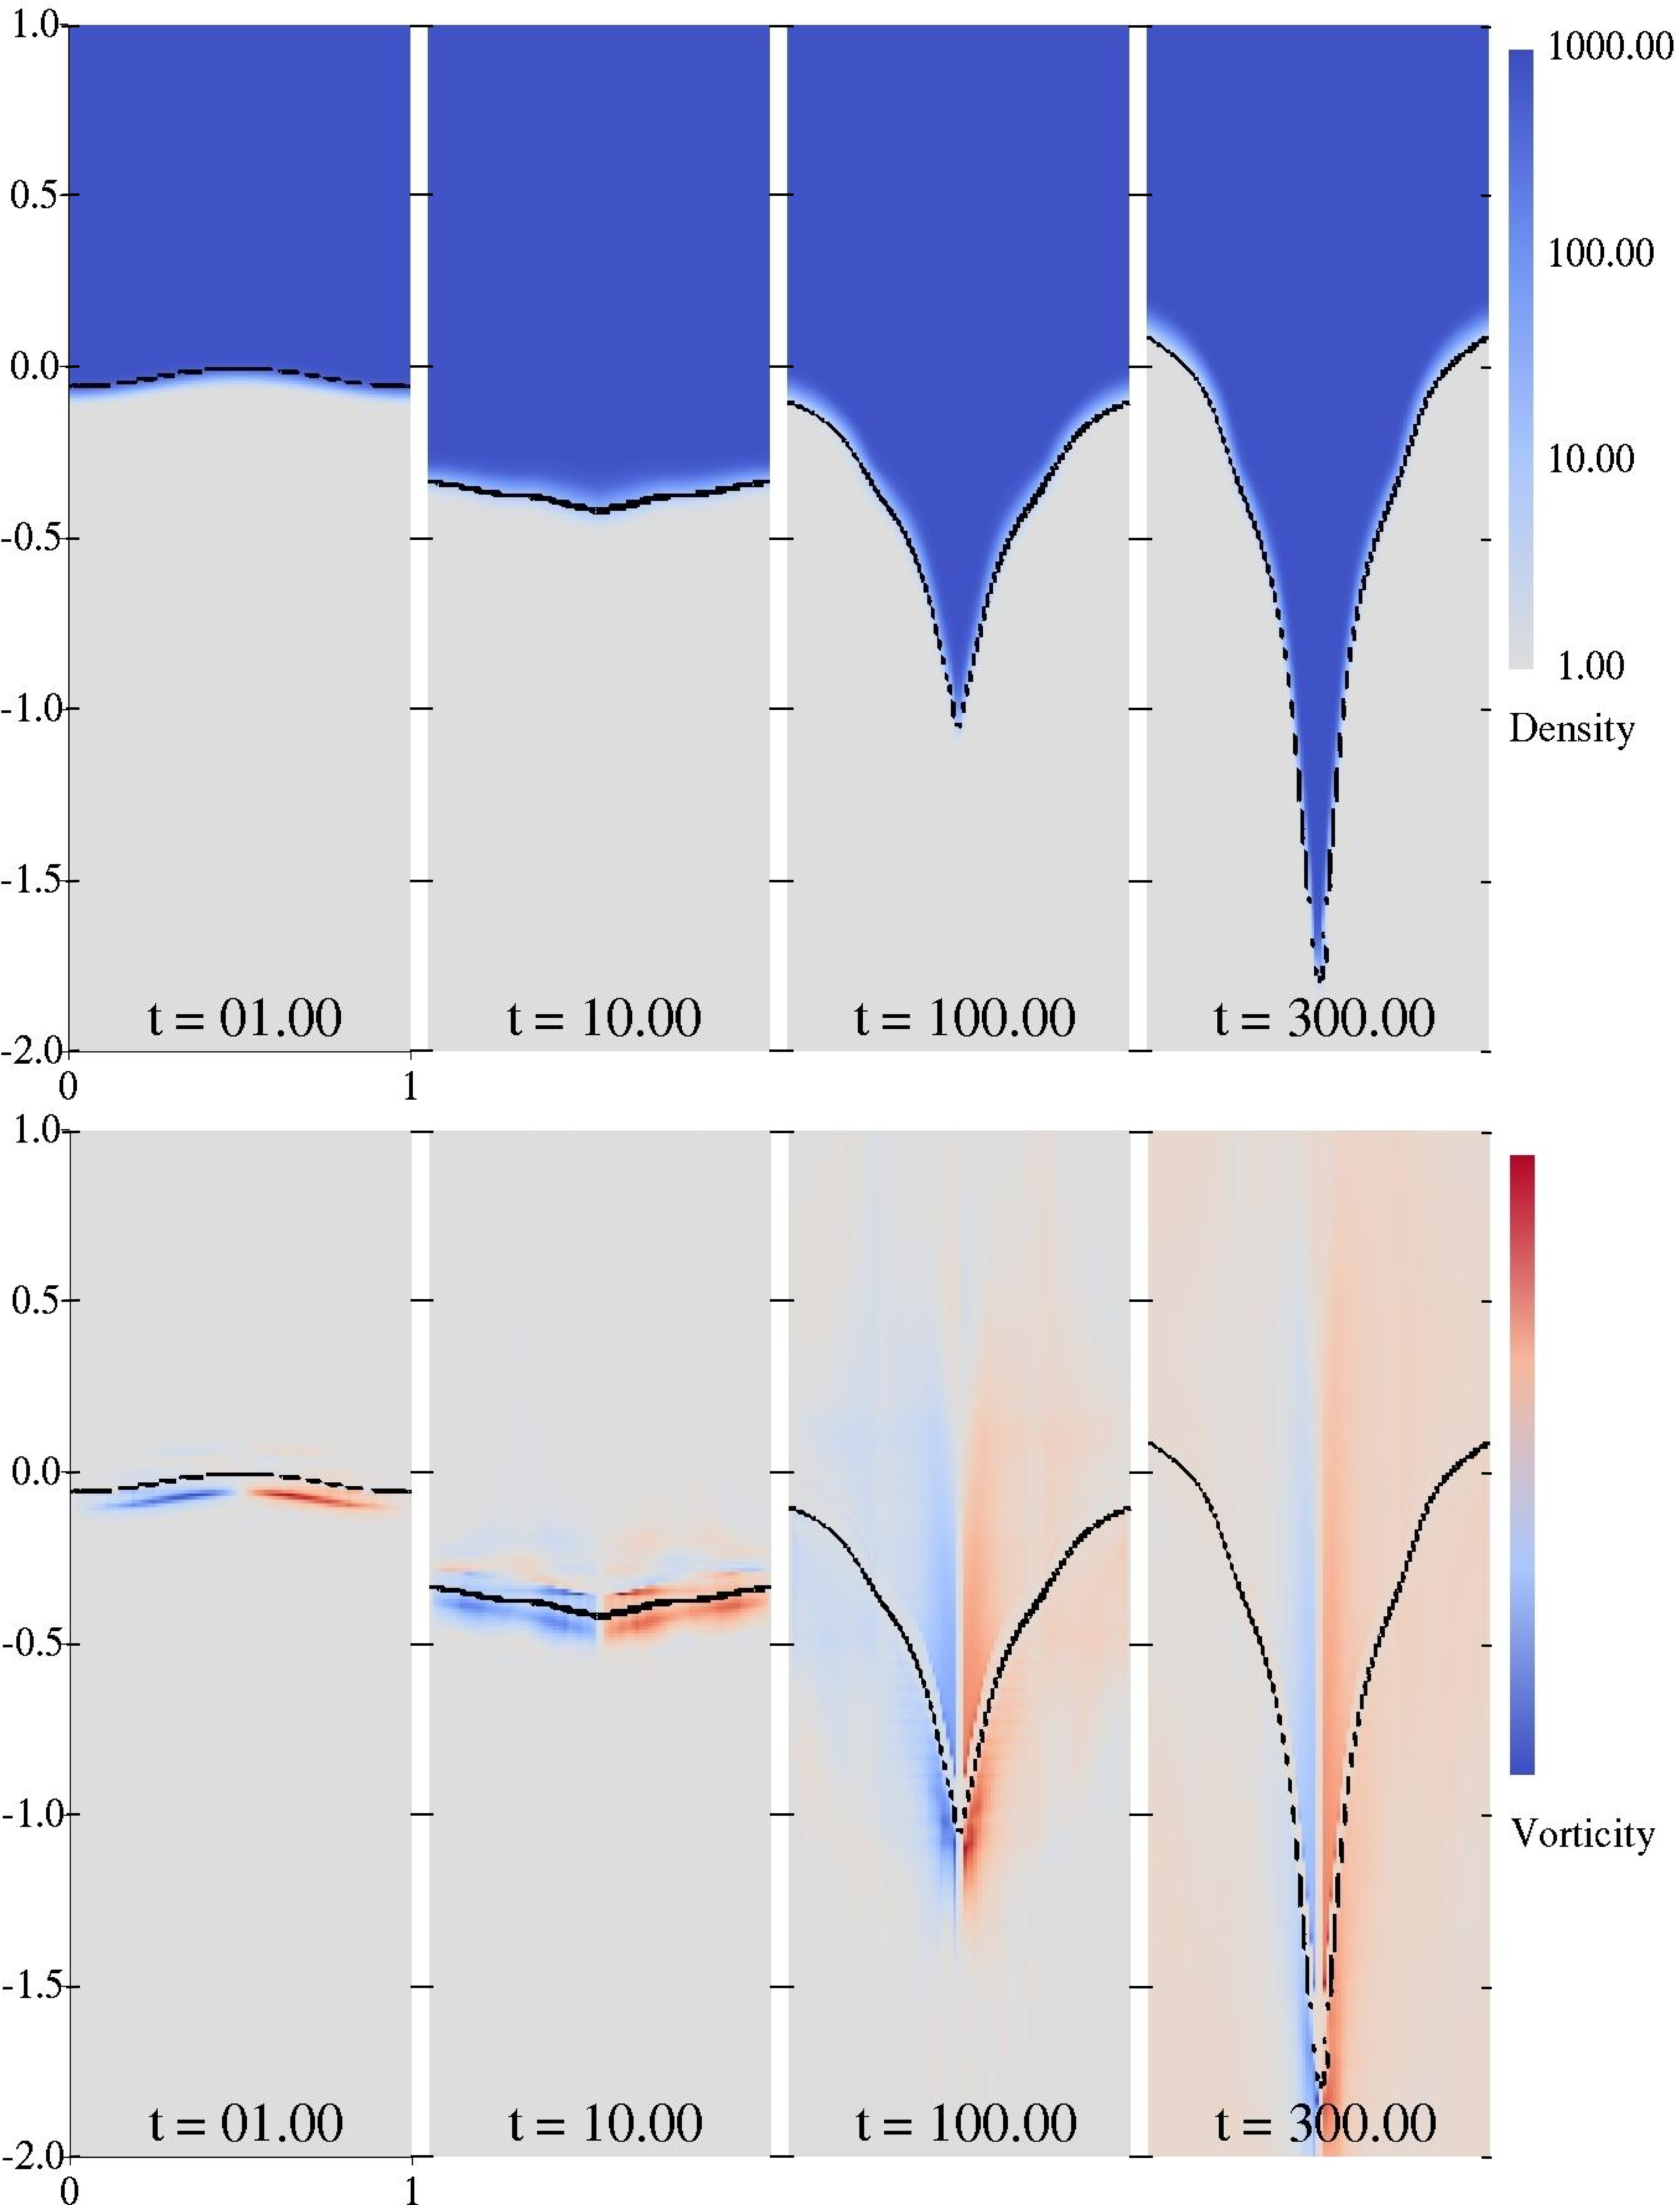
\includegraphics[width=0.9\textwidth]{./figs/lung_figs/snapshots_t1}
\caption[The evolution of the acoustically perturbed interface and vorticity field]{Surface plots of density (Top) and vorticity (Bottom)
  throughout the evolution of the interface for the $10$ MPa
  trapezoidal wave case. Areas of high density (i.e., water) are
indicated in dark blue. Areas of low density (i.e., air) are indicated
in white.  Positive (counterclockwise) vorticity is indicated in red,
and negative (clockwise) vorticity can be seen in blue.}
  \label{fig:interface_snapshots}
\end{figure}
%
\begin{figure}[h] 
  \centering
  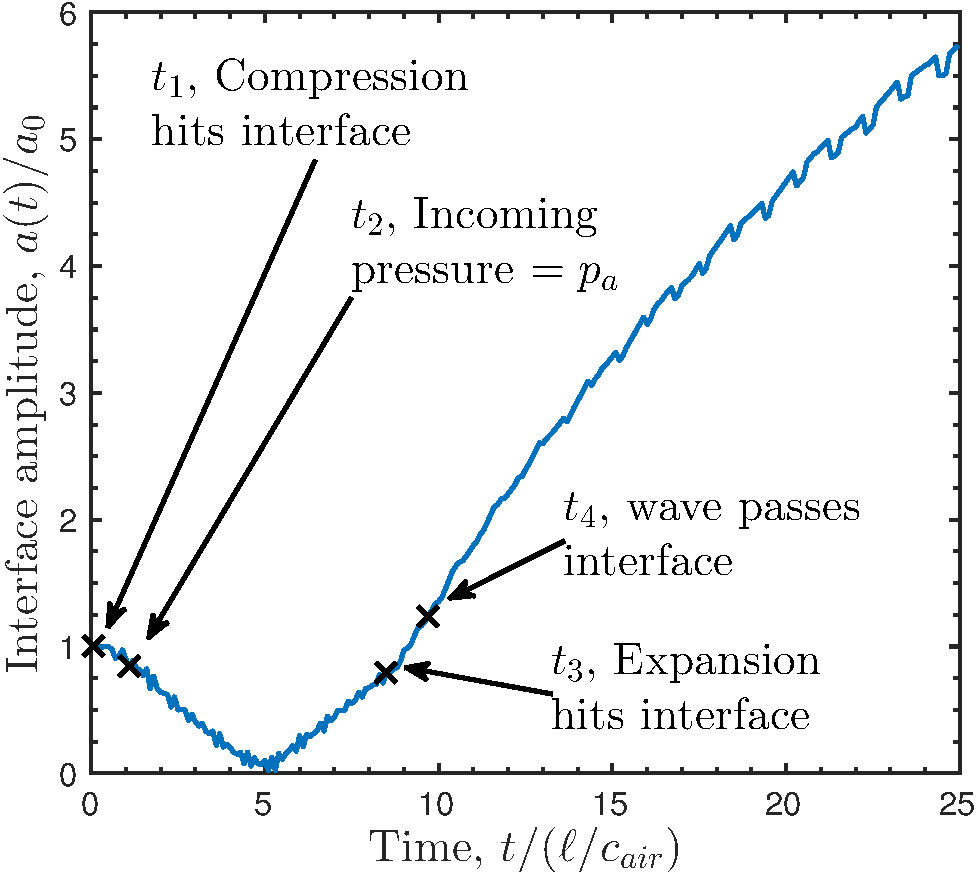
\includegraphics[width=0.48\textwidth]{./figs/lung_figs/trapz10_intf_schematic}
  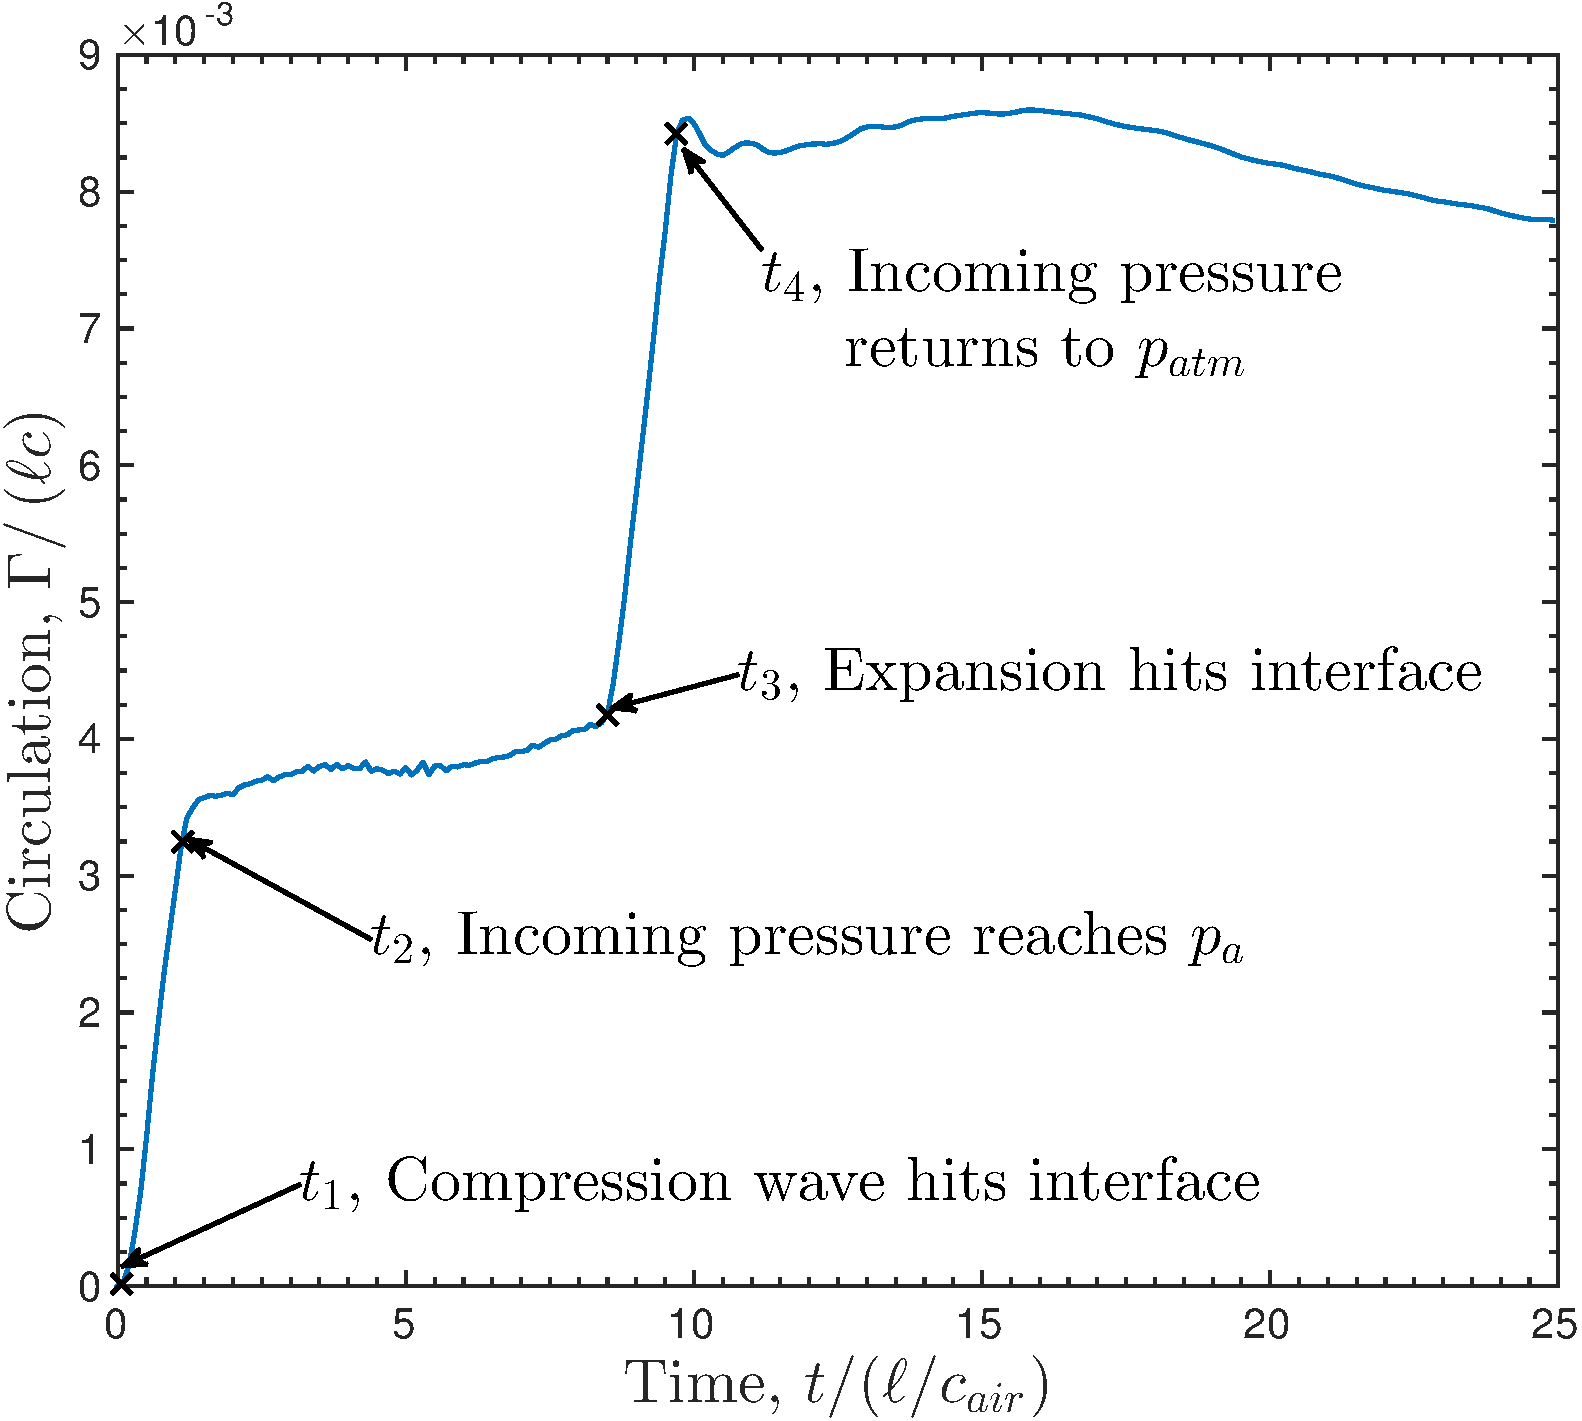
\includegraphics[width=0.48\textwidth]{./figs/lung_figs/trapz10_circ_schematic}
  \caption[The interface amplitude and circulation histories for the $10$ MPa trapezoidal wave]{The interface amplitude (left) and circulation (right)
    histories corresponding to the $10$ MPa trapezoidal waves are
    shown for $t\leq25$. Indicated times, $t_{1-4}$, are the times at
    which different stages of the incoming trapezoidal pressure wave
    shown in Figure \ref{fig:p0} first encounter the interface.}
  \label{fig:trapz10_circ_interface}
\end{figure}
%
%
\subsubsection{Dependence on acoustic wave amplitude}%
\label{subsubsec:amplitude_dependence}%
To investigate the dependence of the dynamics on the trapezoidal wave
amplitude, we compare results for $p_a=1$, $5$, and $10$ MPa while
keeping the initial lengths of the wave $L$ and the rise and fall
$\Delta L_a$ constant such that $p_a$ scales linearly with the
acoustic pressure gradient. Figure
\ref{fig:trapz_circ_interface_early}, illustrates the interface
amplitude and $p_a$-normalized circulation histories for $t\leq25$,
during and shortly after the wave-interface interaction. Black
$\bs{\times}$s along the curves indicate $t_{1-4}$, described
previously in Subsection \label{subsec:Qualitative}. During the
interaction between the interface and the compression wave, the rate
at which the perturbation amplitude decreases is greater for higher
amplitude waves. The circulation deposited during this period scales
linearly with $p_a$ as is consistent with baroclinically-generated
circulation based on our analysis. For the $10$ MPa wave, the phase of
the interface inverts at, before the expansion hits, causing
circulation deposited by the expansion to have the same sign as that
deposited by the compression. For the $1$ and $5$ MPa waves interface
phase inversion occurs after the expansion and consequently deposits
circulation opposite that of the compression wave.

Figure \ref{fig:trapz_circ_interface_loglog} \hl{(update this figure)}
shows the interface amplitude and circulation histories for $5$ and
$10$ MPa trapezoidal wave cases for $0 \leq t\leq 1000$. The
perturbation amplitude history is plotted on logarithmically-scaled
axes. For both waves, the slope of the perturbation amplitude is
approximately $0.60$ long after the waves have left the
interface. This is slightly higher than the 0.5 slope predicted by
scaling law \eqref{eq:intf_circ_scaling}. The results for the $1$ MPa
trapezoidal wave were not included because interface evolved too
slowly to obtain useful data given the computational resources available.
%
\begin{figure}[h] 
  \centering
  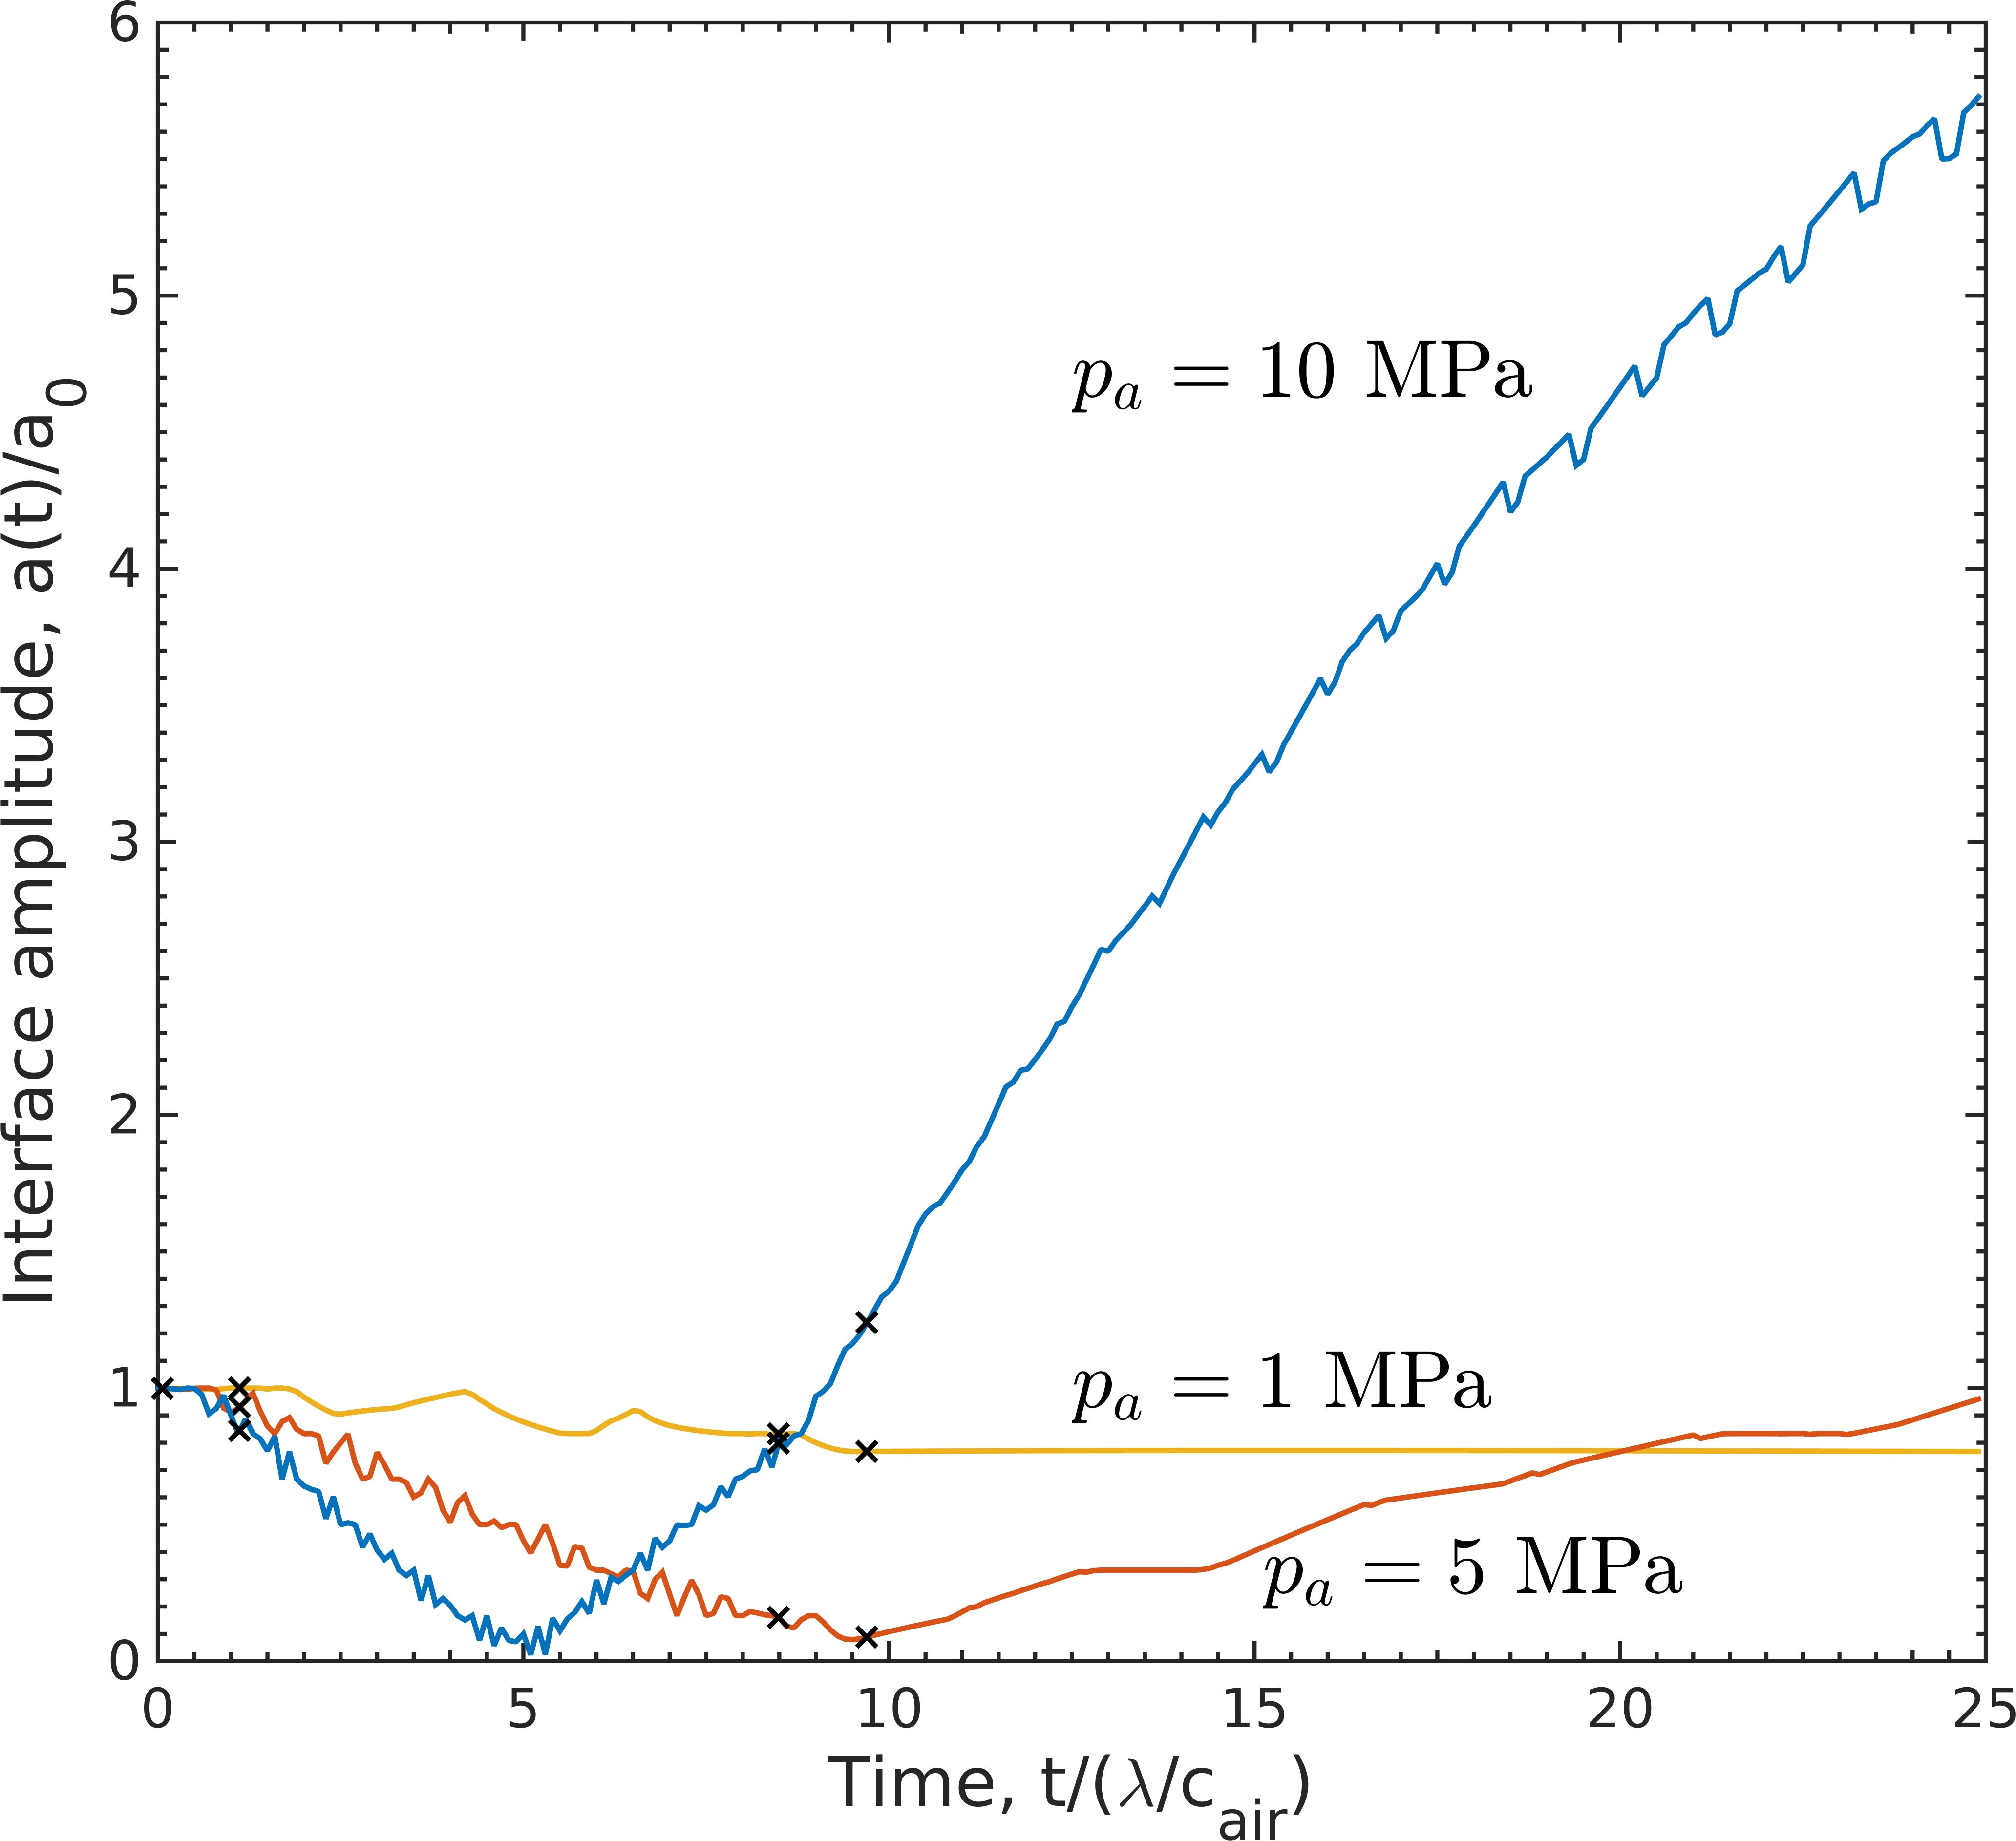
\includegraphics[width=0.48\textwidth]{./figs/lung_figs/interface_multi-amp_norm}
  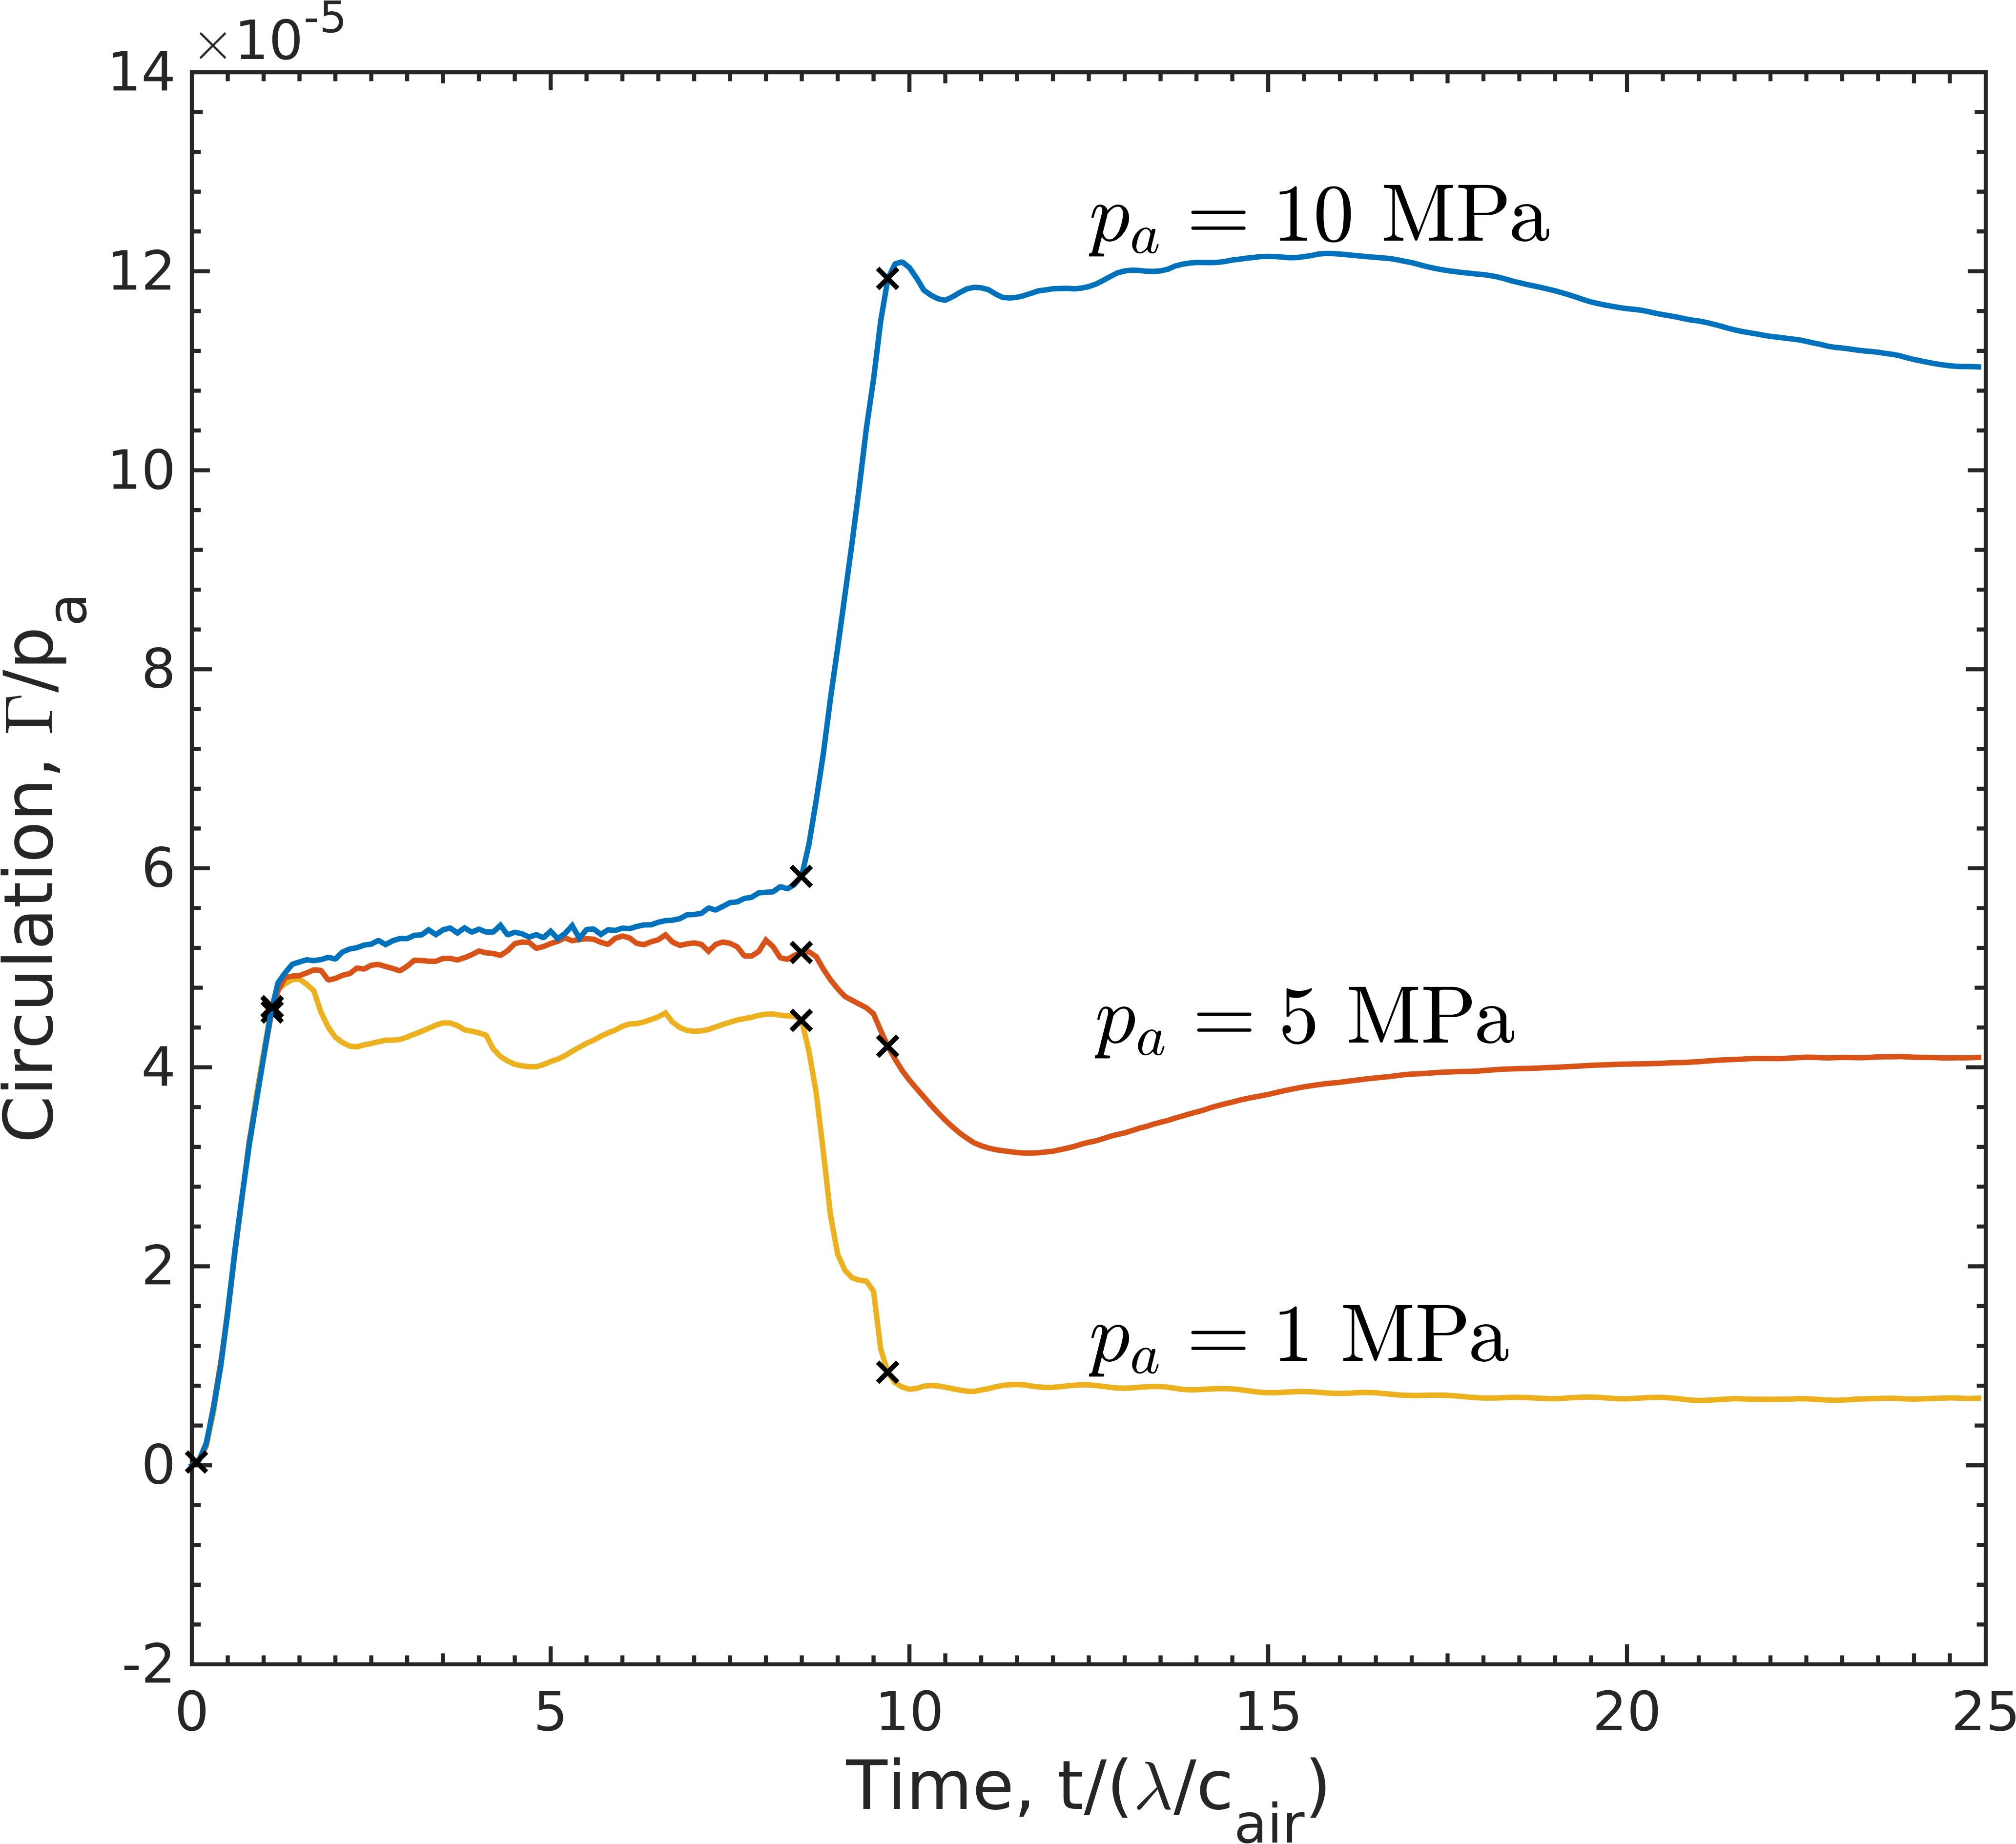
\includegraphics[width=0.48\textwidth]{./figs/lung_figs/circulation_multi-amp_norm}
  \caption[The interface and circulation dependence on wave amplitude at early time]{The interface amplitude (left) and circulation (right)
    histories corresponding to the $1$(yellow), $5$(orange), and
    $10$(blue) MPa trapezoidal waves are shown for $t\leq 25$. The
    circulation history is normalized by the acoustic amplitude of the
    incoming wave to illustrate that circulation deposition by the
    compression wave scales linearly with $p_a$.}
  \label{fig:trapz_circ_interface_early}
\end{figure}
%
\begin{figure}[h] 
  \centering
  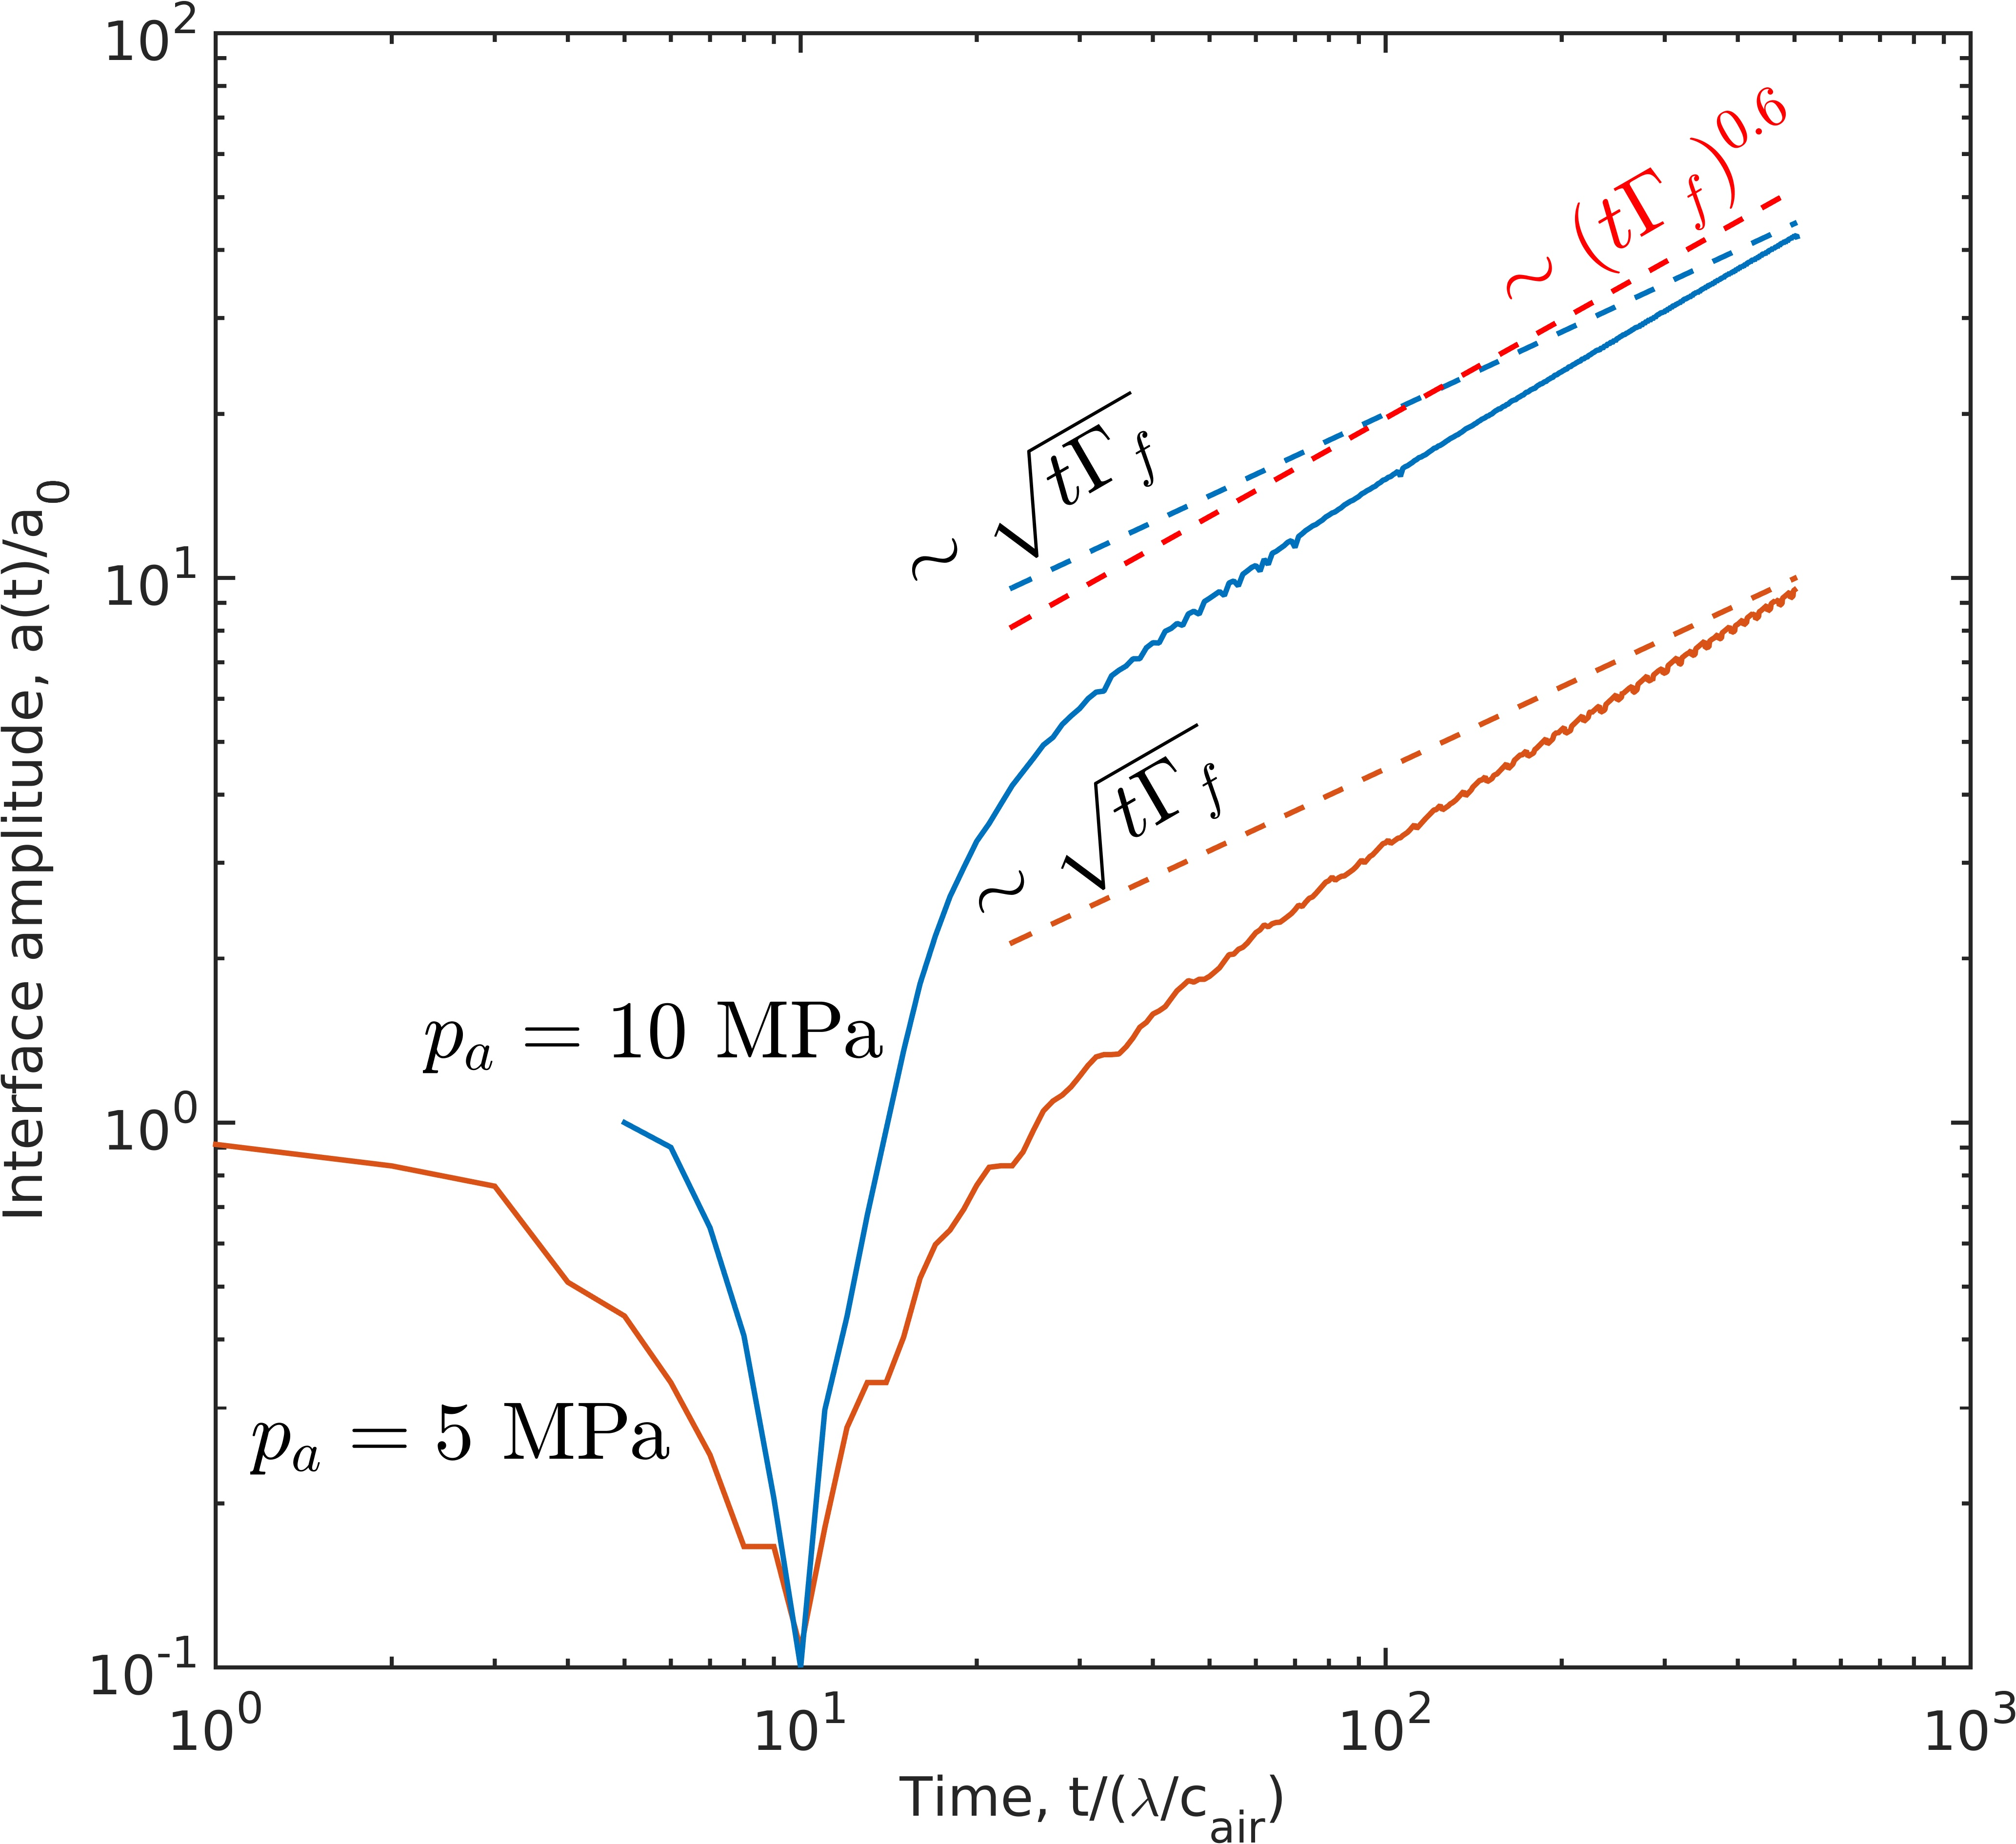
\includegraphics[width=0.48\textwidth]{./figs/lung_figs/interface_multi-amp_loglog_roe_extra}
  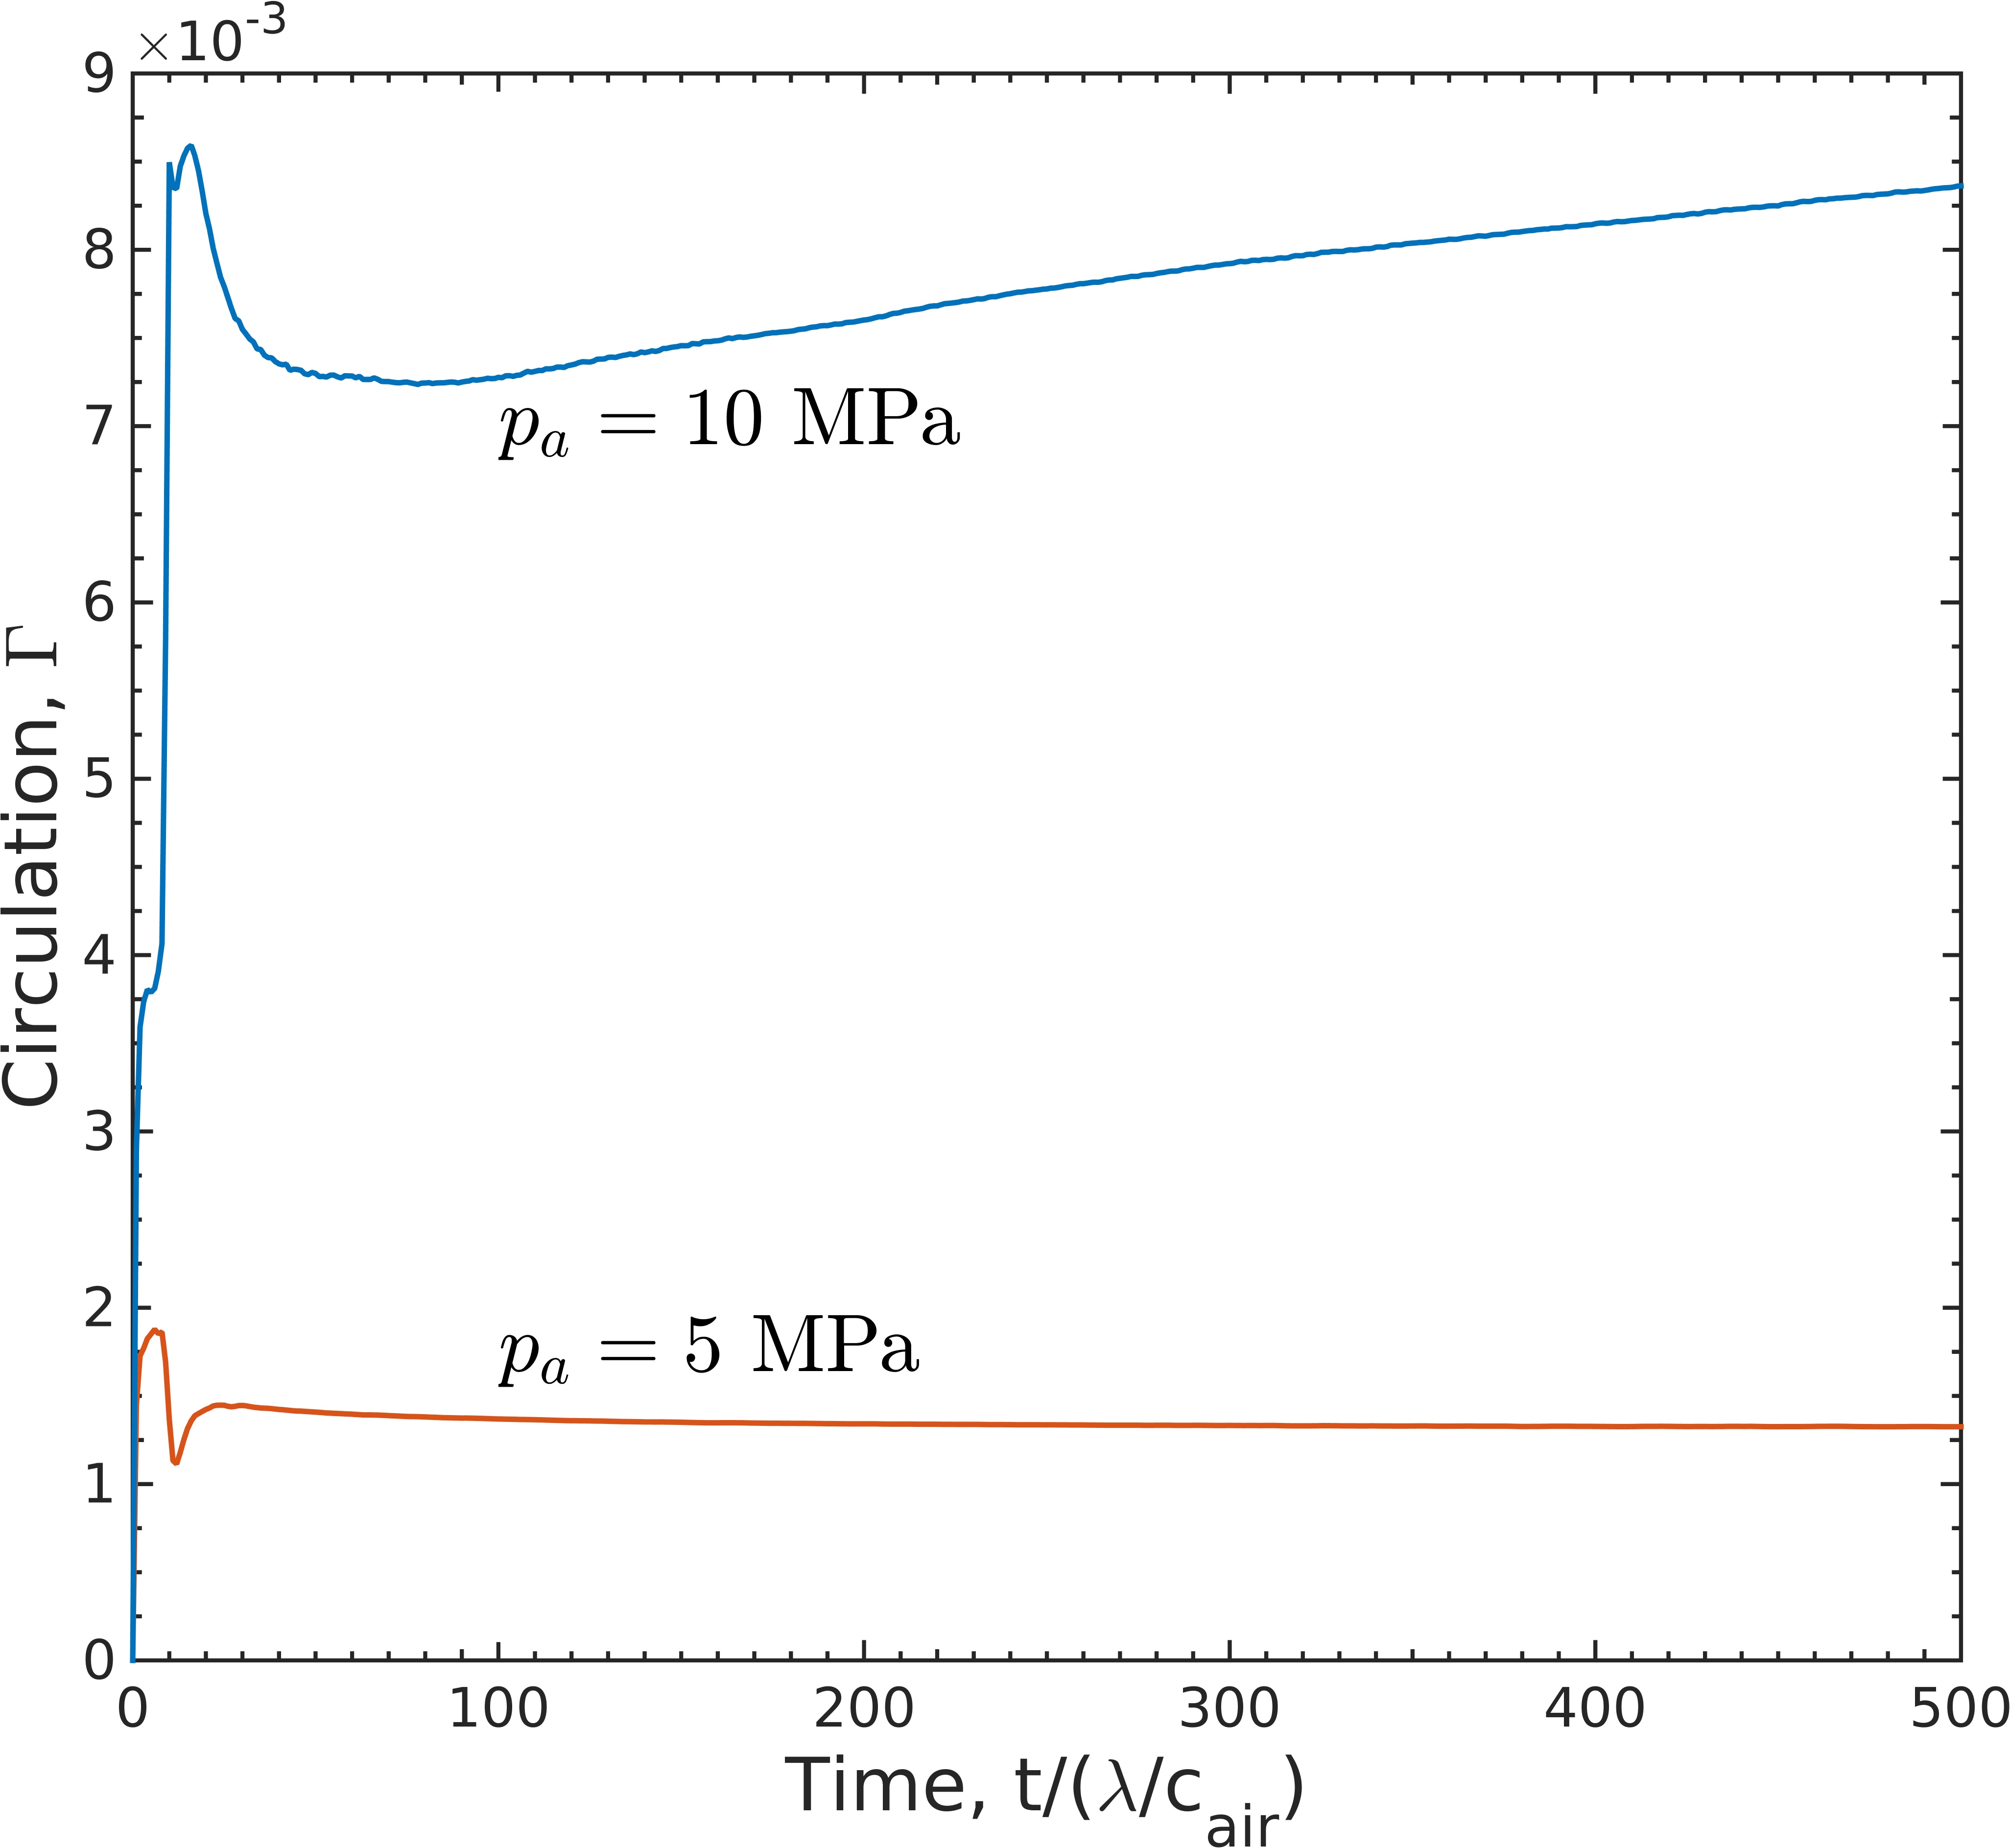
\includegraphics[width=0.48\textwidth]{./figs/lung_figs/circulation_multi-amp2_roe}
  \caption[The interface and circulation dependence on wave amplitude
  at long time]{The interface amplitude (left) and circulation (right)
    histories corresponding to the $5$(orange) and $10$(blue) MPa
    trapezoidal waves are shown for $t\leq 500$. To appropriately
    compare late time dynamics, time has been offset in the interface
    amplitude history such that the phase reversal appears to occur
    simultaneously in both simulations. Dashed lines of the same color
    are used to demonstrate the expected slope of pure circulation
    driven interface growth, based on Equation
    \eqref{eq:intf_circ_scaling}. The red dashed line shows the slope we
    appear to be approaching for the $10$ MPa wave case for the end time.}
  \label{fig:trapz_circ_interface_loglog}
\end{figure}
%
\subsubsection{Dependence on the length of the wave}%
To investigate the dependence of the dynamics on the length of the
trapezoidal wave $L$, and comparably the wave-interface interaction
time, we compare results for $p_a=10$ MPa waves of constant rise and
fall length $\Delta L_a$. This effectively changes the time the
interface has to evolve while experiencing the constant elevated
pressure portion of the wave between the compression and expansion.
Figure \ref{fig:trapz_circ_interface_multi-lag} shows the interface
amplitude and circulation histories corresponding to waves with
$L=45\lambda, 35\lambda ,30\lambda ,25\lambda ,15\lambda ,10\lambda$
for $0 \leq t\leq 25$.  For the three longest waves, $L \geq 30\lambda$,
the expansion encounters the interface after the perturbation reverses
phase. In these cases, the expansion deposits additional positive
circulation along the right half of the interface. For the shorter
waves, $L \leq 25\lambda$, the expansion encounters the interface before
the perturbation reverses phase and the net half-domain circulation is
decreased. Comparing cases in which the interface inverts phase before
the expansion occurs the larger $a(t)$ is at the time, the more
circulation is generated. The same is true when comparing cases in
which the phase inversion occurs after the interface inverts phase.
%
\begin{figure}[h] 
  \centering
  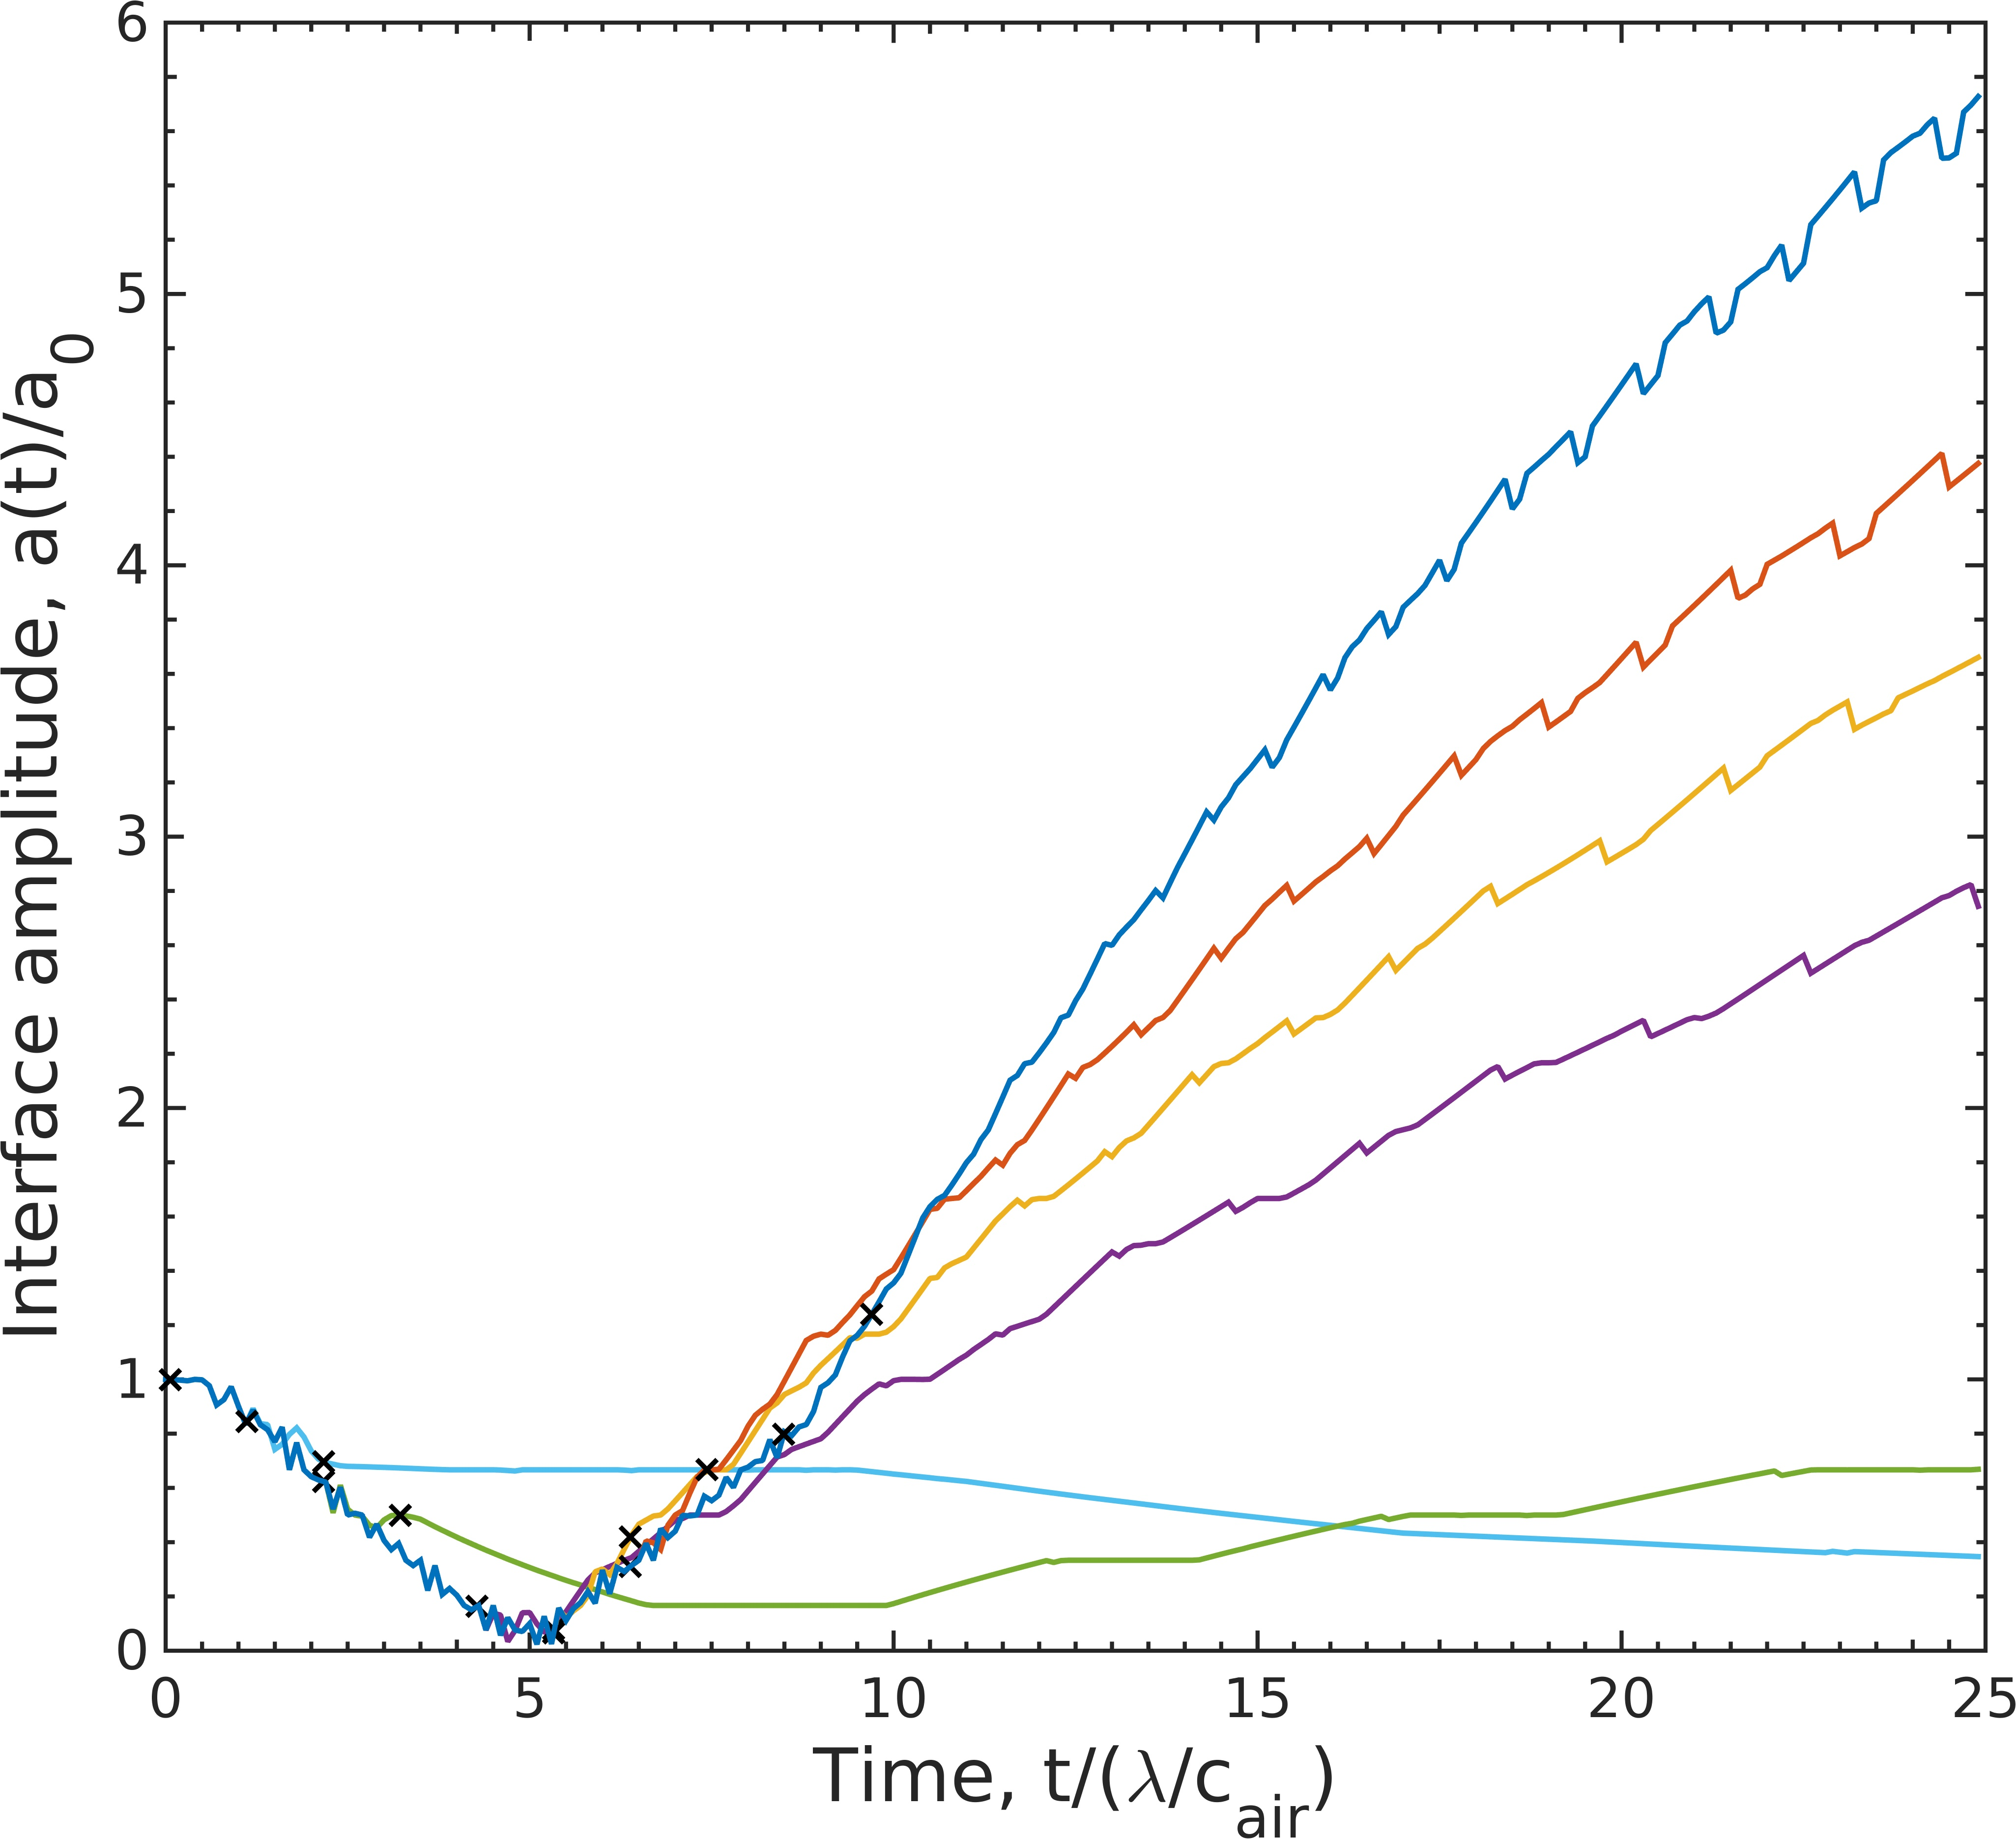
\includegraphics[width=0.48\textwidth]{./figs/lung_figs/interface_multi-lag}
  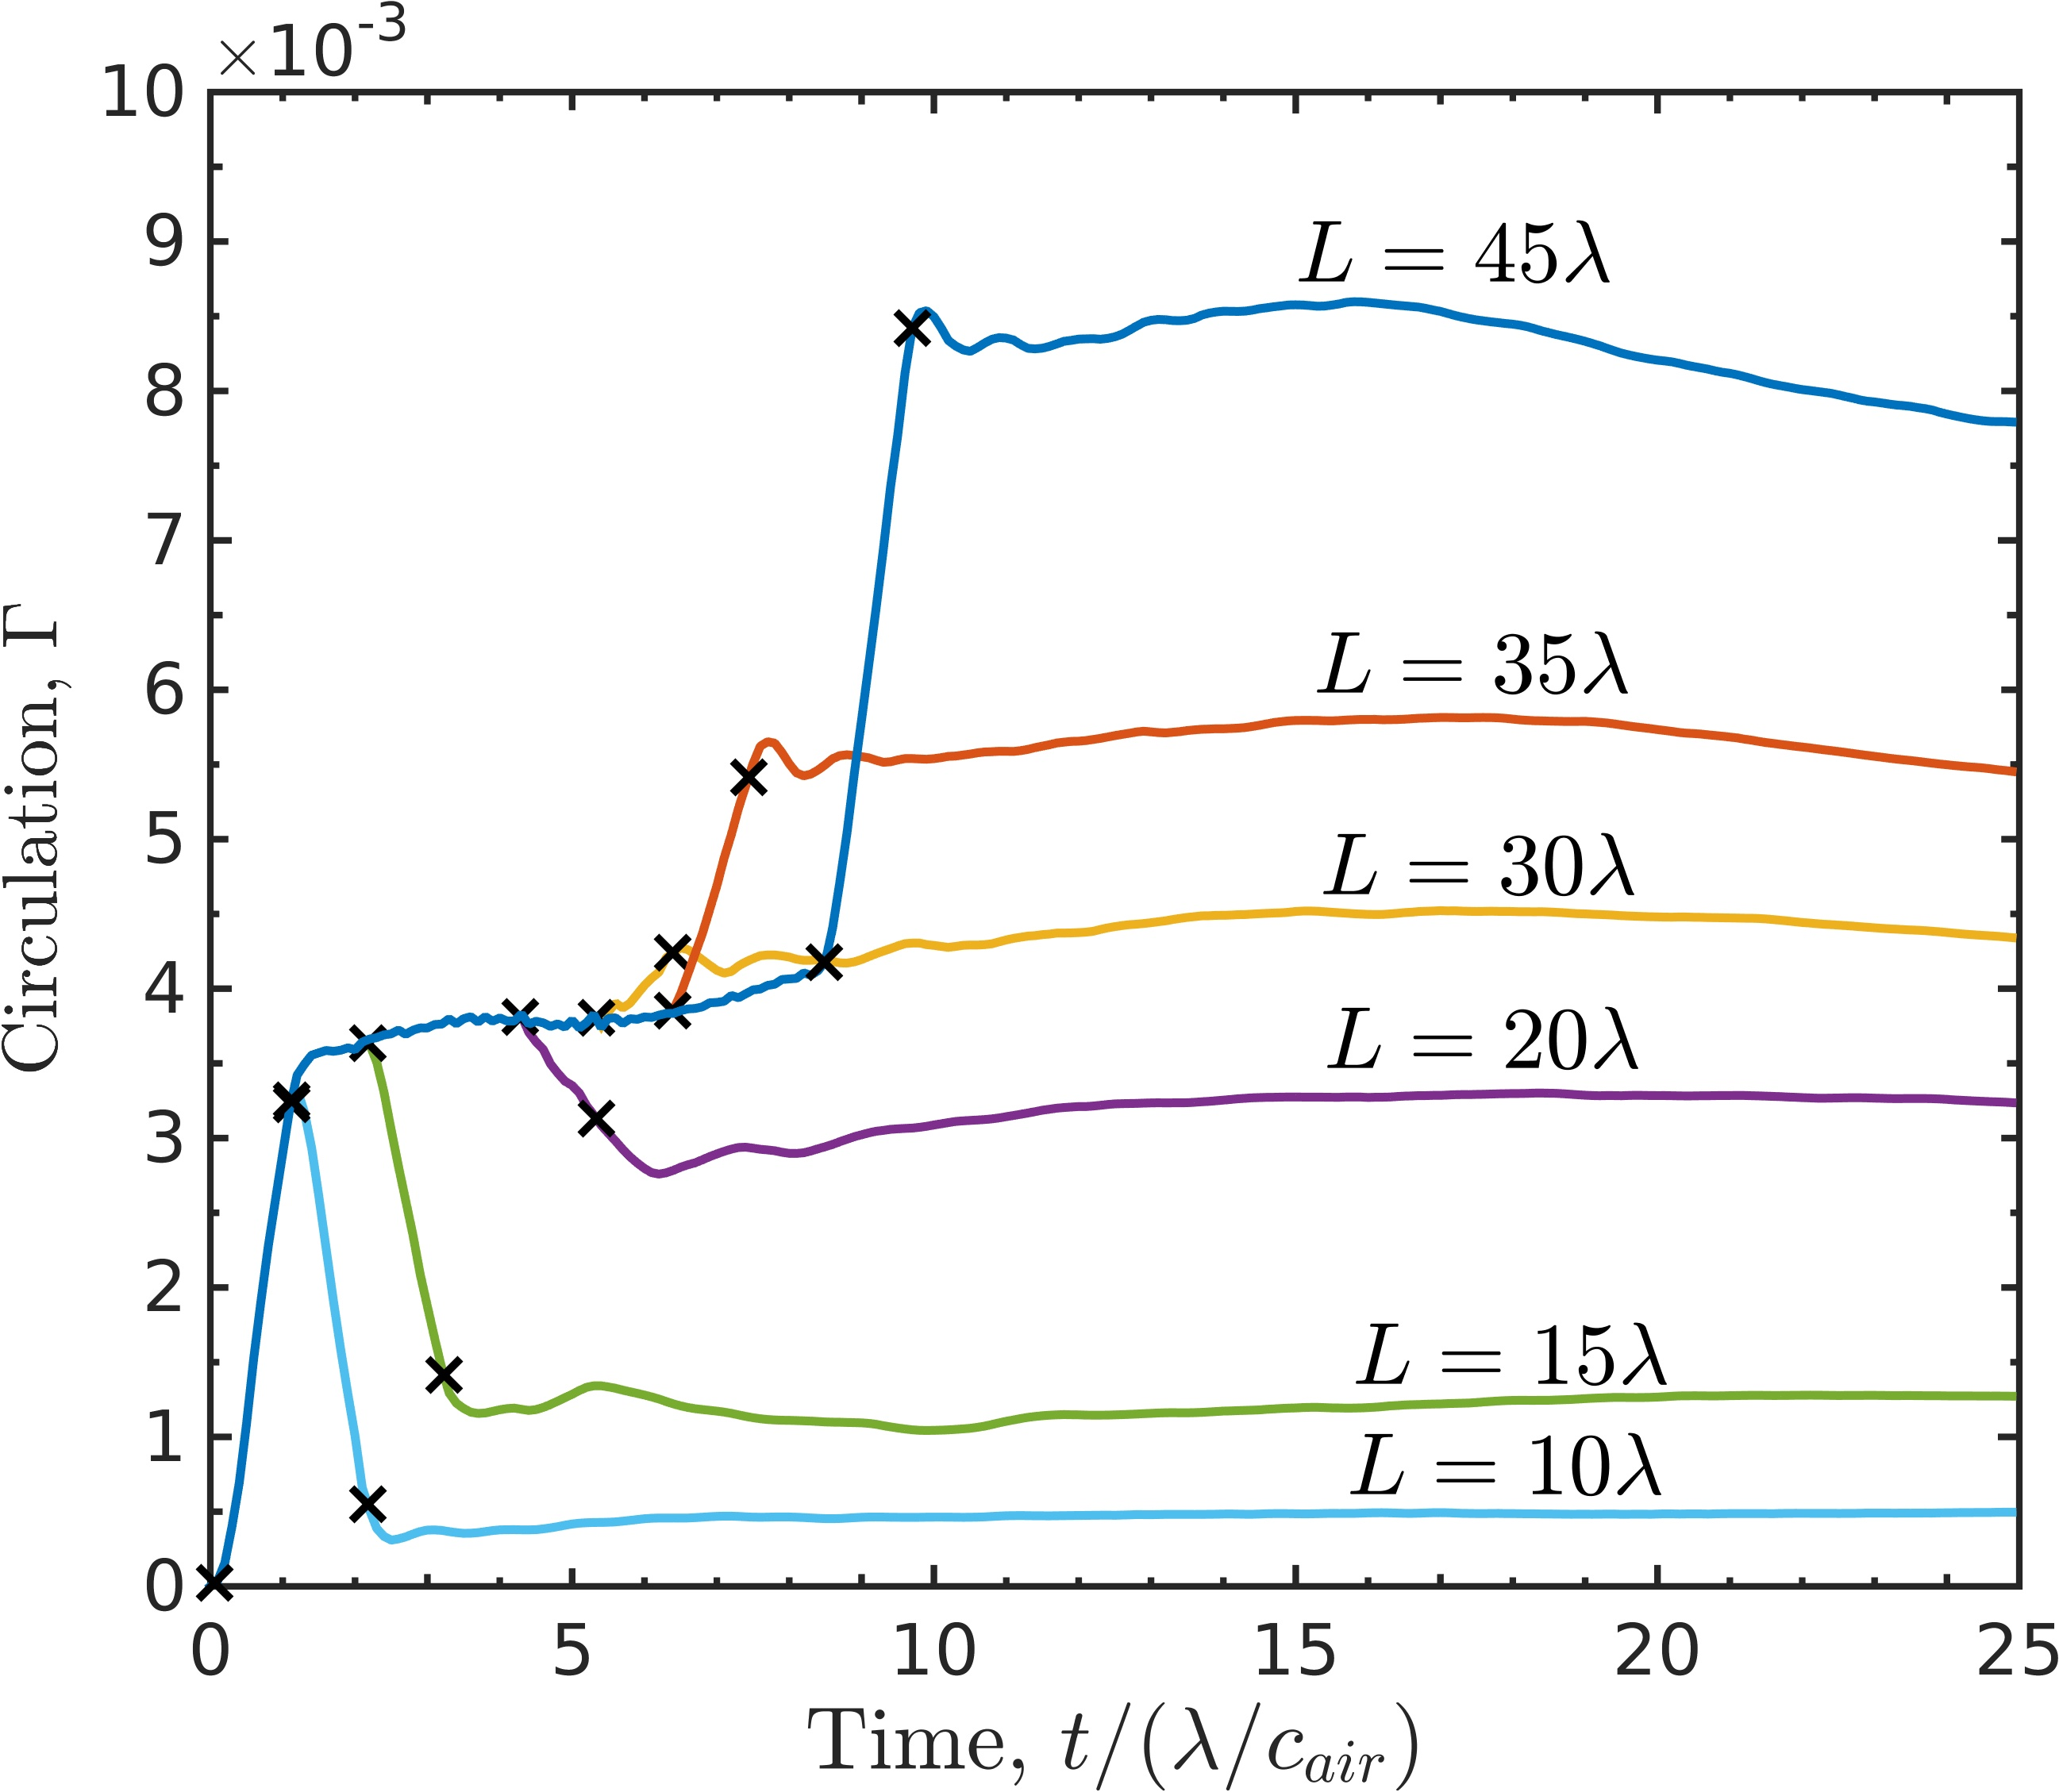
\includegraphics[width=0.48\textwidth]{./figs/lung_figs/circulation_multi-lag_fixed}
  \caption[The interface and circulation dependence on wave
  duration]{The interface amplitude (left) and circulation (right)
    histories for waves of varying total length $L$ and elevated
    static pressure duration between the expansion and compression
    . Here we show results for $L=45\lambda$ (blue), $L=35\lambda$
    (orange), $L=30\lambda$ (yellow), $L=20\lambda$ (purple),
    $L=15\lambda$ (green), $L=10\lambda$ (light blue)}
  \label{fig:trapz_circ_interface_multi-lag}
\end{figure}
%
\subsection{Discussion}
\label{subsec:discussion}
After the passage of the trapezoidal acoustic waves the pressure
returns to the initial, ambient conditions. This implies that the
integral of the pressure gradient $\nabla p$ along the interface, over
all time is zero. Hence we surmise that if the interface remains
unchanged during the interaction with the wave, as it would for a wave
moving with infinite velocity, $\nabla \rho$ would remain constant and
the net baroclinic circulation deposited must be zero. Thus for any
finite duration acoustic wave to deposit net baroclinic circulation
upon an interface, the interface itself must deform during interaction
with the wave. This deformation alters the misalignment of the
pressure and density gradients throughout the passage of the wave such
that vorticity deposited by the compression and expansion waves do not
cancel. Note that this of particular interest for waves in which
the pressure returns to the initial condition after the wave passes,
which is not the case for the traditional shock-accelerated \ac{RMI}
problem.

For the cases varying the length of the wave $L$, we previously noted
that whether the expansion increased or decreased the total
half-domain circulation depended on whether it encountered the
interface before or after the phase change. If indeed circulation is
driving the deformation of the interface, then changes in the waveform
that appear to have very little effect on the interface dynamics
during the wave-interface interaction period, may have far more
significant impacts on the long term dynamics of the interface via
vorticity.
%% Local Variables:
%%% mode: latex
%%% TeX-master: "../main"
%%% End:

\section{Summary and Conclusions}
\label{sec:conclusions}
This paper demonstrates that acoustic waves may trigger significant
deformation of perturbed liquid-gas interfaces over long periods of
time. The driving mechanism behind this deformation is baroclinic
vorticity, which occurs as a result of misalignment between the
pressure gradient of the acoustic wave and density gradient of the
perturbed interface. To demonstrate this we simulate trapezoidal
acoustic waves of MPa-order amplitude impinging from water onto
air.

The work presented here supports the following three conclusions: (1)
Acoustically-generated baroclinic vorticity is capable of
significantly deforming perturbed liquid-gas interfaces. We observed
that much of the vorticity generated by the acoustic wave at the
interface remains with the interface as it evolves and deforms even
long after the passage of all acoustic waves. Part of this is
attributed to a lack of physical mechanism for dissipating vorticity
in the inviscid case considered. From dimensional analysis we find
scaling law \eqref{eq:intf_circ_scaling}, suggesting that the
interface perturbation amplitude will grow as $t^{0.5}$ for purely
circulation driven growth. In our computed results we find the actual
perturbation amplitude grows as $t^{0.6}$. This slight discrepancy
could be a result of the inability of a global quantity $\Gamma$ to
completely describe $a(t)$ which is governed by local fluid mechanics.
%
(2) Baroclinic vorticity is predominantly deposited in the gaseous
fluid. We perform analysis to predict that on either side of an
infinitely sharp water-air interface, the vorticity generation rate
would be approximately two orders of magnitude greater on the air side
of the interface than in the water. This is qualitatively supported by
our computational results which find that near the end of the initial
compression wave-interface interaction nearly all of the circulation
exists in fluid dominated by air. For the $10$ MPa wave, for instance,
97\% of the circulation is found in fluid with volume fraction of
water $\alpha<0.5$ at $t=1$, after 91\% of the compression has passed.
%
(3) Changes in the acoustic waveform that have little effect on the
interface dynamics during their interaction can substantially effect
the interface over longer periods of time, via vorticity. By comparing
the effects of $10$ MPa trapezoidal waves with varying static pressure
durations between compression and expansion, we observe that the
evolution of the interface between these two wave components
drastically effects the ultimate growth rate of the interface. The
phase and amplitude of the interface perturbation at the time it
encounters the expansion wave determine the direction and magnitude
respectively of the vorticity deposited. Consequently, the amount of
vorticity remaining at the interface and in the surrounding fluid
after the passage of the wave changes greatly based on the
time-dependent features of the wave.

This work is a step toward understanding the effects of acoustically
generated vorticity on gas-liquid interfaces, but there are many
questions left to be answered. Physical effects not considered here
such as viscosity, which is critical to understanding the dissipation
of viscosity, may be highly important in certain
regimes. Additionally, to fully understand the application of these
findings to the motivating problem of diagnostic induced lung
hemorrhage, it will be important to consider waveforms and geometries
more relevant to the problem.


% \subsection{old}

% As such, we expect the late-time deformation to depend on the
% circulation in a predictable way. From dimensional analysis, we expect
% that the perturbation amplitude of a purely circulation driven
% interface will grow as $(\Gamma t)^{0.5}$ after all waves have
% passed. This is in contrast to our experimental results which find the
% amplitude to grow as $(\Gamma t)^{0.6}$. This discrepancy may be a
% result of the limitations of attempting to use circulation, a global
% quantity, to describe the perturbation amplitude, which depends on the
% local dynamics of the peaks and troughs of the interface.

% The actual deposition of circulation we expect to depend on the
% interface and acoustic waveform. We demonstrate analytically that the
% dominant form of vorticity is baroclinic, which is supported by the
% directly proportional increase in circulation deposited and acoustic
% pressure gradient for a linear increase in pressure impinging upon the
% interface. 




% Deformation of the interface that occurs during the interaction with
% the wave plays an important role in the total circulation deposited
% and hence in the deformation.

% For a linearly
% increasing pressure occurring over sufficiently short time that the
% interface does not deform appreciably, the amount of vorticity
% deposited scales linearly with the amplitude of pressure gradient.



% This work is unique in that we propose a previously unconsidered
% potential damage mechanism for \ac{DUS}-induced \ac{LH}. We
% hypothesize that baroclinic torque occurs at fragile air-tissue
% interfaces of the lung due to misalignment between the \ac{US}
% pressure gradient and material interface density gradient, causing
% stress, deformation, and ultimately rupture at the interface. This
% mechanism arises as a result of nonlinear, compressible fluid
% mechanics, and cannot be predicted through traditional linear
% acoustics. We suggest that nonlinear effects such as baroclinic
% vorticity are important to this problem because of the sharp density
% discontinuities between air and tissue within the lungs. To
% investigate our hypothesis we develop a numerical model of \ac{DUS}
% wave-alveolus interaction and simulate the physics underlying
% acoustically driven, perturbed liquid-gas interfaces.

% We aim to investigate three specific questions presented in Section
% \ref{sec:introduction}. To address these questions, we
% enumerate three conclusions of this work based on our results.  First,
% acoustic waves can generate vorticity at perturbed liquid-gas
% interfaces as a result of baroclinic torque. Second, this vorticity is
% capable of appreciably deforming the interface in the inviscid,
% inelastic case. We note that at this preliminary stage, additional
% simulations, run for longer time, will be useful in solidifying this
% conclusion.  Third, acoustic properties relevant to \ac{DUS} including
% acoustic amplitude, wave duration, and repetition frequency, are
% important to circulation deposition and subsequently any
% circulated-driven deformation or hemorrhage. For the case of a simple
% trapezoidal pressure wave, we demonstrate that the amount of
% circulation deposited along the interface scales linearly with the
% acoustic pressure amplitude. More subtly, because the interface is
% deforming throughout its interaction with the wave, affecting the
% alignment of pressure and density gradients, the acoustic wave
% duration can play an important role in determining how much
% circulation is ultimately deposited. Because the deformation can
% continue long after the wave has gone, similar arguments can be made
% for timing between subsequent waves. With regard to ultrasound, this
% could play an important role in choosing optimal \acs{PD} and
% \acs{PRF}.

%%% Local Variables:
%%% mode: latex
%%% TeX-master: "../main"
%%% End:










%\section{Future Work} \label{sec:usbe_lung_future}%
Finally, we address some of the limitations of this study and propose
future work to address some of these issues. To further evaluate the
relevance of the proposed damage mechanisms and presented results to
\ac{DUS}-induced lung hemorrhage, viscous and elastic effects should
be considered, as both of these have the potential to reduce observed
deformation, and mitigate hemorrhage. Additionally, more realistic
geometries that more accurately represent physical networks of alveoli
within the lungs will be useful to understand the propagation of
ultrasound waves and hemorrhage deeper into the lungs, beyond the
first tissue, air interface. To do this accurately, it may be
necessary to include a model for interface rupture. Many of these
future tasks will require not only additional numerical efforts, but
also experimental studies to appropriately characterize the lung
tissue and validate the suggested models. Additionally, to increase
our understanding of the relevant fluid dynamics, it will be important
it would be useful to be able predict the circulation and interface
dynamics based on the wave properties and initial conditions.

To address some of these issues and complete the proposed dissertation
research we plan to perform several tasks:

\begin{itemize}
\item To further the relevance of this research to the problem of
  \ac{DUS} of the lung we will:
  \begin{enumerate}
  \item Calculate stresses and strains at the interface compare to
    known properties of the lung. A passive viscous stress tensor will
    be computed from the velocity field and volume fraction fields,
    assuming constant viscosity for pure water and air. Lagrange
    particles will be placed upon the interface and tracked in time to
    calculate the pathlength of the interface as a function of time
    $S_{Intf}(t)$. This will be used to compute the engineering strain,
    $\varepsilon$, as though the interface were a solid sheet of
    tissue where, where
    $\varepsilon=[S_{Intf}(t=0)-S_{Intf}(t)]/S_{Intf}(t=0)$.
    % 
  \item Investigate the effects of alveolar side wall structures. To
    model this, a thin layer of tissue (modeled as water) will be
    placed at the edges of the alveolus (modeled as air) and periodic
    boundary conditions will be used.
    %
  \item Investigate the propagation of ultrasound waves and hemorrhage
    into the lungs. To model this we will modify the current geometry
    to such that a thin sinusoidal strip of water, parallel to the
    initial interface, will be be placed every $\lambda$ deep into the
    alveoli. This will be used with then be used with the alveolar
    walls described above to simulate a diagnostic ultrasound pulse
    propagating into a uniformly distributed alveolar network.
    %
  \end{enumerate}
  % 
\item To further our understanding of fluid mechanics
  associated with acoustically perturbed fluid interfaces we will:
  \begin{enumerate}
  \item Perform longer simulations to validate $a(t)\sim\sqrt{\Gamma t}$ scaling.
    % 
  \item Develop a model to predict the circulation deposited on a
    slightly perturbed interface by a simple compression or expansion
    wave. To do this, we will assume the interface is static during
    the interaction with the wave. Then, estimate the baroclinic term
    of the vorticity equation based on known interface and wave
    properties and linear acoustic relationships between state
    variables.
    %
  \item Develop a model to predict the interface phase-reversal time
    for a simple compression wave. This model will be based on the
    expected compression of the interface due to the rising pressure
    during the interaction with the wave, and the subsequent
    circulation driven deformation described by scaling law
    \eqref{eq:intf_circ_scaling}.
    %
  \item Design acoustic waveforms that utilize time dependent features
    and interface deformation to generate minimal circulation and
    interface growth. To do this, we will will aim to create waves
    that deposit vorticity of opposite sign and approximately equal
    magnitude before and after the interface phase change. One example
    of a wave that will be considered is a single period sinusoidal
    pressure wave that changes from the compression to expansion as
    the phase of the interface inverts.
    %
  \item Investigate the cause of late time circulation growth observed
    in some simulations. As can be seen from the circulation history
    for the $10$ MPa trapezoidal wave in Figure
    \ref{fig:trapz_circ_interface_loglog}, circulation continues to
    grow after all waves have left the domain. We plan to first
    determine if this effect is physical or numerical. If this effect
    is physical, we aim to determine the mechanism.
    %
  \item Investigate the dependence of circulation on the type of
    Riemann solver used. Though this document has not provided results
    to this effect, we have noticed that the amount of circulation
    produced by a given problem setup is roughly twice as large when
    the Rusanov solver is implemented as opposed to Roe solver. We
    will investigate the cause of this in order to determine which is
    more appropriate for our work.
  \end{enumerate}
\end{itemize}







% \begin{comment} Move this stuff to introduction There has been a
%   significant amount of prior research into ultrasound-induced
%   pulmonary hemorrhage, but in spite of this there are still many
%   questions left unanswered.  Presently the underlying damage
%   mechanism causing the hemorrhage is not currently known.  Research
%   has shown that the underlying mechanism of US-induced pulmonary
%   hemorrhage is non-thermal. \citet{Zachary2006a}, for instance,
%   compared lesions generated with DUS to those generated via laser
%   and found multiple differences in the injured tissue. Other
%   studies have shown that inertial cavitation, the intially
%   suspected mechanism, is also unlikely to be responsible for the
%   US-induced PH. \citet{Raeman1997} injected the UCA Albunex, which
%   is expected to nucleate cavitation when exposed to US, into mice
%   before performing pulmonarry US and showed that the hemorrhage was
%   similar to that observed in control mice injected with saline.  In
%   a later study \citet{Obrien2000} placed mice under increased
%   hydrostatic pressure, to suppress the occurence of inertial
%   cavitation, before exposure to pulmonarry US, and found that
%   hemorrohage was enhanced by the increased pressure. While it is
%   widely suspected that the cause of the hemorrhage is mechanical,
%   the precise underlying mechanism by which acoustic energy is
%   tranduced into mechanical stress and strain in the capillary has
%   remained elusive.

%   We hypothesize that sharp pressure gradients in the US wave
%   interact with the strong density gradients at the blood-air
%   barriers in the lungs, in turn generating baroclinic vorticity at
%   the interface between the alveoli and the adjacent capillary
%   sheets.  Furthermore, we propose that this vorticity drives the
%   growth of this interface, causing strain, stress, and ultimately
%   failure.
% \end{comment}


% The future work investigating ultrasound-induced pulmonarry
% hemorrhage will be divided into two tasks.  First, further numerical
% simulations of liquid-gas interfaces with pressure waves will be
% performed in order to investigate US-generated baroclinic vorticity
% in the lung as a possible mechanism for hemorrhage. Second a
% simplified model of ultrasound propagation into the lung will be
% created.

% \section{Numerical investigation of ultrasound-lung interaction}
% To investigate the behavior of tissue-air interfaces with DUS waves,
% the lung will be modeled as a compressible fluid system.  As in the
% prior work, the alveoli will be modeled as air. The surrounding
% tissue will be treated as a Newtonian fluid with the density and
% viscosity of blood and all other relevant properties will be set to
% those of water. The liquid-gas interface will be modeled as a
% sinusoid of wavelength $\lambda=200\mu$m, as is consistent with
% typical alvelolar diameter (ADD CITATION). A series of simulations
% will be performed in which this liquid-gas interface will be
% subjected to a pressure waveforms of increasing complexity.

% \section{Baroclinic vorticity generation at the alveolar-capillary sheet interface blood-air barrier}
% \subsection{Estimations of vorticity generation}
% \subsection{Expected interface growth from vorticity at the
% interface }

% \section{Simulations of acoustic wave interactions with a sinusoidal blood-air interface}
% \begin{itemize}
% \item Proposed experiment 1: Interaction of a sinusoidal blood-air interface with a planar acoustic wave with linearly-increasing amplitude
% \item Proposed experiment 2: Interaction of a sinusoidal blood-air interface with a sinudoidal pressure pulse
% \item Proposed experiment 3: Interaction of a sinusoidal blood-air interface with a single DUS pulse
% \item Proposed experiment 4: Interaction of a sinusoidal blood-air interface with multiple DUS pulses
% Space pulses based on accepted experimental procedure and see how the secondary pulses effect the interaface growth.
% \end{itemize}

% \section{Modeling US propagation into the lung}
% I aim to model the propagation of ultrasound waves into the lungs.  Much of the lung is composed of tiny air-filled sacs called alveoli. Due to the large impedance mismatch between these alveoli and their surrounding tissue, the lung is highy acoustically reflective.

% \subsection{Propogation of acoustic energy into the lung}
% Use linear acoustics to predict the transmitted and reflected acoustic pressure amplitudes for air pockets separated by thin water (blood) membranes.  (1a) Model adjacent alveoli as first as normal planar slabs of air with thickness equal to alveolar diameter ($200\mu$m), seperated by slabs of water (blood) of alveolar membrane diameter ($1\mu$m).  (1b) Then model packed regular triangles, (1c) squares (faces oriented at π/4 relative to incoming plane wave.


%%% Local Variables:
%%% mode: latex
%%% TeX-master: "../main"
%%% End:




% 
%% Using AIAA bibliography.
\bibliographystyle{./tex/myauthordate2}

% Give this command the relative path to the .bib file.
\bibliography{../../../literature/library}
%
% 
\end{document}

%%% Local Variables:
%%% mode: latex
%%% TeX-master: t
%%% End:
